\documentclass[twoside,english]{Dianab5portrait}
\usepackage{import}


\title{Budget Repair}
\author{John Daley \and Danielle Wood \and Brendan Coates}

\addbibresource{../bibliography.bib}
\addbibresource{Hot-property-CG-and-NG/bibliography2.bib}

\usepackage{booktabs}
\usepackage{amsmath}
\usepackage{siunitx} % for decimal points in tables
\sisetup{detect-all} % to ensure helvetica is used
\usepackage{longtable} % session info
\usepackage{tabularx}  % boxed tables
%\usepackage{flushend}  % for flushed columns at end of chapters % too dangerous!
%    \raggedend  %% turn off except when manual
\usepackage{makecell}
\usepackage{multirow}
\usepackage{subcaption}
\captionsetup[subfigure]{skip=0pt, position=top, list=no, justification=centering, labelsep=space, labelfont=bf, font={bf,small,theGrey}}
% to prevent legend moving
\usepackage[noadjust]{marginnote}
\usepackage{grfext}
\usepackage{ragged2e}
%\raggedright
\usepackage[normalem]{ulem}  % for uline
\PrependGraphicsExtensions*{.pdf}
\usepackage{enotez}
\usepackage{ocgx}
\usepackage{enumitem}
\usepackage{trace}

\DeclareInstance{enotez-list}{custom}{paragraph}{%
 heading = \addchap{Endnotes}\DEVIATION{#1},
 notes-sep = 5pt,
 format = \footnotesize 
}

\let\originalfootnote\footnote
\let\footnote\endnote
% for a footnote that must be a footnote (not an endnote)
\newcommand{\FOOTNOTE}[1]{\originalfootnote{#1}}
\renewcommand*{\thefootnote}{\textrm{\fnsymbol{footnote}}}


\providecommand{\stopifendnote}[1]{}

\newcommand{\TBD}[1]{\colorbox{yellow}{#1}}
\newcommand{\defi}[1]{\textbf{#1}}
\newcommand{\DEVIATION}[1]{}

\newcommand{\taxabbrevT}{T}
\newcommand{\taxabbrevt}{t}
\newcommand{\taxabbrevE}{E}
\newcommand{\TEE}{TEE}
\newcommand{\TTE}{{TTE}}
\newcommand{\EET}{{EET}}
\newcommand{\ETT}{{ETT}}
\newcommand{\ttE}{tt{E}}
\newcommand{\ttt}{ttt}
\newcommand{\TtE}{TtE}

%
% wrong kerning?
\newcommand{\ATO}{A\/TO}
%

% Allow figure captions to run into margins
\usepackage{ifoddpage}
\newlength\fullwidth\fullwidth=\textwidth \advance\fullwidth by \marginparwidth
\advance\fullwidth by \marginparsep

\newlength\extraWd
\setlength\extraWd{\dimexpr\marginparwidth+\marginparsep\relax}
%\captionsetup{margin={0cm,-\extraWd}}

% bold headers in tabularx
\newcommand{\tblHead}  [2][c]{\bfseries\begin{tabular}[#1]{@{}l@{}}#2\end{tabular}}
\newcommand{\tblHeadR} [2][c]{\bfseries\begin{tabular}[#1]{@{}>{\raggedleft}p{\linewidth}@{}}#2\end{tabular}}
\newcommand{\tblHeadRm}[2][c]{\bfseries\begin{tabular}[#1]{@{}>{\raggedleft}m{\linewidth}@{}}#2\end{tabular}}
\newcommand{\tblHeadRb}[2][c]{\bfseries\begin{tabular}[#1]{@{}>{\raggedleft}b{\linewidth}@{}}#2\end{tabular}}
\newcommand{\tblHeadRR}[2][c]{\bfseries\begin{tabular}[#1]{@{}>{\raggedleft}p{\linewidth}@{}}#2\end{tabular}}
\newcommand{\tblHeadL} [2][c]{\bfseries\begin{tabular}[#1]{@{}>{\raggedright}p{\linewidth}@{}}#2\end{tabular}}
% right-aligned for tables
\def\barr{\begingroup\renewcommand{\arraystretch}{1}\begin{tabular}[c]{>{\bfseries}r}}%
\def\earr{\end{tabular}\endgroup}
% left aligned for tables
\def\barl{\begingroup\begin{tabular}[c]{>{\bfseries}l}}%
\def\earl{\end{tabular}\endgroup}

\newcommand{\tblHeadVC}[1]{\bfseries\begin{tabular}[c]{@{}>{\raggedleft}m{\linewidth}@{}}#1\end{tabular}}
\newcommand{\tblHeadVCL}[1]{\bfseries\begin{tabular}[c]{@{}>{\raggedright}m{\linewidth}@{}}#1\end{tabular}}
\newcommand{\tblHeadBCL}[1]{\bfseries\begin{tabular}[b]{@{}>{\raggedright}b{\linewidth}@{}}#1\end{tabular}}

\newcommand{\tblHeadVCHL}[1]{\barr\textbf{#1}\earr}
\newcolumntype{R}{>{\raggedleft\arraybackslash}X}
\newcolumntype{C}{>{\centering\arraybackslash}X}
\newcolumntype{Y}{>{\raggedleft\arraybackslash}X}

\newlength\Origarrayrulewidth
\newlength\Origbelowrulesep
\newlength\Origaboverulesep

% horizontal rule equivalent to \cline but with 2pt width
% for super acccumulation benefits table
\newcommand{\ClineDarkOrange}[1]{%
 \noalign{\global\setlength\Origarrayrulewidth{\arrayrulewidth}}%
 \noalign{\global\setlength\Origbelowrulesep{\belowrulesep}}%
 \noalign{\global\setlength\Origaboverulesep{\aboverulesep}}%
 \noalign{\global\setlength\belowrulesep{0pt}}%
 \noalign{\global\setlength\aboverulesep{0pt}}%
 \noalign{\global\setlength\arrayrulewidth{0pt}}\arrayrulecolor{DarkOrange}\cmidrule[1pt](l{-1pt}){#1}%
 \noalign{\global\setlength\arrayrulewidth{\Origarrayrulewidth}}%
 \noalign{\global\setlength\belowrulesep{\Origbelowrulesep}}%
 \noalign{\global\setlength\aboverulesep{\Origaboverulesep}}%
}

\newcommand{\ClineOrange}[1]{%
 \noalign{\global\setlength\Origarrayrulewidth{\arrayrulewidth}}%
 \noalign{\global\setlength\Origbelowrulesep{\belowrulesep}}%
 \noalign{\global\setlength\Origaboverulesep{\aboverulesep}}%
 \noalign{\global\setlength\belowrulesep{0pt}}%
 \noalign{\global\setlength\aboverulesep{-1pt}}%
 \noalign{\global\setlength\arrayrulewidth{0pt}}\arrayrulecolor{Orange}\cmidrule[1pt](l{-1pt}){#1}%
 \noalign{\global\setlength\arrayrulewidth{\Origarrayrulewidth}}%
 \noalign{\global\setlength\belowrulesep{\Origbelowrulesep}}%
 \noalign{\global\setlength\aboverulesep{\Origaboverulesep}}%
}


\newcommand{\boxsource}[1]{\vfill\footnotesize\textit{Source: }#1}
\newcommand{\boxsources}[1]{\vfill\footnotesize\textit{Sources: }#1}

\usepackage{environ}
\makeatletter
\newsavebox{\measure@tikzpicture}
\NewEnviron{scaletikzpicturetowidth}[1]{%
  \def\tikz@width{#1}%
  \def\tikzscale{1}\begin{lrbox}{\measure@tikzpicture}%
  \BODY
  \end{lrbox}%
  \pgfmathparse{#1/\wd\measure@tikzpicture}%
  \edef\tikzscale{\pgfmathresult}%
  \BODY
}
\makeatother

%  http://tex.stackexchange.com/questions/120716/appendix-after-each-chapter
\usepackage[page, toc]{appendix}
\usepackage{chngcntr}

\makeatletter
\@addtoreset{chapter}{part}
\@addtoreset{footnote}{part}
\makeatother 

\counterwithout{figure}{chapter}
\counterwithout{table}{chapter}
\counterwithout{boxe}{chapter}
 
\crefname{appchapter}{Appendix}{Appendices}  % aliases for chapters

\newcounter{mysubappendix}
\AtBeginEnvironment{subappendices}{%
    \crefalias{chapter}{appchapter}
    \setcounter{mysubappendix}{0}
    \cleardoublepage
    \addappheadtotoc
    \addtocontents{toc}{\protect\setcounter{tocdepth}{-1}}
    \let\origchapter\chapter
    \renewcommand{\chapter}[1]{\refstepcounter{mysubappendix}\origchapter{#1}}
    \renewcommand{\thechapter}{\Alph{mysubappendix}}
    \renewcommand{\setthesection}{\thechapter.\arabic{section}}    
}
\AtEndEnvironment{subappendices}{%
    \addtocontents{toc}{\protect\setcounter{tocdepth}{0}}
}
  
  
  \newcommand\gao{Grattan analysis of}
  \newcommand{\mpfootnotes}[1][1]{
    \renewcommand{\thempfootnote}{\thefootnote}
    \addtocounter{footnote}{-#1}
        \renewcommand{\footnote}{\stepcounter{footnote}\footnotetext[\value{footnote}]}}
    
    \usetikzlibrary{shapes,arrows,automata,positioning,calc}
    \tikzstyle{block} = [rectangle, draw, text width=6em, text centered, rounded corners, minimum height=4em]
    
    \tikzstyle{line} = [draw, thick, -latex']
                        
\newcommand{\Act}[2]{\emph{#1} (#2)}
\newcommand{\EMPH}[1]{\textbf{#1}}
\newcommand{\highlight}[1]{\textbf{#1}}
\newcommand\ie{\emph{i.e.}}
\newcommand\etc{\emph{etc}}

\usepackage{relsize}% http://ctan.org/pkg/{relsize,etoolbox}
\AtBeginEnvironment{quote}{\smaller}
\AtBeginEnvironment{tabularx}{\relax\small}

\newcommand{\BfUpArr}{\tikz[baseline]{\draw[-latex, thick] (0,-0.33ex) -- (0,10pt);}\phantom{.}}
\newcommand{\BfDnArr}{\tikz[baseline]{\draw[latex-, thick] (0,-0.50ex) -- (0,10pt);}\phantom{.}}

\newcommand{\cellYes}{\cellcolor{DarkOrange}}
\newcommand{\cellNo}{}

% knitr
\IfFileExists{upquote.sty}{\usepackage{upquote}}{}

% one page ragged bottom
\makeatletter
\newcommand{\oneraggedpage}{\let\mytextbottom\@textbottom
  \let\mytexttop\@texttop
  \raggedbottom
  \afterpage{%
  \global\let\@textbottom\mytextbottom
  \global\let\@texttop\mytexttop}}

% for avoid breaking enumerate lists 
\newcommand\mynobreakpar{\par\nobreak\@afterheading} 

\def\@testdef #1#2#3{%
  \def\reserved@a{#3}\expandafter \ifx \csname #1@#2\endcsname
 \reserved@a  \else
\typeout{^^Jlabel #2 changed:^^J%
\meaning\reserved@a^^J%
\expandafter\meaning\csname #1@#2\endcsname^^J}%
\@tempswatrue \fi}

%\frenchspacing

\begin{document}
\maketitle
\contentspage

\part{Fiscal challenges for Australia}\label{part:FISCAL}
\makeatletter\@openrightfalse\makeatother
\cleardoubleevenstandardpage
\begin{overviewNoClearPage}[-40pt]
Grattan Institute’s 2013 report, \citetitle{DaleyMcGannonSavageEtAl2013BalancingBudgets}, concluded that without structural reforms Australian Governments could face a decade of deficits. Subsequent events suggest this may have been optimistic. 

The Commonwealth Government has run deficits for six years, largely due to a rapid increase in net spending on older households. The costs of repaying these deficits will fall primarily on younger households.

The next ten years are likely to be even more difficult. Falling terms of trade and lower nominal economic growth will drag on revenues at the same time the Commonwealth Government intends to fund substantial new policy initiatives. 

The Commonwealth Government is yet to respond to the scale of its budget challenges. In office, both major political parties have hoped that bracket creep and favourable economic conditions would deliver a surplus. Hope is the key word: over the last six years, outcomes have consistently been worse than these projections. The latest short- and medium-term projections rely on optimistic assumptions about organic revenue growth and spending restraint. If any of them fail to materialise, the burden on younger generations will increase. 

The biggest worry is that budget projections assume that growth will return to “trend”. The International Monetary Fund recently joined a growing group of economists who believe that long-run economic growth in developed countries was trending lower even before the financial crisis, and future expectations should be lower again.

State budgets are also under pressure. Spending in health and education and other vital areas is growing faster than GDP\@. States’ revenues are threatened because the Commonwealth has alleviated some of its own budget pressures by substantially reducing promised transfers to state governments for hospitals and schools. Recent state government budgets provide no insight into how they will respond to the looming funding gap. 

Hoping for the best is not a budget management strategy: it simply shifts the costs and risk of budget repair onto future generations. More active policy measures to achieve budget repair are required. While containing spending will be important, both the politics of budget repair and the sheer size of the budget gap mean that governments will not be able to restore budgets to balance without also boosting revenues.

In the next parts, we set out four priority reforms for repairing Commonwealth and state government revenues. Our proposed policies – reducing superannuation tax concessions, changing capital gains tax and negative gearing, broadening the GST, and introducing a broad-based property levy – would all materially increase government revenue with limited collateral damage to the economy and the most vulnerable in our society.

These changes are politically difficult, particularly as governments do not have the money to “buy” reform. But if they are serious about tackling the looming budget gap governments will need to tackle some of them. Sustainable budgets depend on tough choices, not hope. Making these choices will be vital so that future generations do not have to foot the bill for today’s inaction.
\end{overviewNoClearPage}
\makeatletter\@openrightfalse\makeatother
\chapter{Why do deficits matter?}\label{chapter:FISCAL-1}
If current policy settings persist, both Commonwealth and state governments are likely to post significant deficits for many years. 

Deficits force future generations to pay for the spending of current generations. Our report for Grattan in 2014, \citetitle{DaleyWoodWeidmannEtAl2014}, showed that each \$40 billion dollar deficit would increase the lifetime tax burden for households headed by a person aged 25 to 34 today by \$10,000.\footcite[][9]{DaleyWoodWeidmannEtAl2014} So the deficits run by the Commonwealth over the last five years represent a future tax burden of \$50,000 for an average young household. More years of deficits by Commonwealth and state governments will magnify this burden. 

Deficits can be justified if they fund productive spending that will increase future economic growth. Yet recent deficits have largely funded growth in net spending on older households, particularly through health services, welfare payments and tax cuts for retirees.\footcite[][9]{DaleyWoodWeidmannEtAl2014}  While much of this increased spending is valuable, it is unfair to ask future generations to pay for it. 

Addressing the structural concerns with the budget sooner rather than later is important for the future welfare of today’s young Australians. But as the median voting age nudges 50,\footnote{In the 2013 election, just over 47~per~cent of voters were 50 and over at the Close of Rolls on 27 August 2013. See: \textcite{AEC2013}.}  there is likely to be strong resistance to policies that reduce entitlements for older Australians. Yet older Australians undoubtedly care about the welfare of the next generation. Older voters may be persuaded that change is necessary if the dividend for younger Australians is clear. 

There are also good economic reasons to repair the budget position. Governments can use deficit funding to smooth economic activity over the business cycle, as the Rudd Government did in 2009. Yet this requires governments to deliver surpluses when growth has recovered. Sustained budget deficits incur interest payments and limit future borrowings, reducing the capacity of governments to respond to adverse economic shocks. The Australian economy is particularly exposed because, with interest rates at historical lows, the Reserve Bank can do little more to stimulate the economy, and so the Commonwealth budget will be the primary defence in an economic downturn. 

Both main parties espouse a medium-term fiscal objective of a balanced budget over the economic cycle. But ten years is a long cycle. There are real concerns that the can is being continually kicked down the road, justified by the claim that in the absence of perfect economic conditions, it is “not yet” the time for fiscal repair.
%\cleardoubleevenstandardpage
%\@openrighttrue\makeatother
\chapter{A decade of Commonwealth deficits}\label{chapter:FISCAL-2}
In five of the last six years, the Commonwealth Government has posted headline deficits of more than 2~per~cent of GDP\@. Assuming the revenue and spending projections are correct, Australia is on track for more than a decade of deficits between 2008 and 2019, with Commonwealth net debt projected to peak at 18~per~cent of GDP in 2017,\footcite[][3--9]{Treasury2015BudgetPapers201516}  higher than any year since the mid-1990s.\footnote{Net debt was 18.1~per~cent of GDP in 1995-96. See \textcite[][273]{Treasury2014-MYEFO-2014-15}.}

These deficits may have helped to maintain economic activity and minimise unemployment while economic growth was relatively slow. However, structural deficits are less defensible. 

Budget balances will always follow a cycle – surpluses tend to occur when economic growth is strong, boosting tax receipts and reducing welfare spending. High prices for our exports relative to our imports – the terms of trade – can also boost tax receipts and make a favourable budget position more likely. The structural budget balance is the underlying budget balance after allowing for these fluctuations in the business cycle and the terms of trade.\footcite{DaleyWoodWeidmannEtAl2014}  

As well as a headline deficit, the Commonwealth Government also had a \emph{structural} budget deficit of more than 2~per~cent of GDP for the past five years (\Vref{fig:FISCAL-1}). The drag of slower global economic conditions was generally outweighed by the temporary boost to revenues from the mining boom. 

\begin{figure}
\captionwithunits{The Commonwealth Government budget will deliver a decade of deficits\label{fig:FISCAL-1}}%
{Per cent of nominal GDP}
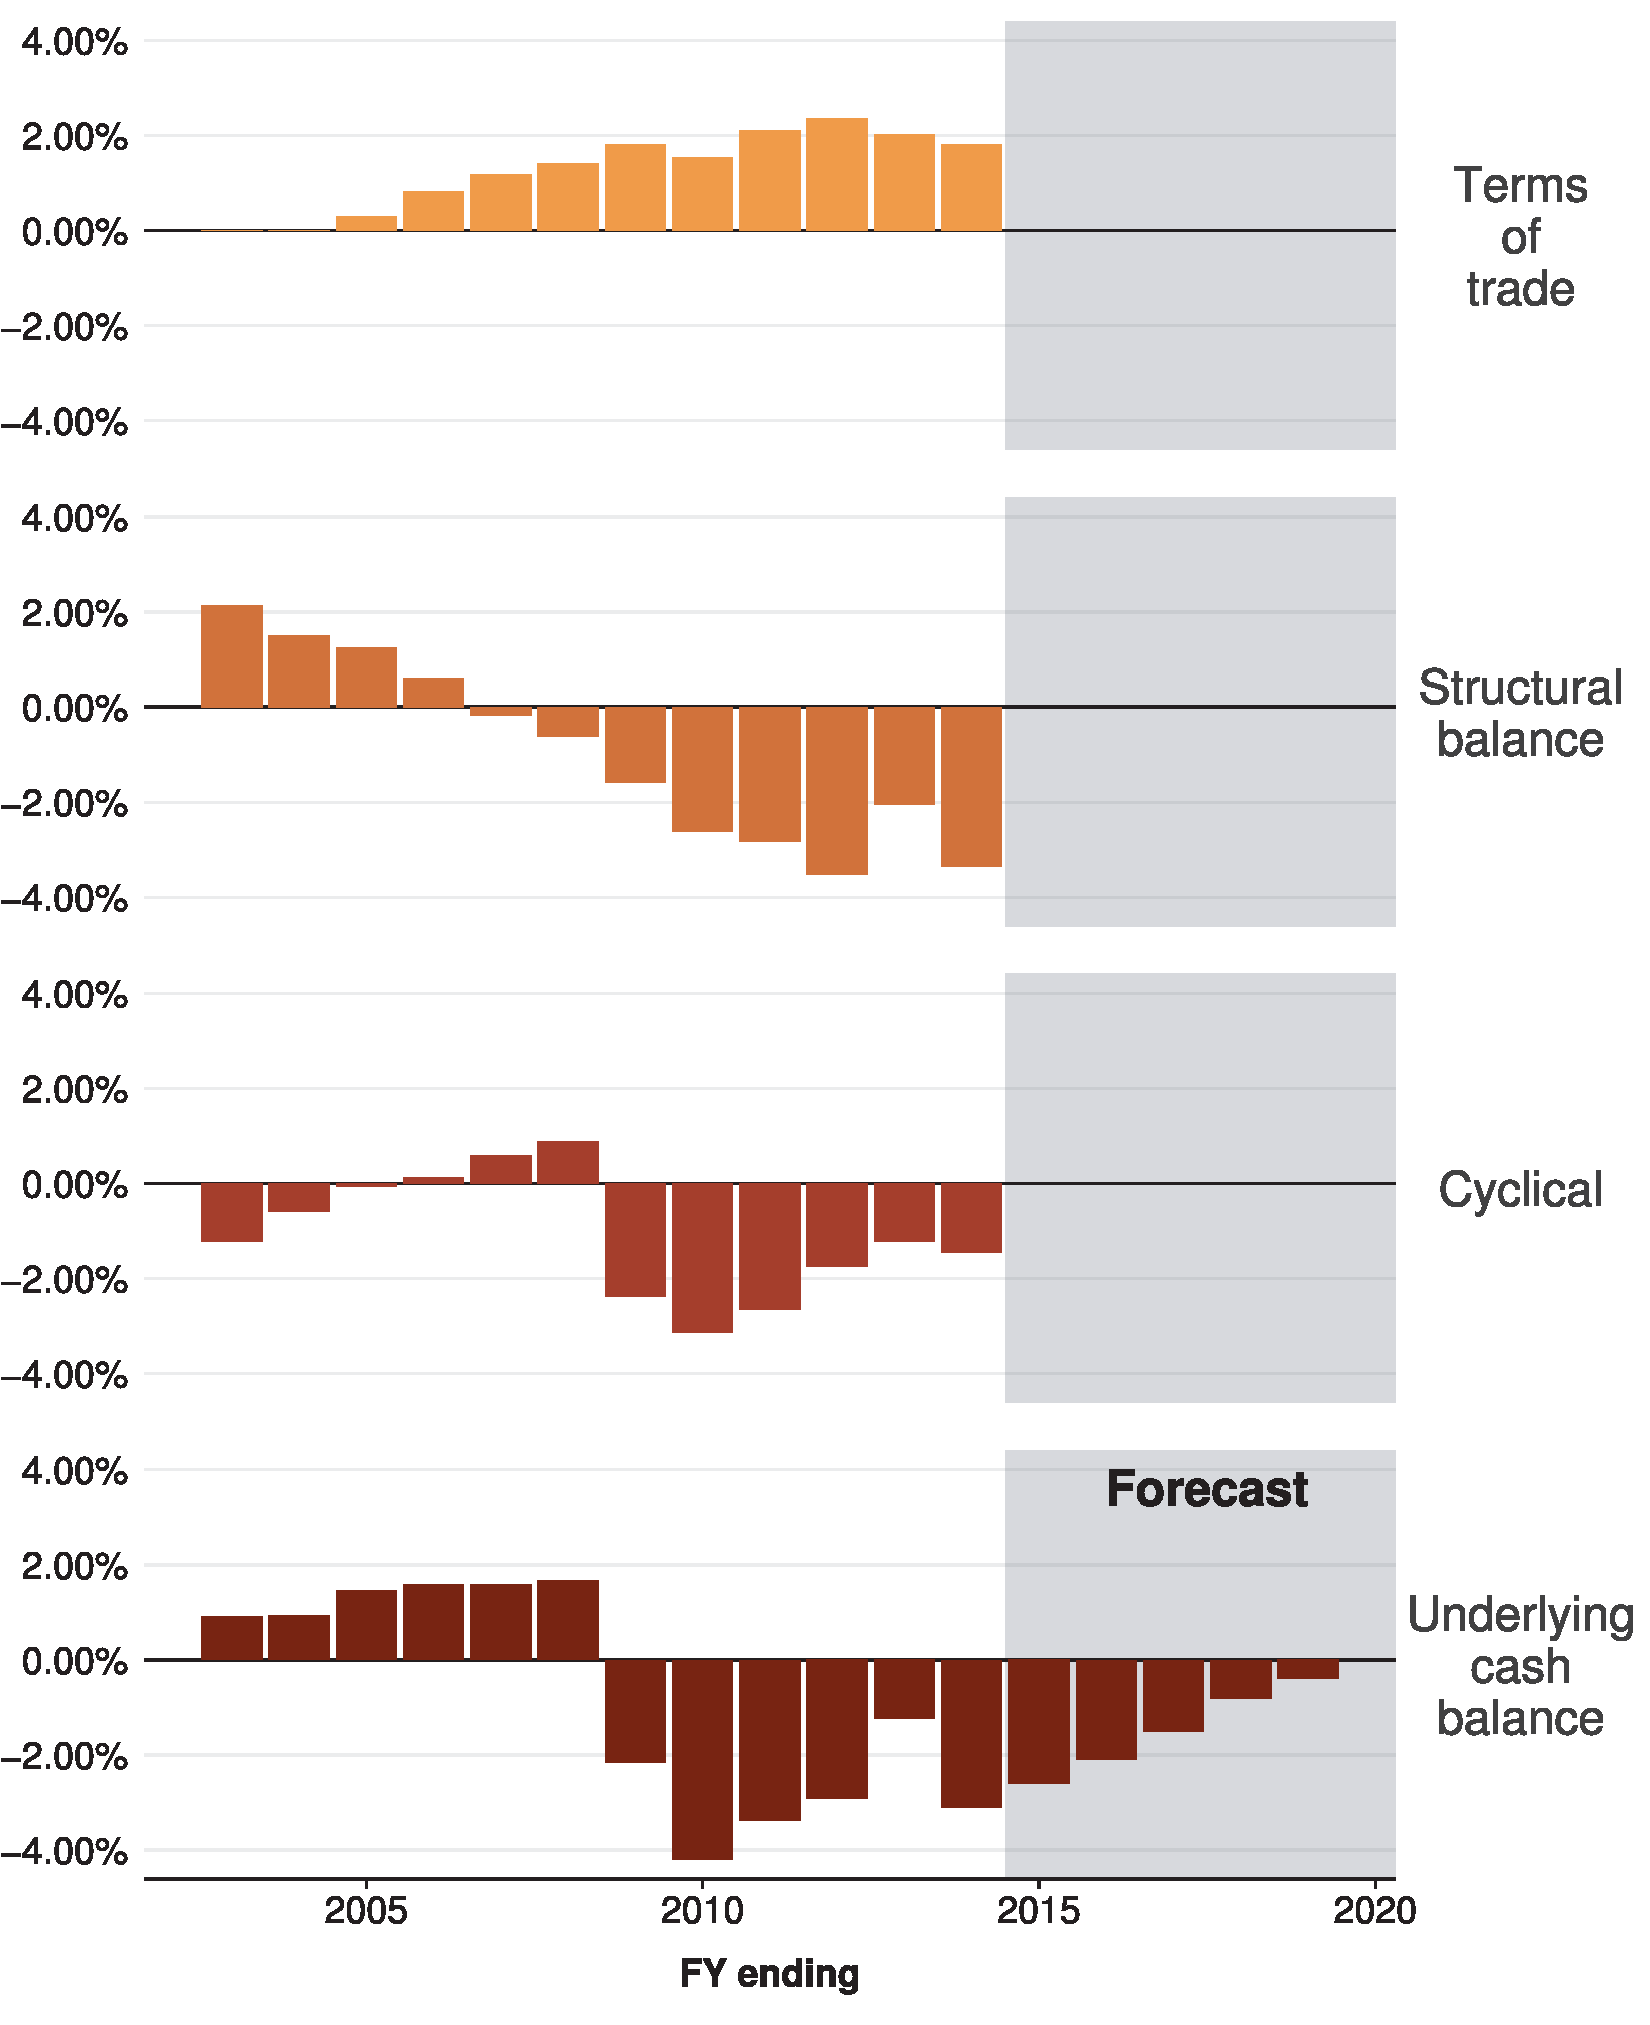
\includegraphics[width=\columnwidth]{Fiscal-challenges/figure/b5-Figure1-1.pdf}
\notes{Cash balance is equal to receipts minus payments, minus Future Fund income (under 0.25~per~cent of GDP). Stimulus is treated as a cyclical impact; changes in company tax from the decade average due to depreciation are treated as a cyclical impact. The depreciation rate is assumed to be 15~per~cent. Terms of trade baseline is 2002-03.}

\source{\textcite{MinifieCherastidthamMullerworthEtAl2013}; Grattan analysis.}
\vspace{0.075\textheight}
\end{figure}

Both higher spending and lower revenue caused these headline and structural deficits. Commonwealth revenues fell sharply during the GFC but steadily rose after 2010-11 (\Vref{fig:FISCAL-2}). Yet policy changes did not cause this rise. The Abbott Government’s Temporary Budget Repair Levy boosted revenues by about \$1 billion a year over three years, and reindexing the fuel excise in line with inflation will raise \$1 billion in 2017-18. But at the same time, the Government cut off revenue streams by abolishing the carbon and mining taxes. These were forecast to raise \$2.9 billion and \$1.1 billion respectively in 2014-15.\footcite[][55]{Treasury2013-PEFO}  

\begin{figure}[!h]
% increase the margin by -2cm, 
% oneside otherwise the caption will intrude the wrong way
\captionsetup{margin={0cm,-1.5cm}, oneside, singlelinecheck=false}
\captionwithunits{Commonwealth revenues fell while expenditures remained high\label{fig:FISCAL-2}}%
{Commonwealth revenue and expenditure as percentage of nominal GDP}
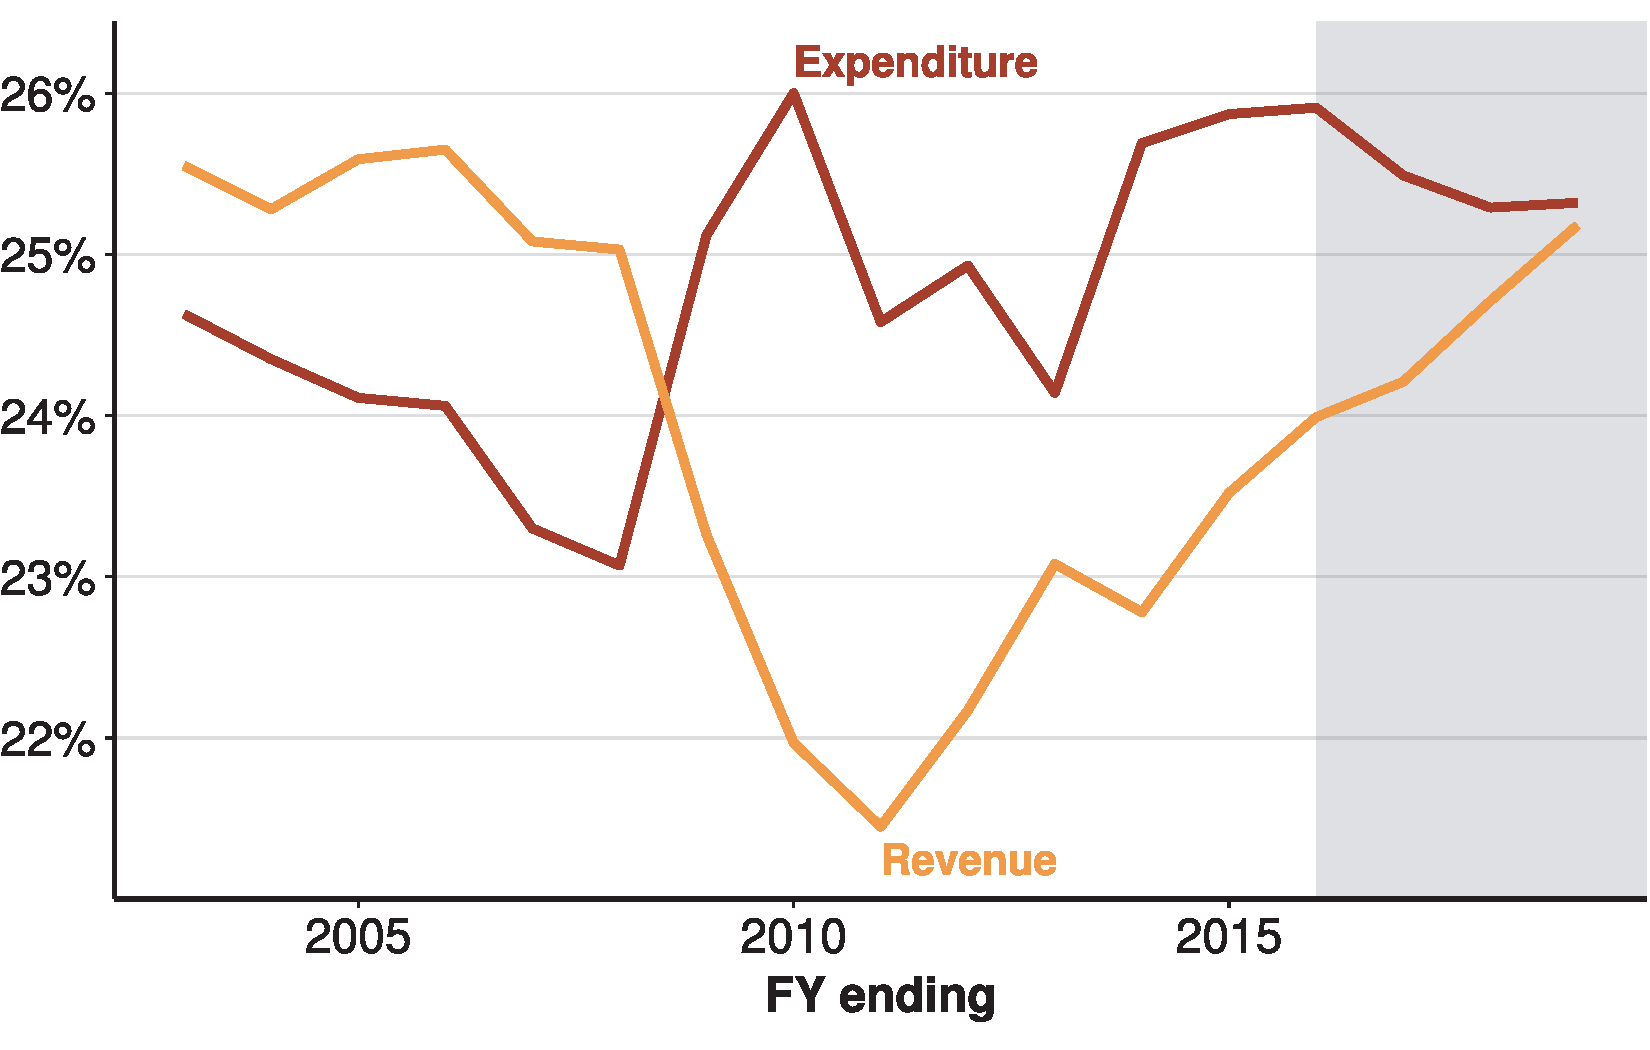
\includegraphics[width=\columnwidth]{Fiscal-challenges/figure/Figure2-1.pdf}
\captionsetup{margin = {0cm, 0cm}}
\fnotes{fig:FISCAL-2}{Revenues and expenses from the general government sector operating statement of the Commonwealth Government financial statements. Difference between revenue and spending is the net operating balance. Commonwealth “own purpose” revenues and expenses (\ie~excluding revenues from the GST, and excluding grants to the states) follow a similar pattern.}

\source{\textcite{Treasury2015BudgetPapers201516}; Grattan analysis.}
\end{figure}

Instead, most of the revenue increase over the last four years, and the increase projected over the next four years, results from existing taxes growing faster than GDP\@. Fiscal drag – growth in income tax collections as a share of wages – accounts for most of the planned improvement in the budget position (\Vref{fig:FISCAL-3}). 

\enlargethispage*{0.5\baselineskip}
When fiscal drag is not returned through periodic personal income tax cuts average tax rates for most taxpayers increase. Growth in nominal wages results in taxpayers paying their top marginal tax rate on a greater proportion of their income. %This is exacerbated for taxpayers pushed into higher tax brackets. 
Middle-income earners are particularly hurt. \Vref{fig:FISCAL-4} shows that on the wages growth projected in the 2015-16 budget, average tax rates for people in middle-income groups will increase by between 1.5~and 2.5~percentage points. A person in the sixth income decile, earning \$50,000 a year, with an average tax rate of 17.1~per cent in 2015 will pay 19.1~per cent in 2019. Such higher marginal tax rates can significantly affect incentives to participate in the workforce, particularly for women with children in childcare.\footcites[][11--12]{ProductivityCommission2015-Childcare}[][42--43]{DaleyMcGannonGinnivan2012}

\begin{figure}[hbp]
\captionwithunits{Bracket creep will increase average tax rates most for middle income earners\label{fig:FISCAL-4}}%
{Percentage point increase in average tax rates 2015 to 2019}
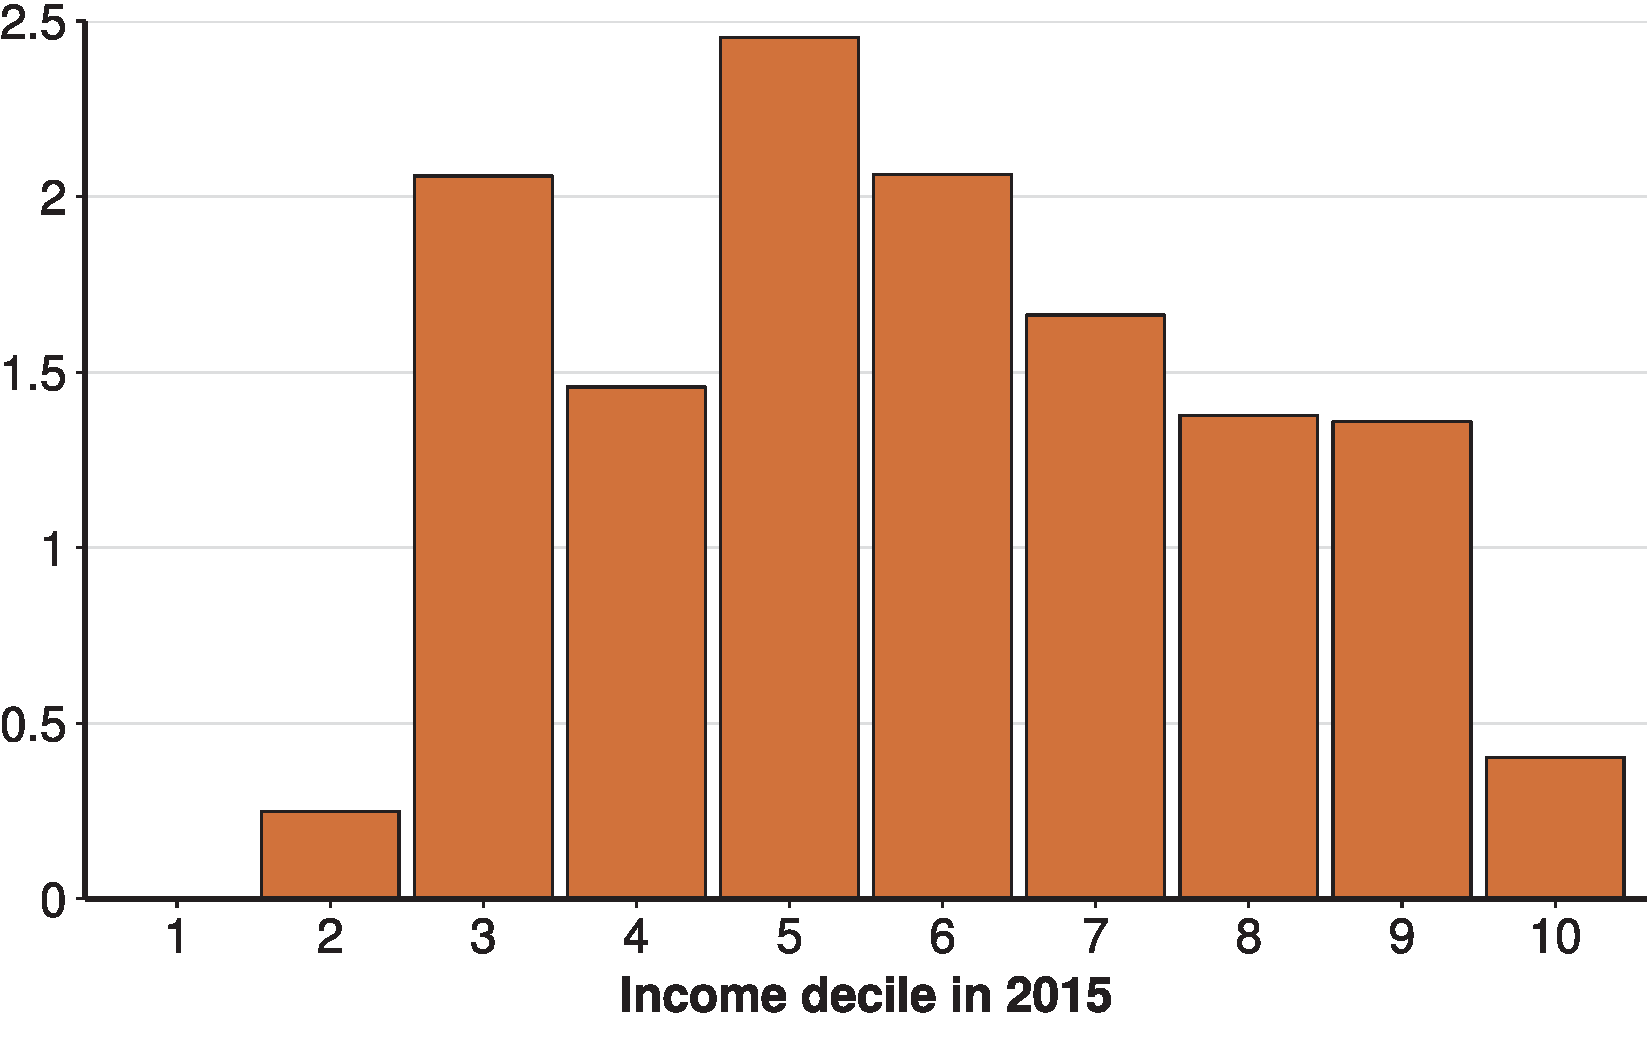
\includegraphics[width=\columnwidth]{Fiscal-challenges/figure/Figure4-1.pdf}
\source{\textcites{Treasury2015BudgetPapers201516}{ATO2015SampleFile1213}.}
\end{figure}

On the \textbf{spending} side, the Commonwealth’s stimulus package increased spending during the GFC\@. That was meant to be a one-off boost to the economy, yet since then spending has been maintained at these higher levels. Social security and welfare spending contributed about a third of the growth in spending over the decade. Growing Age Pension payments are the biggest contributor, but health, education and general public services, all of which grew faster than GDP,\footcites[][7--8]{PBO2013}[][20--23]{DaleyWoodWeidmannEtAl2014}  also increased significantly.\enlargethispage*{1\baselineskip} 
\makeatletter\@openrightfalse

In contrast, over the next four years outlays are forecast to grow slower than GDP\@. But explicit policy measures only explain some of this slower spending growth. Spending measures introduced in the Government’s 2014-15 Budget were projected to save \$14.2 billion in 2017-18.\footcite[][BP~No.~2, p.~47]{Treasury2015BudgetPapers201516}  Of these, \$5.9 billion have been passed, \$5.8 billion are stalled in the Senate (but are included in the budget projections)\footcite{PBO2015f}  and a further \$2.5~billion have been abandoned.\footnote{Grattan estimates based on major measures that have been reversed including proposal to index social security benefits to CPI, Medicare co-payments and the 6 month waiting period for Newstart Allowance.}  The Government has booked another \$2.3 billion in savings in the 2015-16 Budget. If all the measures passed, they would only restrain spending growth by about 0.8~per~cent a year.  Even on these forecasts, spending will remain a larger share of the economy than at any point between 2003 and 2008 (\Cref{fig:FISCAL-2}). 
% \begin{figure*}
% \captionwithunits{Fiscal drag is doing most of budget repair work\label{fig:FISCAL-3}}%
% {Change in budget position from 2014-15 to 2018-19, \$\,billions}

\cleardoubleevenemptypage
% \twopagepicture{t}{l}{Fiscal-challenges/figure/Figure3-1.pdf}{Fiscal drag is doing most of budget repair work\label{fig:FISCAL-3}}{Change in budget position from 2014-15 to 2018-19, \$\,billions}{fig:FISCAL-3}{\textcite{Treasury2015BudgetPapers201516}; Grattan analysis.}
\begin{figure}
\captionwithunits{Fiscal drag is doing most of budget repair work\label{fig:FISCAL-3}}{Change in budget position from 2014-15 to 2018-19, \$\,billions}
\includegraphics[width=1\linewidth]{Fiscal-challenges/figure/LeftWaterfallCropperForXeLaTeX.pdf}
\source{\textcite{Treasury2015BudgetPapers201516}; Grattan analysis.}
\end{figure}

\begin{figure}
\caption*{\null}
\includegraphics[width=0.96\linewidth]{Fiscal-challenges/figure/RightWaterfallCropperForXeLaTeX.pdf}
\caption*{\null}
\end{figure}


% \fnotes{fig:FISCAL-3}{Budget balance is the underlying cash balance from the 2014-15 budget. Estimates of the contribution of spending and revenue (including personal income tax) growth are based on the differences between the 2018-19 forecasts of these variables and the value if they had grown at the same rate as nominal GDP from 2014-15. Personal income tax includes income and other withholding taxes, superannuation fund taxes and fringe benefits. Initial growth in deficit at nominal GDP shows impact on budget balance if spending and revenue had continued to grow at nominal GDP. Other is a balancing item and includes effects of parameters changes.}
% \source{\textcite{Treasury2015BudgetPapers201516}; Grattan analysis.}
% \end{figure*}
\FloatBarrier
\afterpage{\cleardoublepage}


\chapter{Future pressures on Commonwealth budgets}\label{chapter:FISCAL-3}
Commonwealth Government revenues will struggle over the next decade if the terms of trade continue to fall and if economic growth remains sluggish. At the same time, the budget will need to make room to fund significant new spending initiatives. 

\section{Slowing income growth and tax revenues}\label{sec:FISCAL-3-1}
Australian government revenues are strongly linked to the performance of the economy and the terms of trade. When national incomes are growing strongly, personal and corporate income tax receipts increase. About two thirds of Commonwealth Government revenues come from these volatile direct taxes.\footnote{\gao\ \textcite[][BP~No.~1, pp.~5-18]{Treasury2014-Budget-Papers-2014-15}.}  The projected slower growth in Australian living standards over the next decade is therefore a problem for Commonwealth revenue.\footcite[][vii]{HenryTaxReview2010}

In the 2000s, record terms of trade led to incomes rising quickly.\footnote{\textcite{Carmody2013}. National living standards are often measured by reference to Gross Domestic Product (GDP), which measures the volume of goods and services produced in the Australian economy. Gross National Income (GNI) measures the income earned by Australian residents. GNI differs from GDP principally because GNI captures changes in the price of exports compared to the price of imports. In periods when there are large changes in the terms of trade, GNI is arguably a more accurate reflection of living standards.}  But falling terms of trade are expected to drag on future income growth. Minerals prices are falling as past mining investments increase supply.\footcites{Stevens2013}{MinifieCherastidthamMullerworthEtAl2013}  Australia’s terms of trade are forecast to fall by 9~per~cent next year, and then stabilise.\footcite[][2--5]{Treasury2015BudgetPapers201516}   

\begin{figure}[!t]
\captionwithunits{Terms of trade added to income growth in the 2000s, but will drag in the next decade\label{fig:FISCAL-5}}%
{Average annual percentage point contribution to per capita GNI}
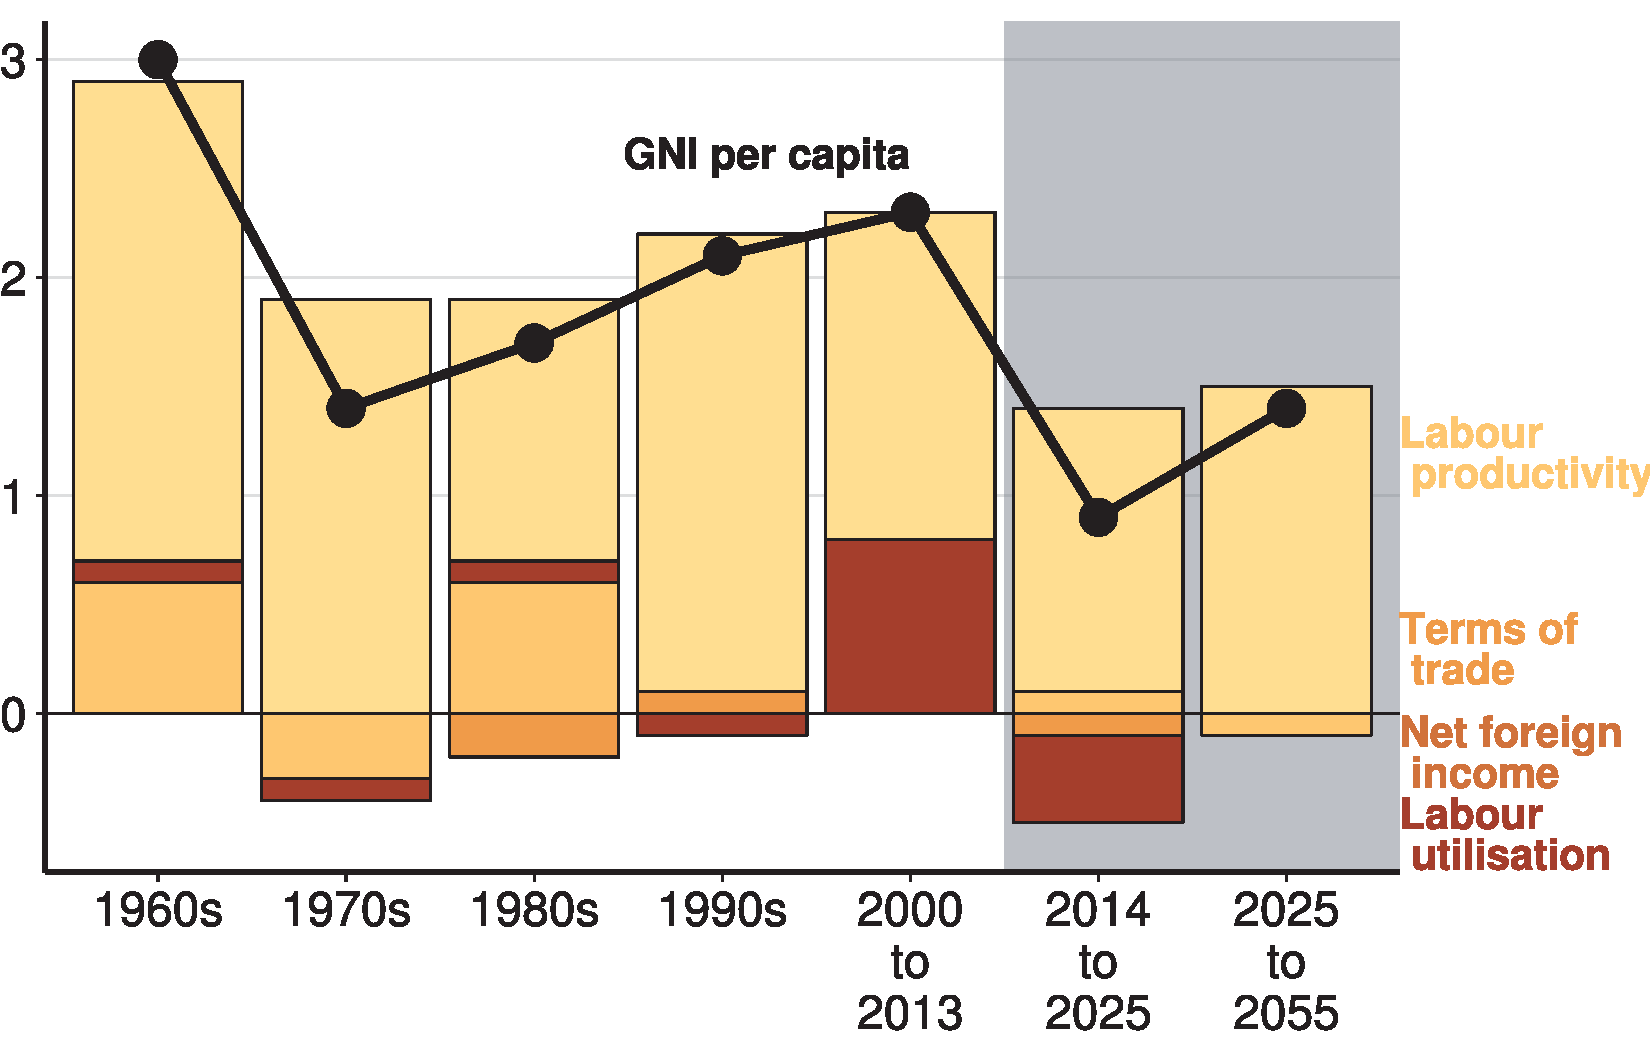
\includegraphics[width=\columnwidth]{Fiscal-challenges/figure/Figure5-1.pdf}
\notes{Assumes labour productivity for 2025-2055 is at historical average of 1.5\%.}

\source{\textcite[][33]{Hockey2015IGR}}
\end{figure} 

Other projections suggest a longer and deeper fall in the terms of trade.\footcite{Treasury2014-Budget-Papers-2014-15}  The drag on per capita incomes will be material – about 0.5~percentage points over the next decade, when the terms of trade return to long-run levels (\Vref{fig:FISCAL-5}).

Labour force participation over the next few decades will also stop boosting growth, instead dragging on growth as the baby boomer generation reaches retirement age. Treasury estimates that the labour force participation rate for people aged 15 years and over will fall from 64.6~per~cent in 2014-15 to less than 62.4~per~cent by 2054-55, as a smaller proportion of the population will be of traditional working age.  The annual impact is estimated to reduce national income growth by 0.1~percentage points, compared to the boost of 0.2 percentage points from rising participation over the past 40 years.\footcite[][pp.~ix,xi]{Hockey2015IGR}  

Labour productivity may also fall. A decline in the number of mining construction employees will reduce average labour productivity because other industries generate much less value per hour worked.\footcite{Borland2014}  This effect is likely to outweigh the ‘productivity dividend’ from past investments in the mining industry beginning production.\footcite[][12]{Commission2014} 

Over the longer-term, technological change is the main driver of higher labour productivity. But some economists warn that technology will not improve living standards as dramatically as it has done in the past.\footnote{\textcites{Gordon2012}{Cowen2011}. See \textcites{DaleyWoodWeidmannEtAl2014}{Dolamore2015} for a more detailed discussion of this literature.}  Therefore national incomes and individual living standards are likely to grow less quickly. Terms of trade are falling; participation is likely to be flat to decreasing; and there is more risk that labour productivity growth will be lower, rather than higher, than its long-term average (\Cref{fig:FISCAL-5}). As a result, Commonwealth revenues will be under pressure. Treasury has warned that Australia is highly unlikely to achieve the real rate of growth required to return the budget to surplus by relying on economic growth alone.\footcite{Parkinson2014}  

\section{Spending demands are not going away\label{sec:FISCAL-3-2}}
The Commonwealth budget will also face increasing pressures on spending from population ageing\footcite{Hockey2015IGR}  and from new policy initiatives such as the National Disability Insurance Scheme (NDIS),\index{NDIS} the Families Package, and the Direct Action policy to address climate change, and commitments to increase defence spending. Together these signature polices are likely to add more than 1~per~cent of GDP to spending over the decade.\footnote{Grattan estimates based on the forecast spending on the NDIS (\textcite{Commission2014})
and the forecast growth in childcare and defence spending above the growth in nominal GDP (\textcite{NationalCommissionAudit2014}). This does not include the cost of the Direct Action Policy because no spending estimates are available beyond the forward estimates. 
}  Funding for these commitments will need to come through some combination of increases in revenues or cuts to spending in other areas. 

The NDIS in particular will be a significant cost to the budget within the decade. The Parliamentary Budget Office (PBO) forecasts that spending on the scheme will rise to \$32~billion in 2025-26.\footcite[][5]{PBO2015} 

\section{Projections may understate the problems\label{sec:FISCAL-3-3}}
Short and medium term projections of the Commonwealth budget position, although far from rosy, may understate the challenge of budget repair. They embody optimistic assumptions about revenue and spending growth. Individually, any one of the assumptions may be defensible. Collectively, they seem unlikely. The history of the last six years is not encouraging: budget outcomes have consistently been much worse than the original projection four years earlier.

\subsection{Revenue projections}
Treasury’s projections of revenue and expenses over the four years of the forward estimates rely on income taxes rising from 11~per~cent of GDP in 2014-15 to 12.1~per~cent in 2018-19. 

The increase primarily reflects fiscal drag from rising nominal wages but also assumes a rapid recovery of capital gains tax receipts from 0.6 to 0.9~per~cent of GDP\@. On these projections, personal income tax will grow faster than the historical average for each of the next four years (\Vref{fig:FISCAL-6}).

This may be plausible if there are no changes to income tax rates and thresholds. But as average income tax burdens increase, the government is likely to face strong pressure to return some of the fiscal drag by changing the tax scales. In most years in the 2000s, governments reduced tax rates or increased tax thresholds (or both), limiting the effects of bracket creep. 

\begin{figure}[p]
\begin{minipage}{\linewidth}
\captionsetup{oneside, margin={0cm,-2.2cm}}
\captionwithunits{Personal income tax growth is projected to be higher than the last decade\label{fig:FISCAL-6}}%
{Annual growth in personal income tax revenues, historical and forecast}%
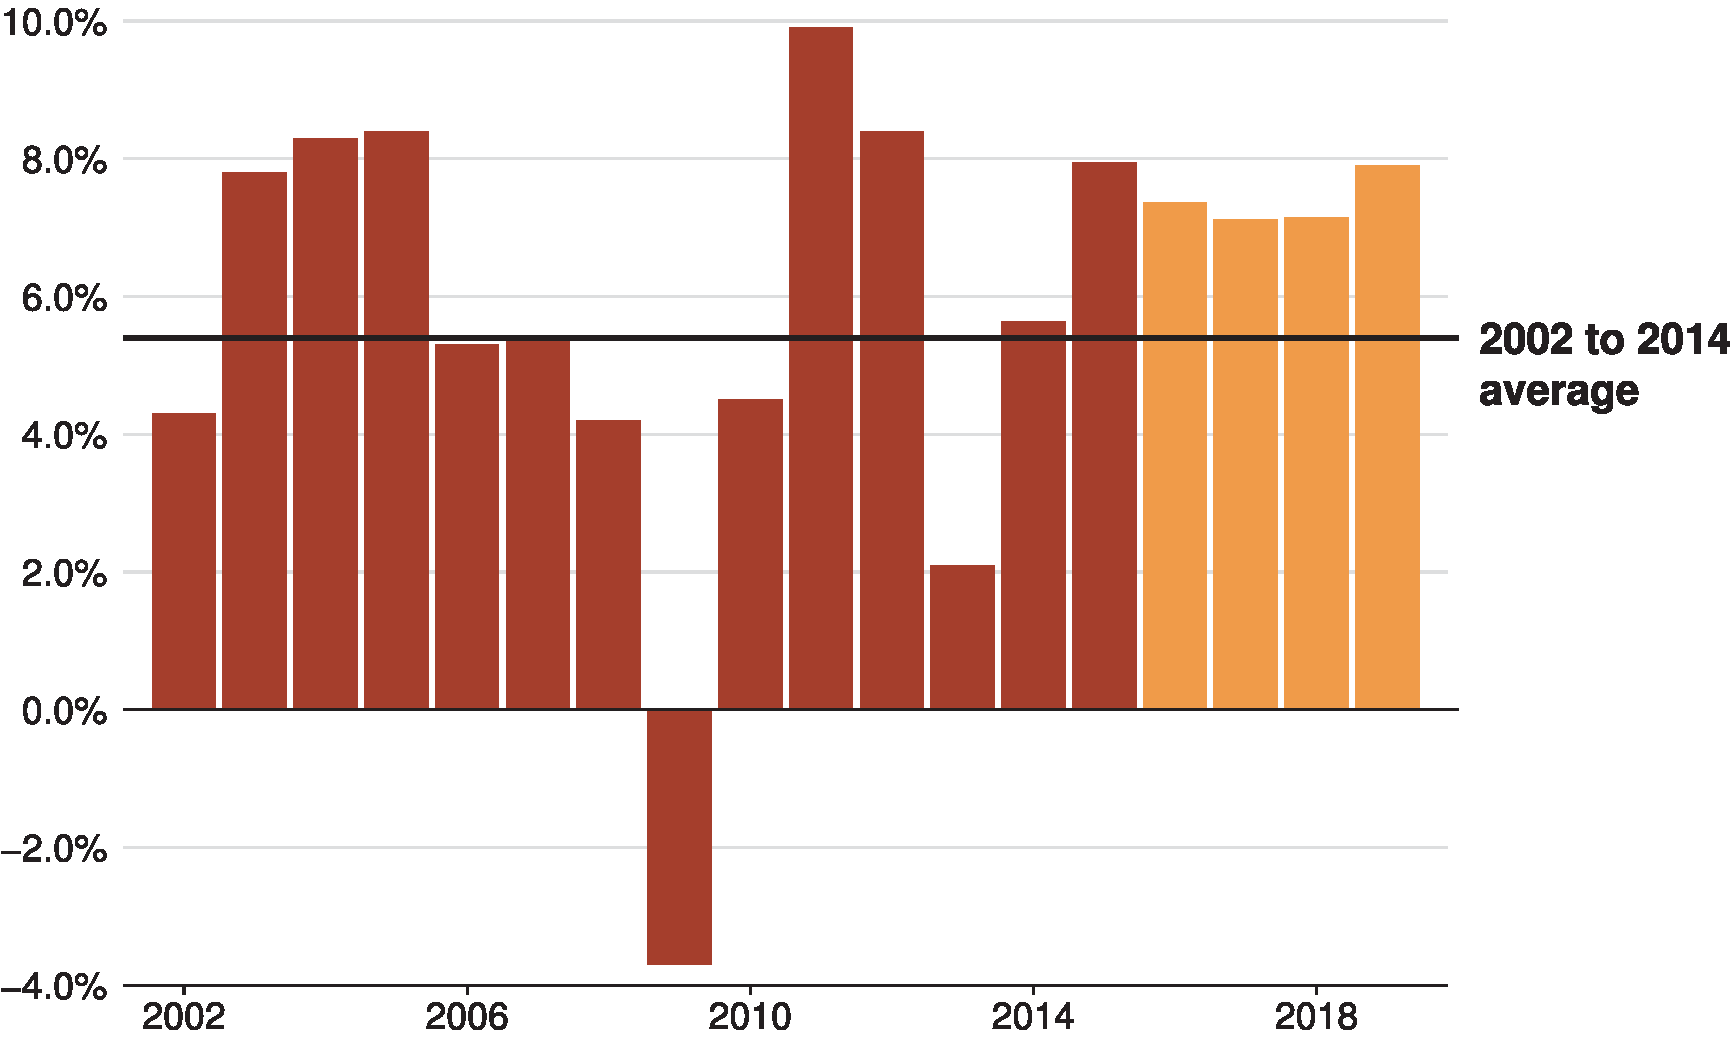
\includegraphics[width=1.05\linewidth]{Fiscal-challenges/figure/Figure6-1.pdf}
\source{\textcites{ATO2015Taxstats1213}{Treasury2015BudgetPapers201516}.}
\end{minipage}
\vfil\vspace{8pt}\vfil
\begin{minipage}{\linewidth}
\captionsetup{oneside, margin={0cm,-1.5cm}}
\captionwithunits{Terms of trade are projected to stabilise above their long-term average\label{fig:FISCAL-7}}%
{Terms of trade, 2013-14 = 100}
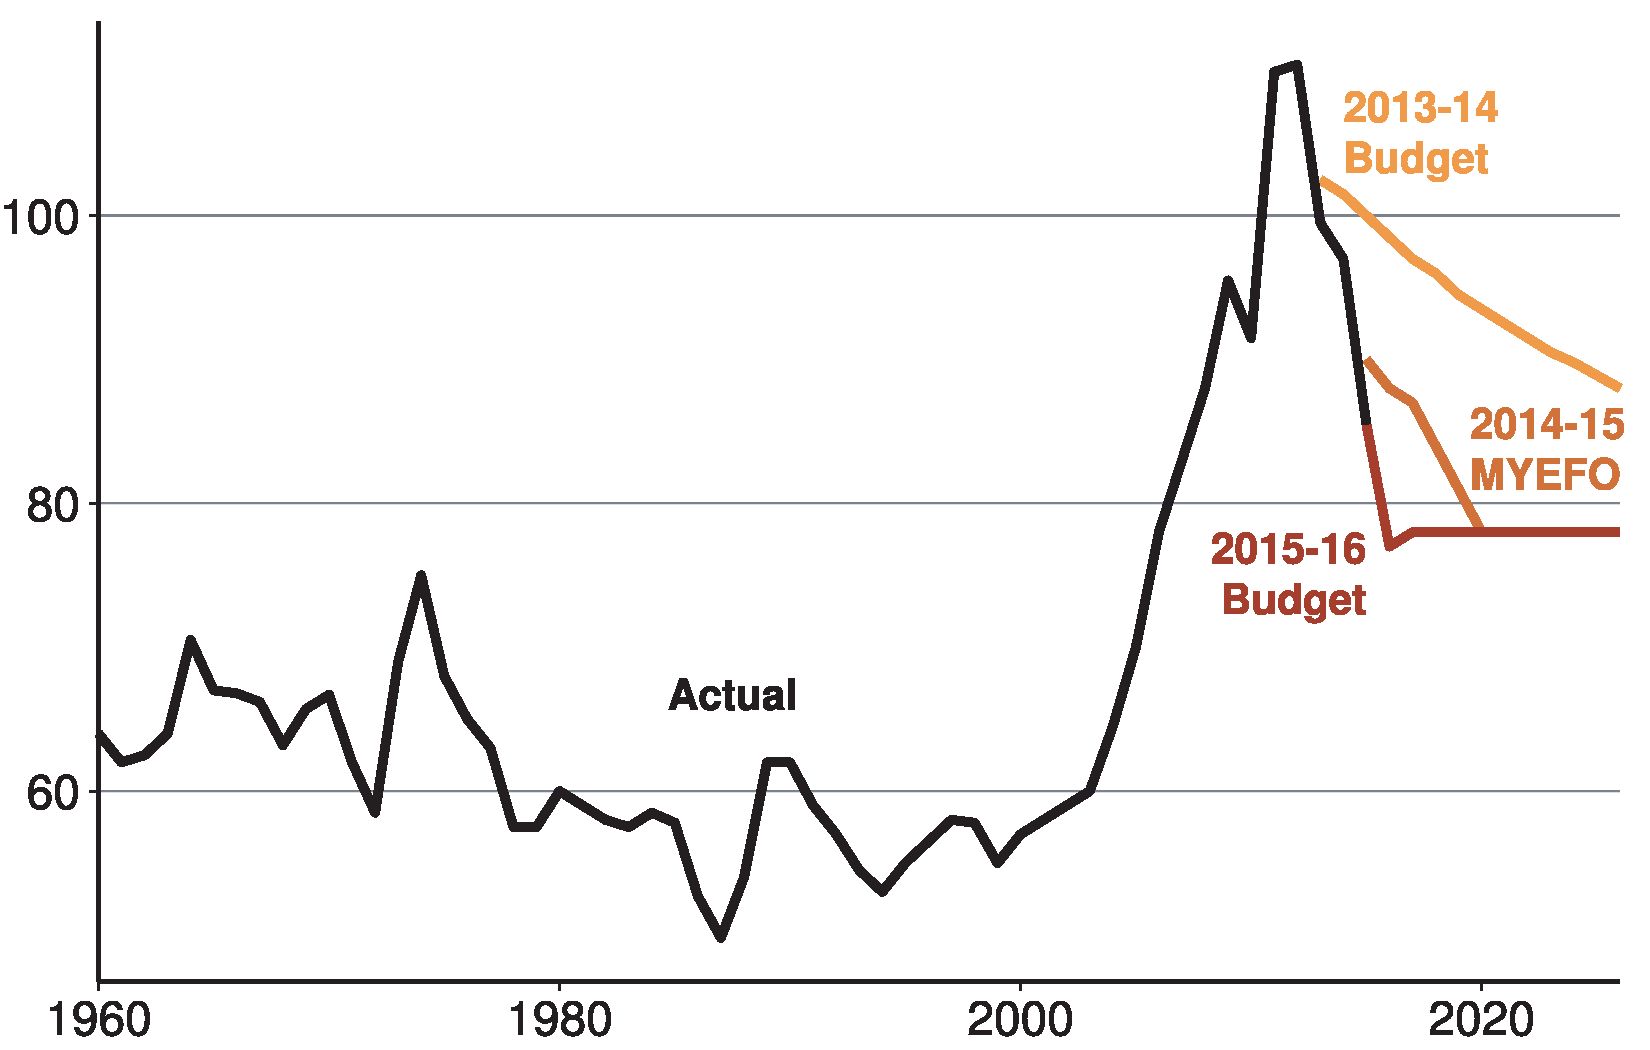
\includegraphics[width=\linewidth]{Fiscal-challenges/figure/Figure7-1.pdf}
\source{\textcite{Eslake2015}}
\end{minipage}
\end{figure}  

Other revenue projections are also optimistic. The 2015-16 budget projects that the terms of trade will fall by 9~per~cent in 2015-16 and then stabilise at a level about 50~per~cent higher than their long-run average (\Vref{fig:FISCAL-7}). However, terms of trade shocks around the world in the last few decades have typically been symmetrical. In other words, the terms of trade have tended to revert to their long-run average. \footcite[][34--35]{MinifieCherastidthamMullerworthEtAl2013} 

% \begin{figure}
% \captionwithunits{Terms of trade are projected to stabilise above their long-term average\label{fig:FISCAL-7}}%
% {Terms of trade, 2013-14 = 100}
% 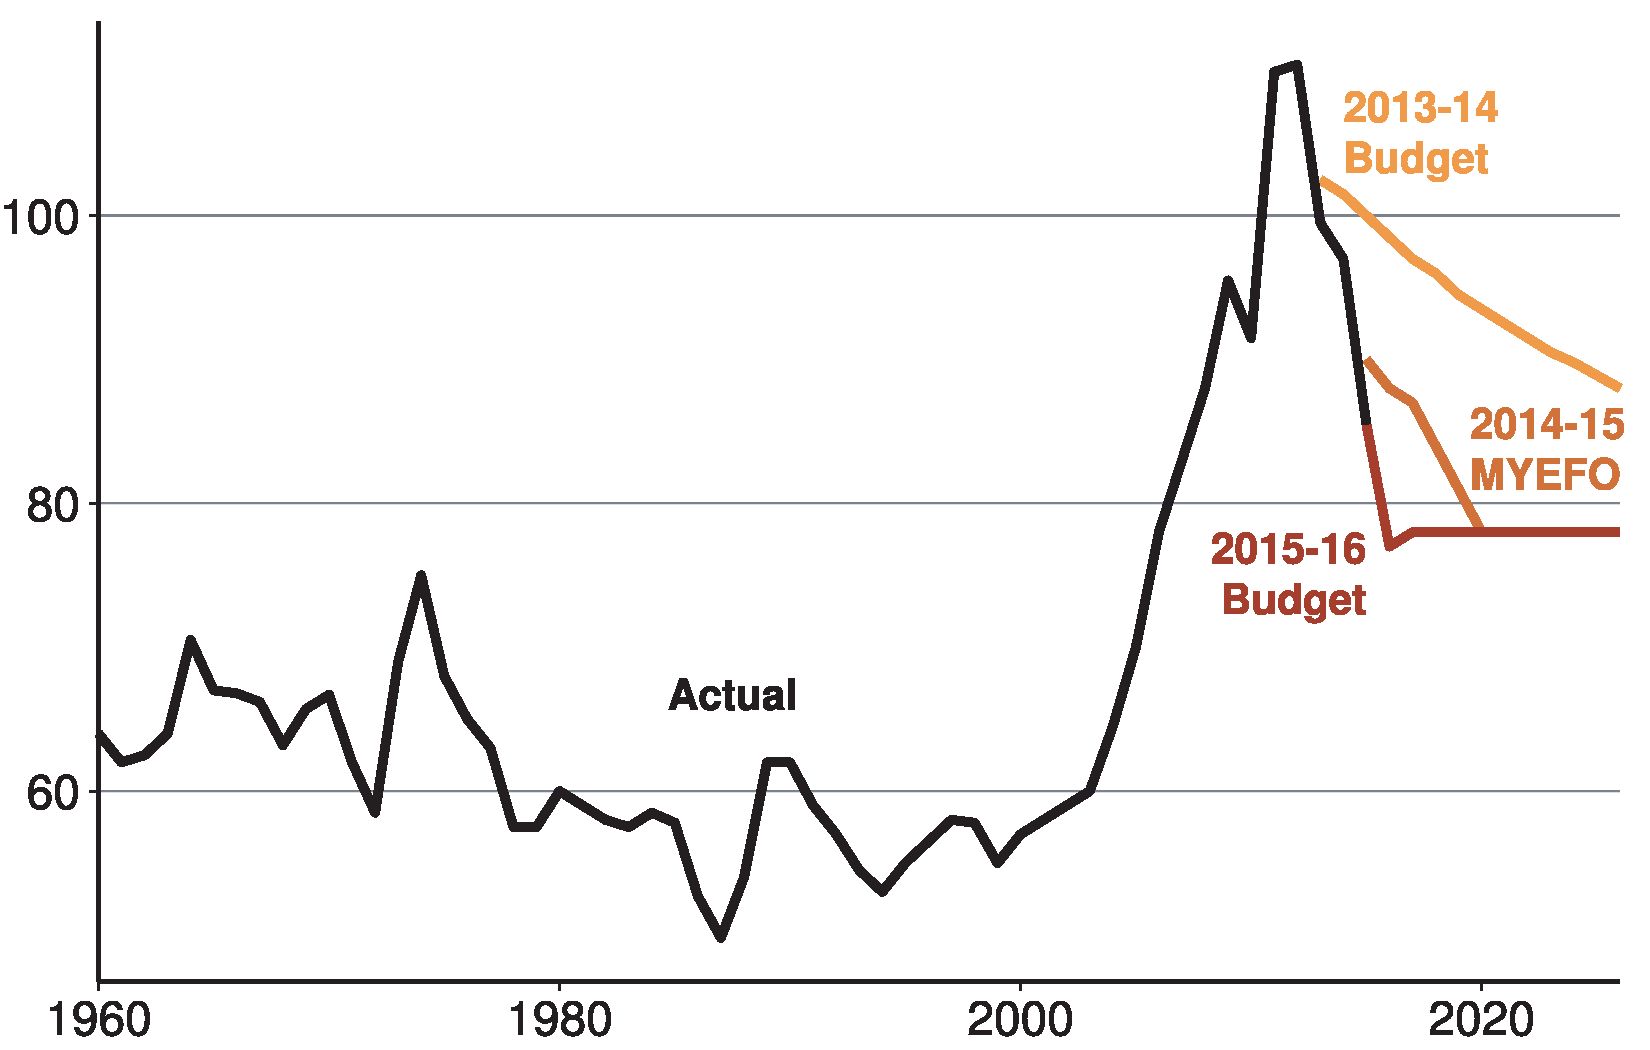
\includegraphics[width=\columnwidth]{Fiscal-challenges/figure/Figure7-1.pdf}
% \source{\textcite{Eslake2015}}
% \end{figure}

The budget also projects a healthy economic growth rate of 3.25~per~cent in 2016\nobreakdash-17 and 3.5~per~cent after that – including non-mining investment growth of 7.5~per cent in 2016\nobreakdash-17.\footcites[][1--7]{Treasury2015BudgetPapers201516}  In contrast, ABS and Reserve Bank survey data suggest non-mining investment could remain subdued for some time.\footcite[][38--44]{RBA2015a}  

These revenue projections are underpinned by an overarching assumption that by the end of the two-year estimates period the economy will return to the medium- to long-term growth rate.\footnote{\textcite{Treasury2014h}.  More precisely, the projections assume that economic activity increases to close the output gap, so if growth has been below trend, then economic growth is projected to be higher than the long run average.}

The assumption begs the question of what long-term growth rate is appropriate. Since the global financial crisis economic growth has been much slower in developed countries. In the 20 years leading up to the GFC (1988-2007), real GDP grew by an average of 2.8~per~cent a year across the OECD\@. Since 2010, the average growth rate has been just 1.6~per cent.\footnote{\gao\ \textcite{OECD2015a}.}  The IMF has warned that potential output growth rates in advanced economies are likely to remain below pre-GFC rates for at least the next five years because of the negative effects of demographics and the slow recovery in business investment.\footcite[][Chapter~3]{IMF2015b}  On this basis, it suggested Australia should expect slower growth for several years.\footcite{IMF2015} 

The longer-term prognosis is not yet clear:  it may just be a sluggish recovery, typical for a finance-induced recession, that will ultimately pass,  although the global increase in debt levels may foreshadow a lot more adjustment to come.\footcites{BailyBosworth2013}{RoxburghLundWimmerEtAl2011} Or it may reflect gloomy predictions that economic growth in coming decades will be slower than for the last few decades.\footcite[][footnote~23]{RoxburghLundWimmerEtAl2011} 

Whatever lies ahead, the overall Commonwealth budget projections look optimistic and unlikely to be realised. A PBO report concluded that the risks to the budget from economic shocks are weighted to the downside. It identified a real risk that labour productivity growth and the terms of trade will be less favourable than projected, significantly reducing tax collections.\footcite{PBO2014TrendsAustralianGovtReceipts1982to2013}  Company tax receipts could also well be lower than forecast given slower business capital expenditure  and losses carried forward from the GFC.\footcite[][38--44]{RBA2015a}

\section{Spending projections}
The Commonwealth’s spending projections also seem optimistic. They assume tight spending restraint, with government spending falling as a share of the economy (\Cref{fig:FISCAL-2}).\footcite[][5--11]{Treasury2015BudgetPapers201516}  The projections forecast spending to grow at just 2.6~per cent a year on average between 2014\nobreakdash-15 and 2025\nobreakdash-26, far below the 3.6~per~cent average growth rate of the last decade.\footcite[][5]{PBO2015}  Consistent with this spending restraint, the Commonwealth Government forecasts that spending will decline to 24.2 per cent of GDP in 2024-25, below its long term average.\footcite[][3--9]{Treasury2015BudgetPapers201516}  

Spending is forecast to be below the historical average in all program areas other than defence, as is shown in \Vref{fig:FISCAL-8}, which compares the projected growth in the Commonwealth’s largest spending programs over the next 10 years with the history of the last 10~years. 

\begin{figure}
\caption{Spending forecasts rely on lower growth in almost all major programme areas\label{fig:FISCAL-8}}%
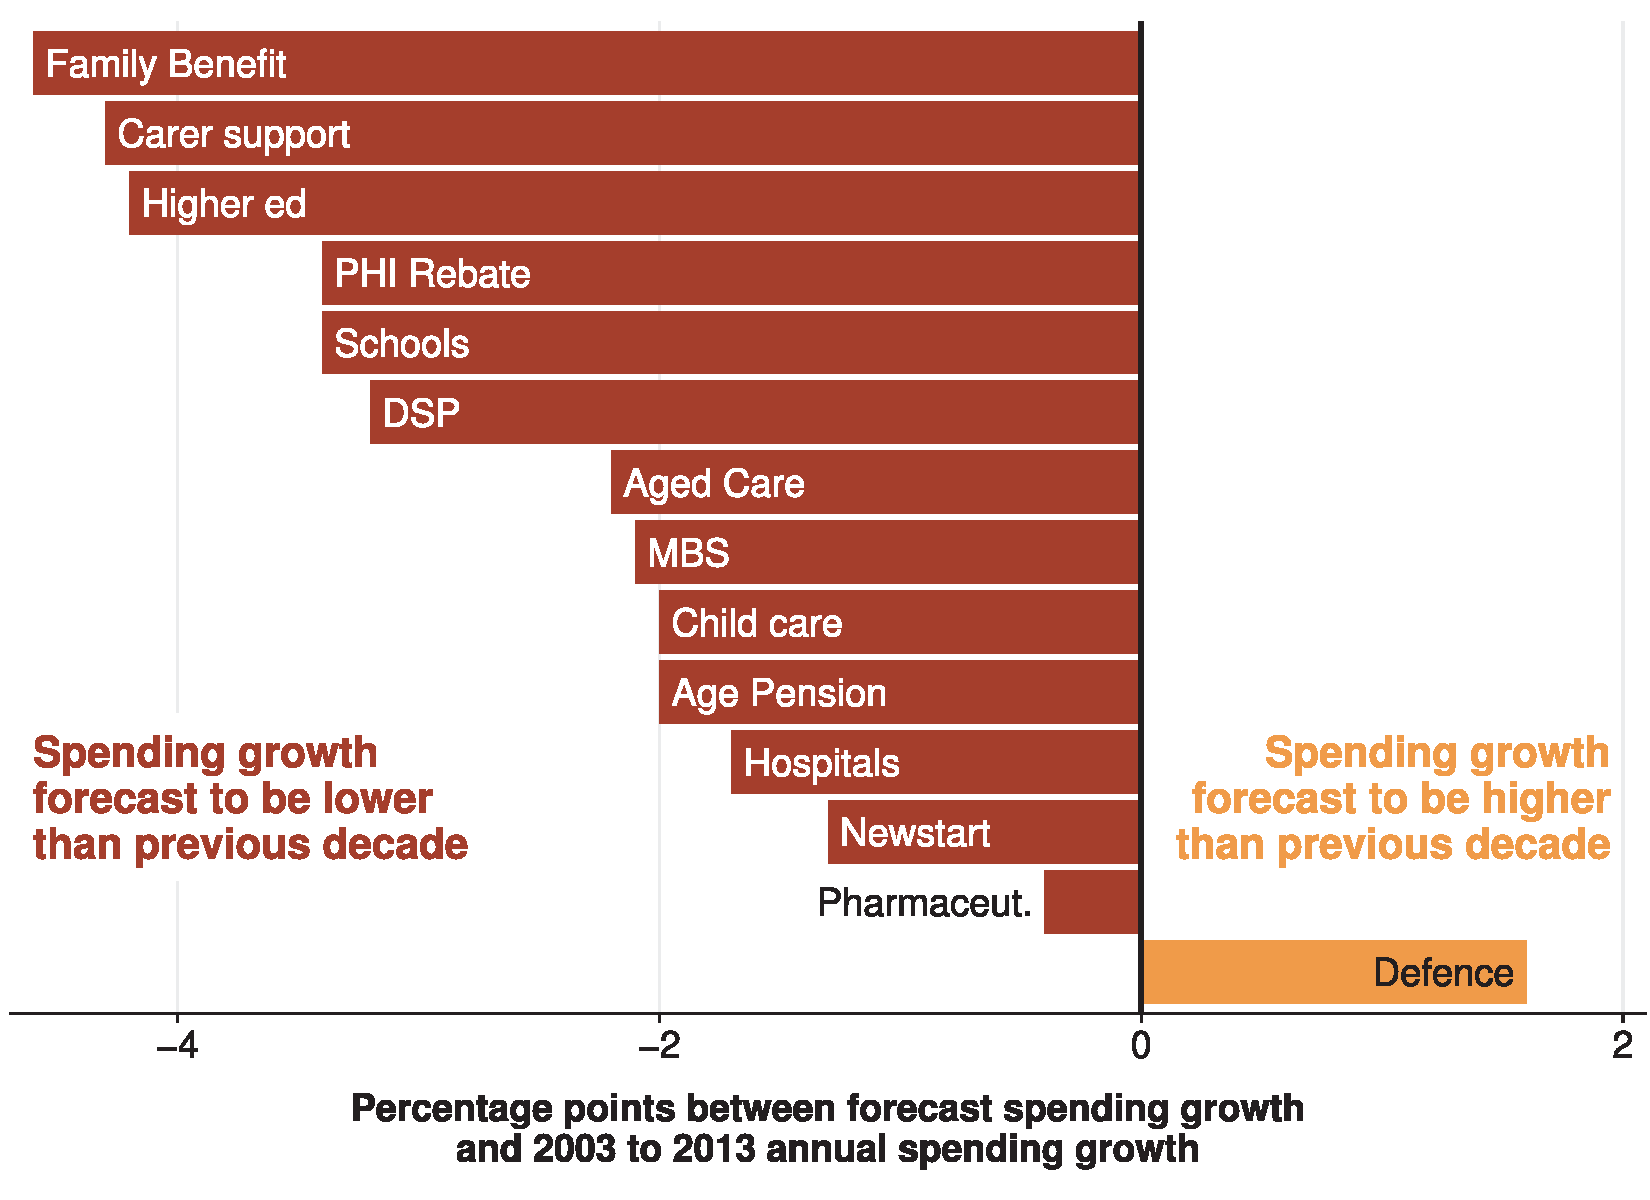
\includegraphics[width=\columnwidth]{Fiscal-challenges/figure/Figure8-altered-1.pdf}
\notes{The defence estimates do not factor in the commitment to increase defence spending to 2~per~cent of GDP by 2023-24. Rather they are based on the long-term funding commitments made in previous Defence White Papers and government announcements.}

\source{\textcite{PBO2014}}
\end{figure}

Some of these estimates seem improbable. For example, it seems unlikely that spending on demand-driven programs such as the \textbf{Medicare Benefits Schedule} will moderate without significant policy changes. The PBO attributes the strong historical growth in Medicare payments to policies (such as the Bulk Billing Incentive and the Extended Medicare Safety Net) that have made Medicare services more attractive or accessible. New policy measures such as the freeze in Medicare scheduled fees are forecast to produce lower growth. Yet for more than 20 years the ageing of the population, medical science and technology improvements and rising expectations of the health system have put relentless pressure on the health budget.\footcite{Daley2014}  These pressures will not abate, and the forecasts almost certainly understate them.

The decline in spending growth for hospitals and schools may be credible given the decision in the 2014-15 Budget to limit spending increases to inflation and population growth. This of course does not mean that spending growth will decline in these program areas – merely that the states will have to bear all of the cost of real per capita growth.\DEVIATION{Who knows?}

The 2015-16 budget assumes even tighter spending growth than have previous budgets. Except for welfare spending, mainly driven by the NDIS, no category is expected to grow materially faster than inflation.\footcite[][BP No.~1, pp.~5--11]{Treasury2015BudgetPapers201516}  

In other programs, lower forecast growth rates are tied to measures from the 2014-15 and 2015-16 Budgets that are unlikely to be passed by the Senate. Therefore spending on the Carers Payment, higher education and Newstart benefits is likely to be more than forecast\DEVIATION{}. Even the forecast growth in defence spending – the only program area where spending is forecast to grow faster than in the last decade – does not put Australia on a path to spend 2~per~cent of GDP on defence by 2023-24 as the Government has promised.\footnote{See: \textcite[][1]{Defence2014}.} 


Spending projections also assume there will be no new spending initiatives promised at elections or in response to natural disasters or community demands for more assistance to the disadvantaged. Experience over the last decade suggests that such spending restraint will be difficult (\Vref{box:FISCAL-1}).

Given all the number of things that need to go right, moderating spending growth to 24.2~per~cent of GDP in 2024-25 seems extremely unlikely without further explicit budget measures to cut expenditure.

\subsection{Experience of budget forecasts and outcomes}\label{subsubsec:3-3-3}
The government’s fiscal strategy relies heavily on these optimistic projections. The measures introduced in this year’s budget will make no net improvement to the budget position in 2018-19 (\Cref{fig:FISCAL-3}). The government justifies its inaction by saying that the projections suggest it is on a “clear and credible path back to surplus.”  But projections over the past five years have consistently overestimated the position of the budget four years out (\Vref{fig:FISCAL-9}). 

\begin{figure}
\captionwithunits{Budget forecasts have persistently missed the mark\label{fig:FISCAL-9}}%
{Underlying cash balance, forecasts and actual, coloured by year of forecast}
% 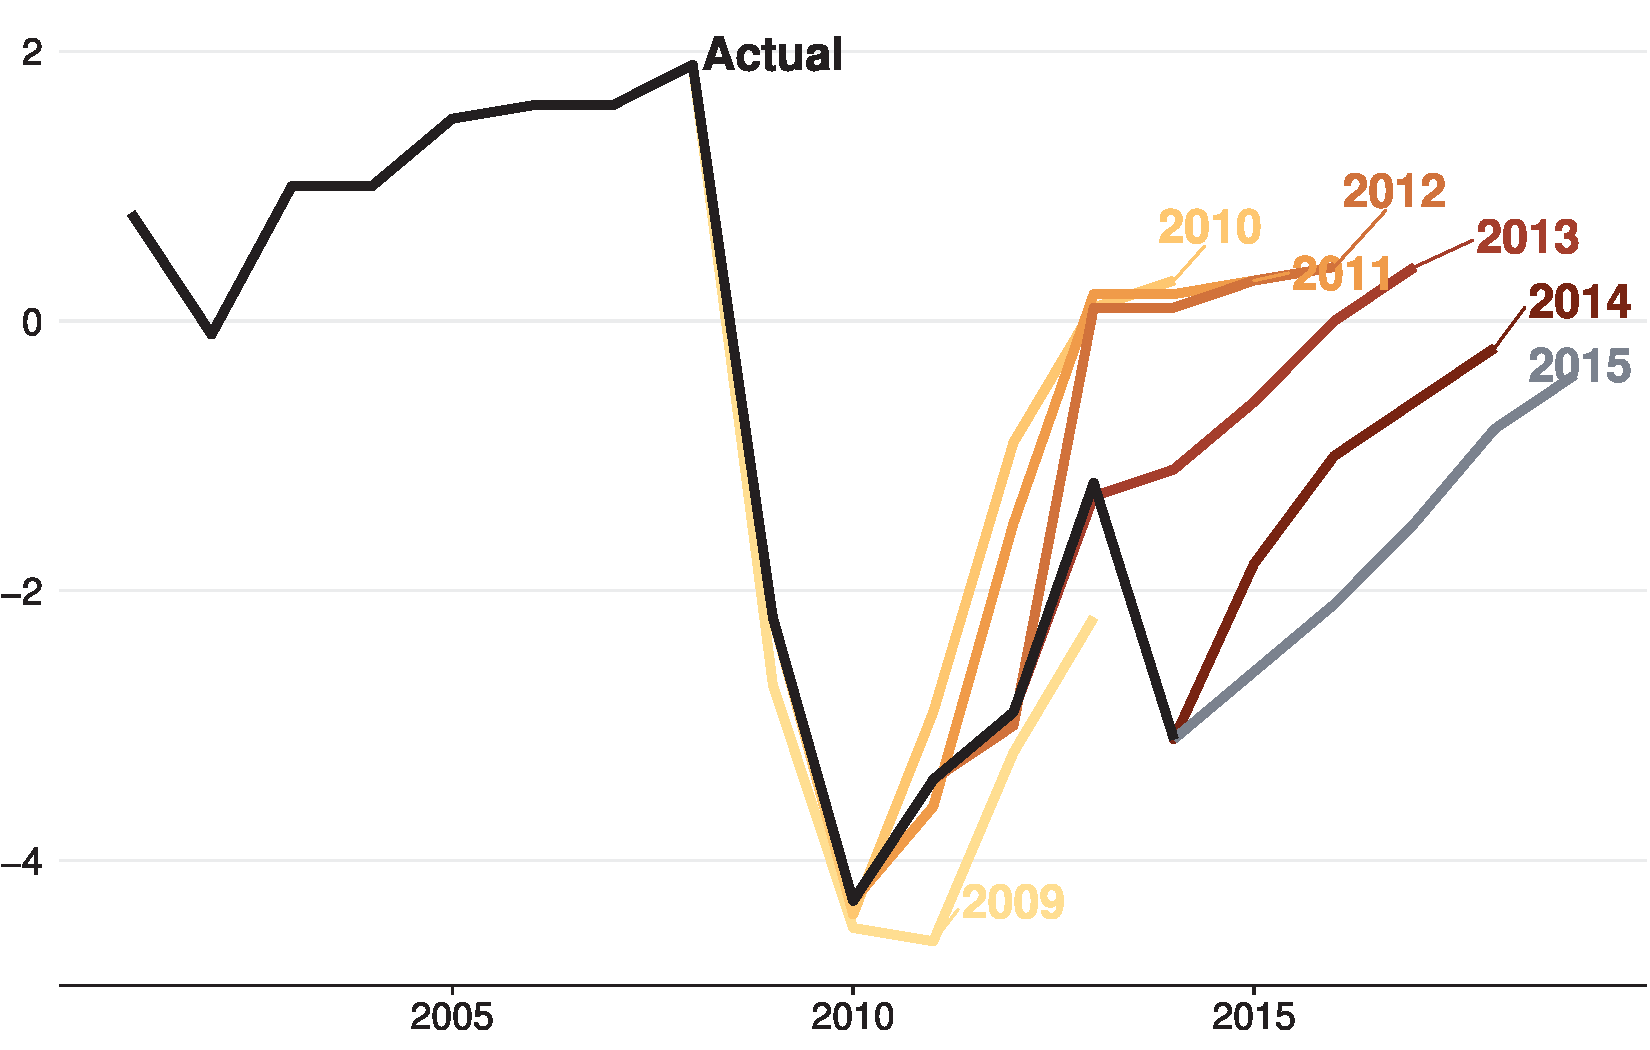
\includegraphics[width=\columnwidth]{Fiscal-challenges/figure/Figure9a-1.pdf}
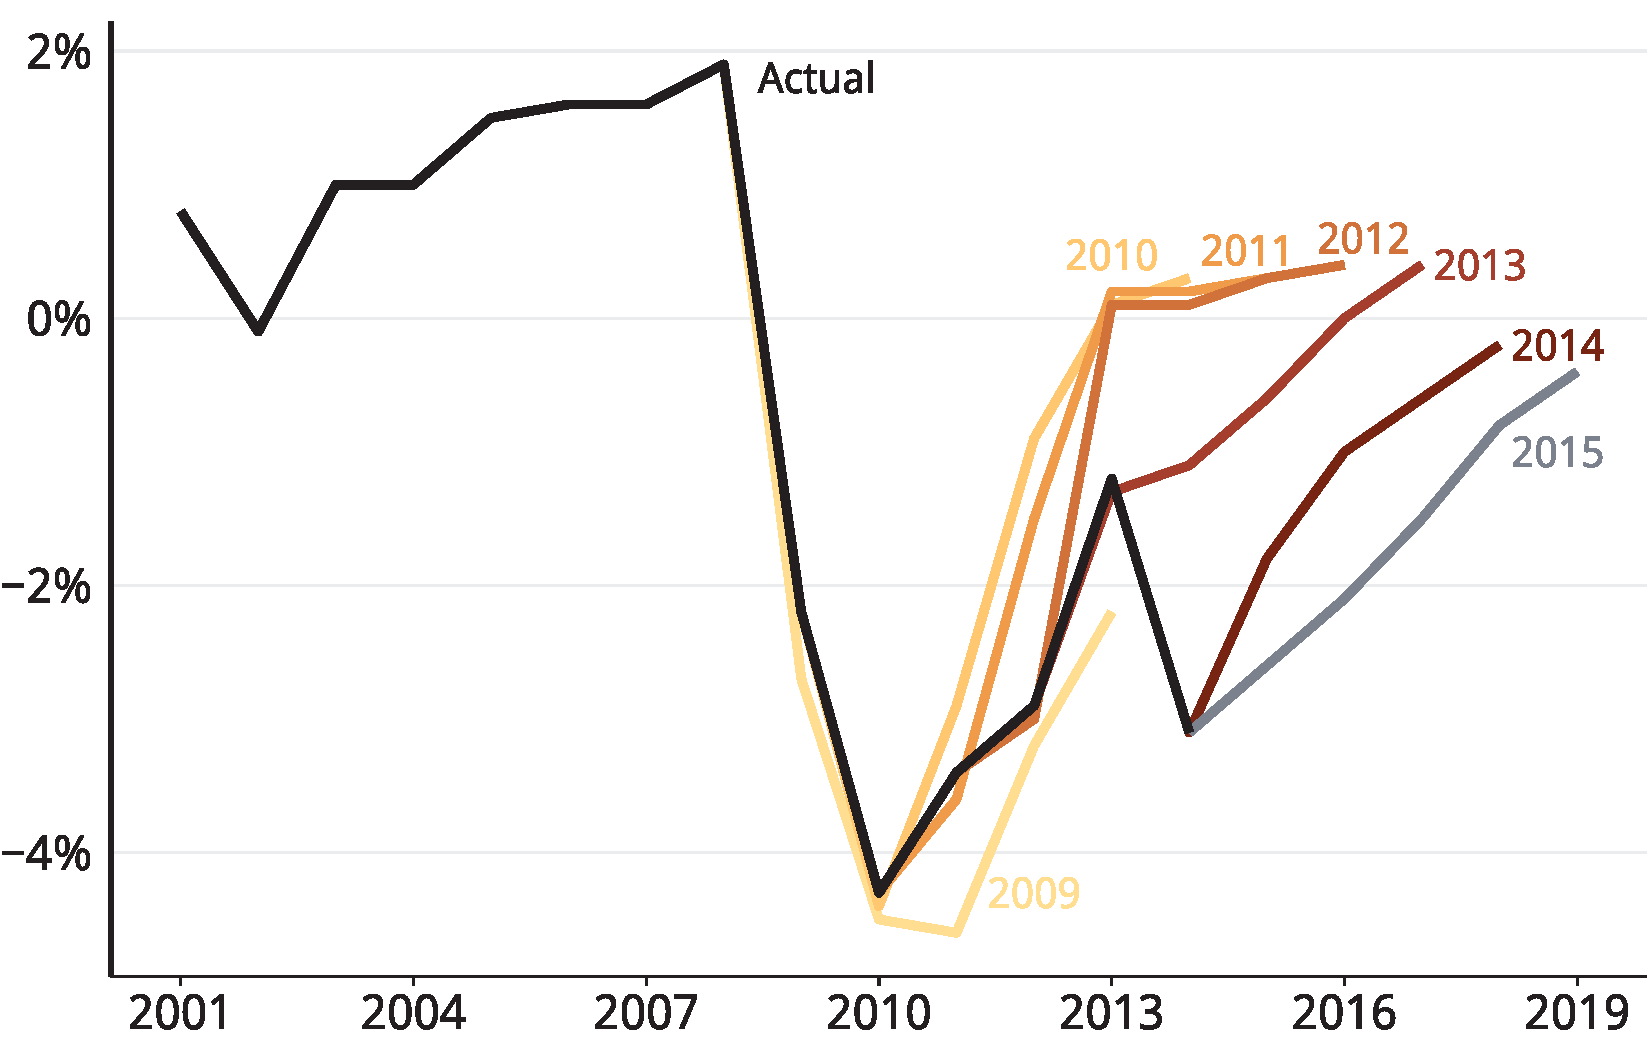
\includegraphics[width=\linewidth]{b5-figure/FISCAL-Figure9a-1.pdf}
\source{Commonwealth Budget papers 2009-10 to 2015-16}
\end{figure}

\Vref{fig:FISCAL-10} shows why. In the years leading up to the global financial crisis, forecasters underestimated the budget position by failing to anticipate the large spending and tax bonuses delivered in response to the crisis. These spending and revenue policy measures generated cumulative forecast errors in excess of six per cent of GDP for 2009.  They were offset by higher revenues due to the unexpected increases in mining prices from 2006-2009.

\begin{figure}
\captionwithunits{Budget outcomes have disappointed due to spending decisions and revenue shocks\label{fig:FISCAL-10}}%
{Cumulative change over 4 years to budget balance projection as percentage of GDP}
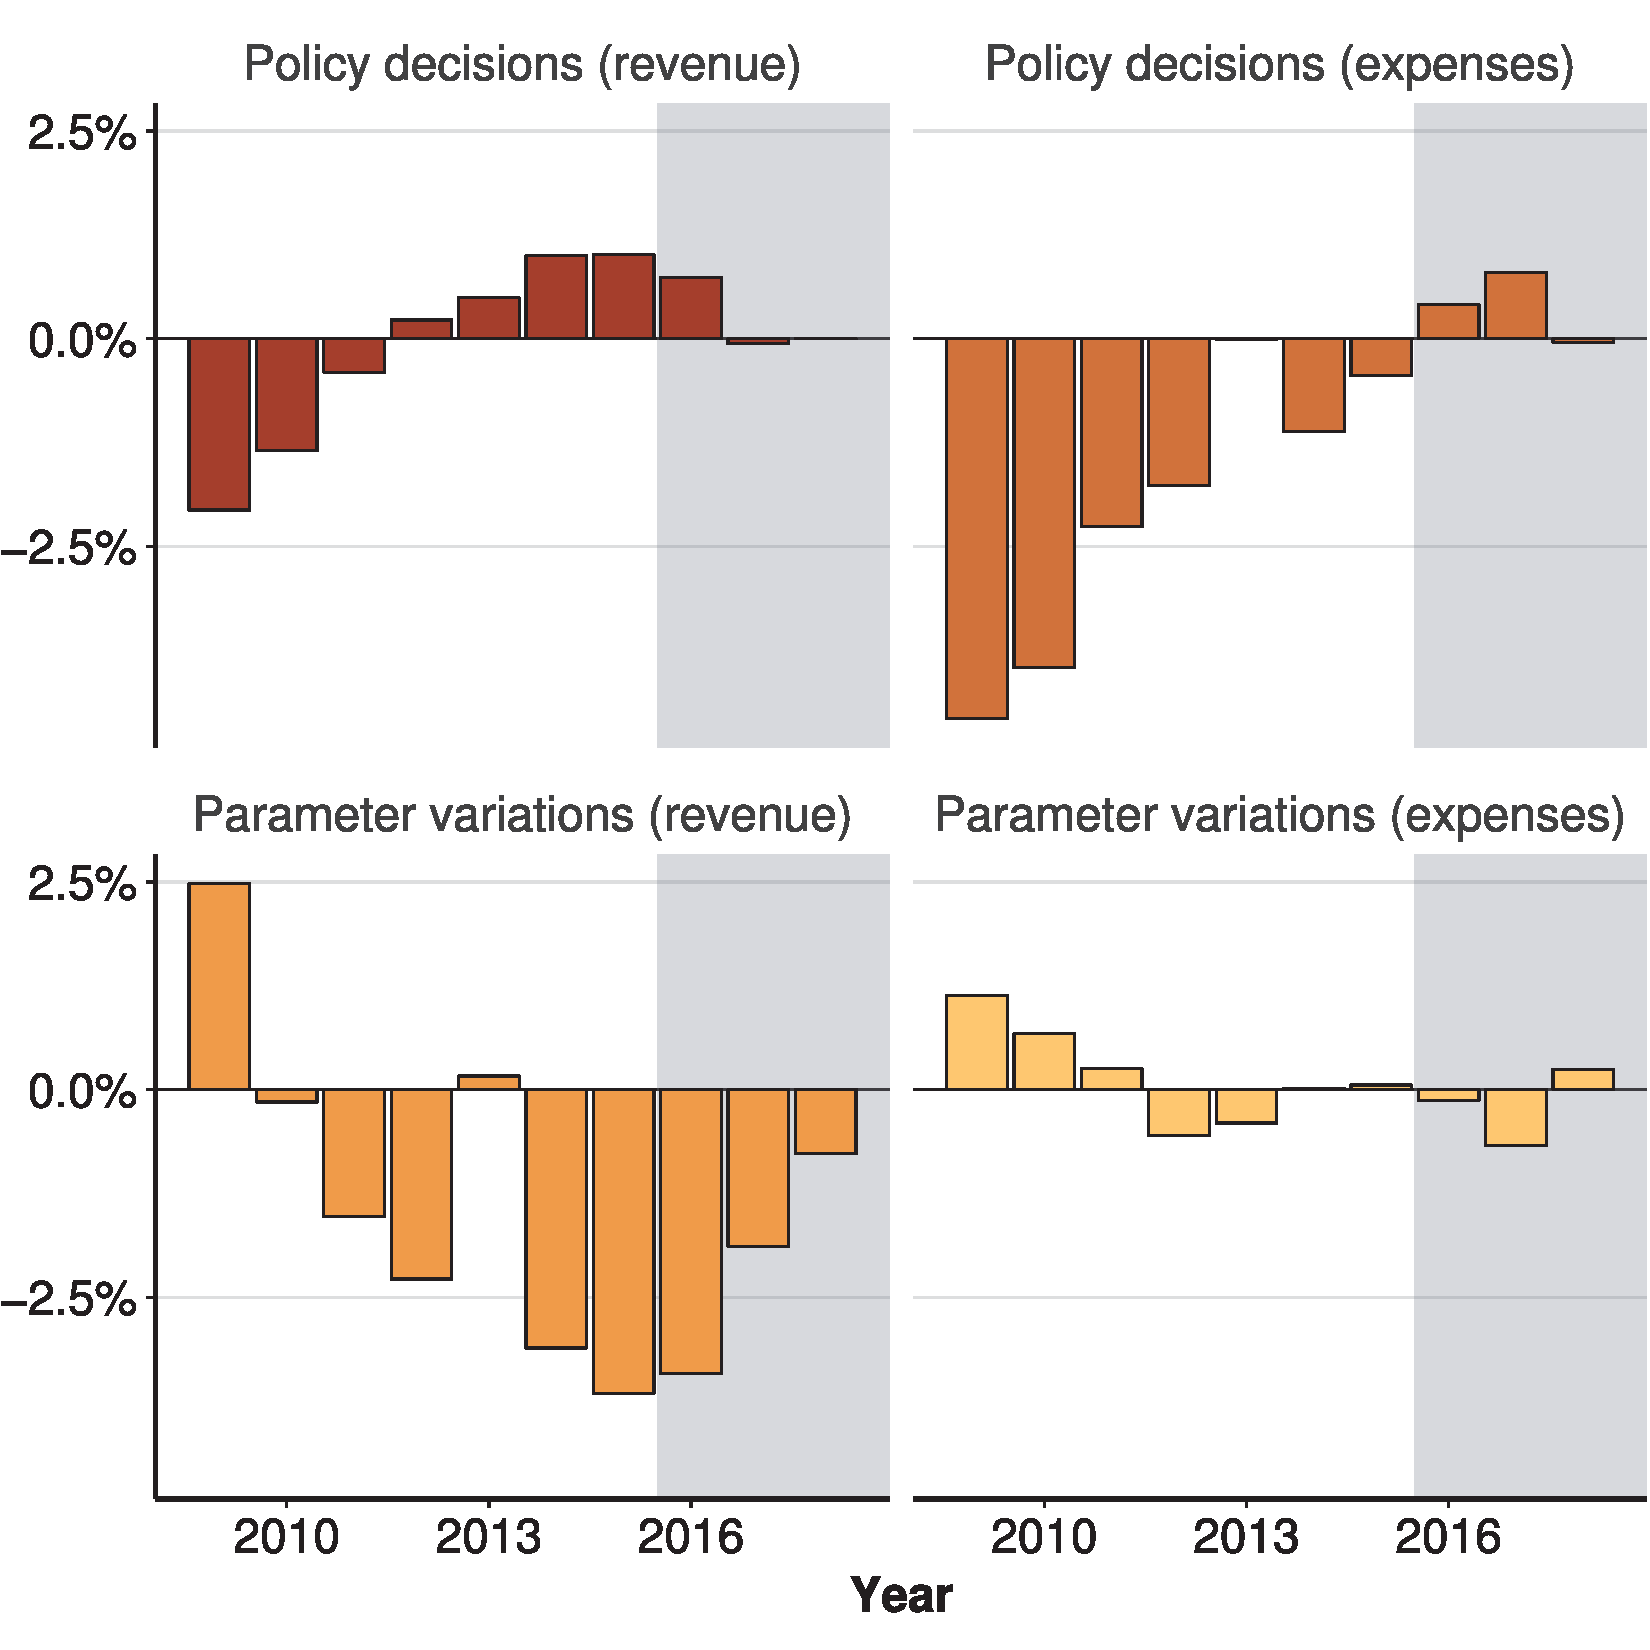
\includegraphics[width=\linewidth]{Fiscal-challenges/figure/Figure10-wrapped-1.pdf}
\notes{The cumulative change for each year from 2009 to 2015 is the cumulative change over four years from the initial projection to the final outcome. For 2016 to 2018, it is the cumulative change from the initial projection to the latest estimate. Expressed as a percentage of nominal GDP in the outcome year.}

\source{Commonwealth Budget Papers, Mid-year Economic and Fiscal Outlook statements, Pre-Election Economic Outlook and Economic Statements (various years).}
\phantom{.}

\vspace{0.10\textheight}\phantom{.}
\end{figure}

But just as the earlier estimates failed to foresee the surge in revenue in the years leading up to the GFC, later estimates have failed to capture its decline. For the last two years, declines in revenue parameter estimates, particularly the terms of trade, have reduced budget balances from the original projections by more than 3~per~cent of GDP\@. Policy decisions have not helped – new spending policies were not always matched by new revenue measures so budget positions deteriorated further from the projections in most years. 

The scale of these errors – larger than the ultimate deficit in most years – calls into question a do-nothing budget strategy that justifies deficits on the basis of a projected surplus or near surplus at the end of the forward estimates period. 

\begin{smallbox}{Electoral sweeteners -- a recent history}{box:FISCAL-1}
Governments of both persuasions like to promise to lift welfare payments, cut taxes and improve government services, especially in election years.  

In the last decade, Age Pension recipients have been the greatest beneficiaries of discretionary top ups. Increases in pension payments over and above the normal indexation arrangements were made in 2007 in the Simpler Superannuation changes, in the 2008\nobreakdash-09 and 2009\nobreakdash-10 Budgets, and in late 2011 as part of the carbon pricing compensation package.  

Recipients of Family Tax Benefit Part B, the Disability Support Pension, Carer Income Support and childcare payments also received one or more discretionary increases 

In 2009-10 higher education received a significant funding boost for teaching and research and reforms to the student income support system. In primary health, funding was boosted by the Bulk Billing Incentive and Extended Medicare Safety Net in 2004, by increasing GP benefits payments in 2005 and by the inclusion of dental services in 2007. 

\boxsources{\textcite{PBO2014}; Commonwealth Budget Papers 2002-03 to 2012-13.}
\end{smallbox}

\@openrighttrue\makeatother

\chapter{State government budgets also face growing pressures\label{chapter:FISCAL-4}}
In contrast to the Commonwealth, state government operating revenues have generally exceeded expenses over the last decade (\Vref{fig:FISCAL-11}). Yet states spent more over the last six years than over the previous six. State revenues and spending are both forecast to fall over the forward estimates. 

\begin{figure}[p]
\captionwithunits{State government budgets have been largely in balance\label{fig:FISCAL-11}}%
{Per cent of nominal GDP}
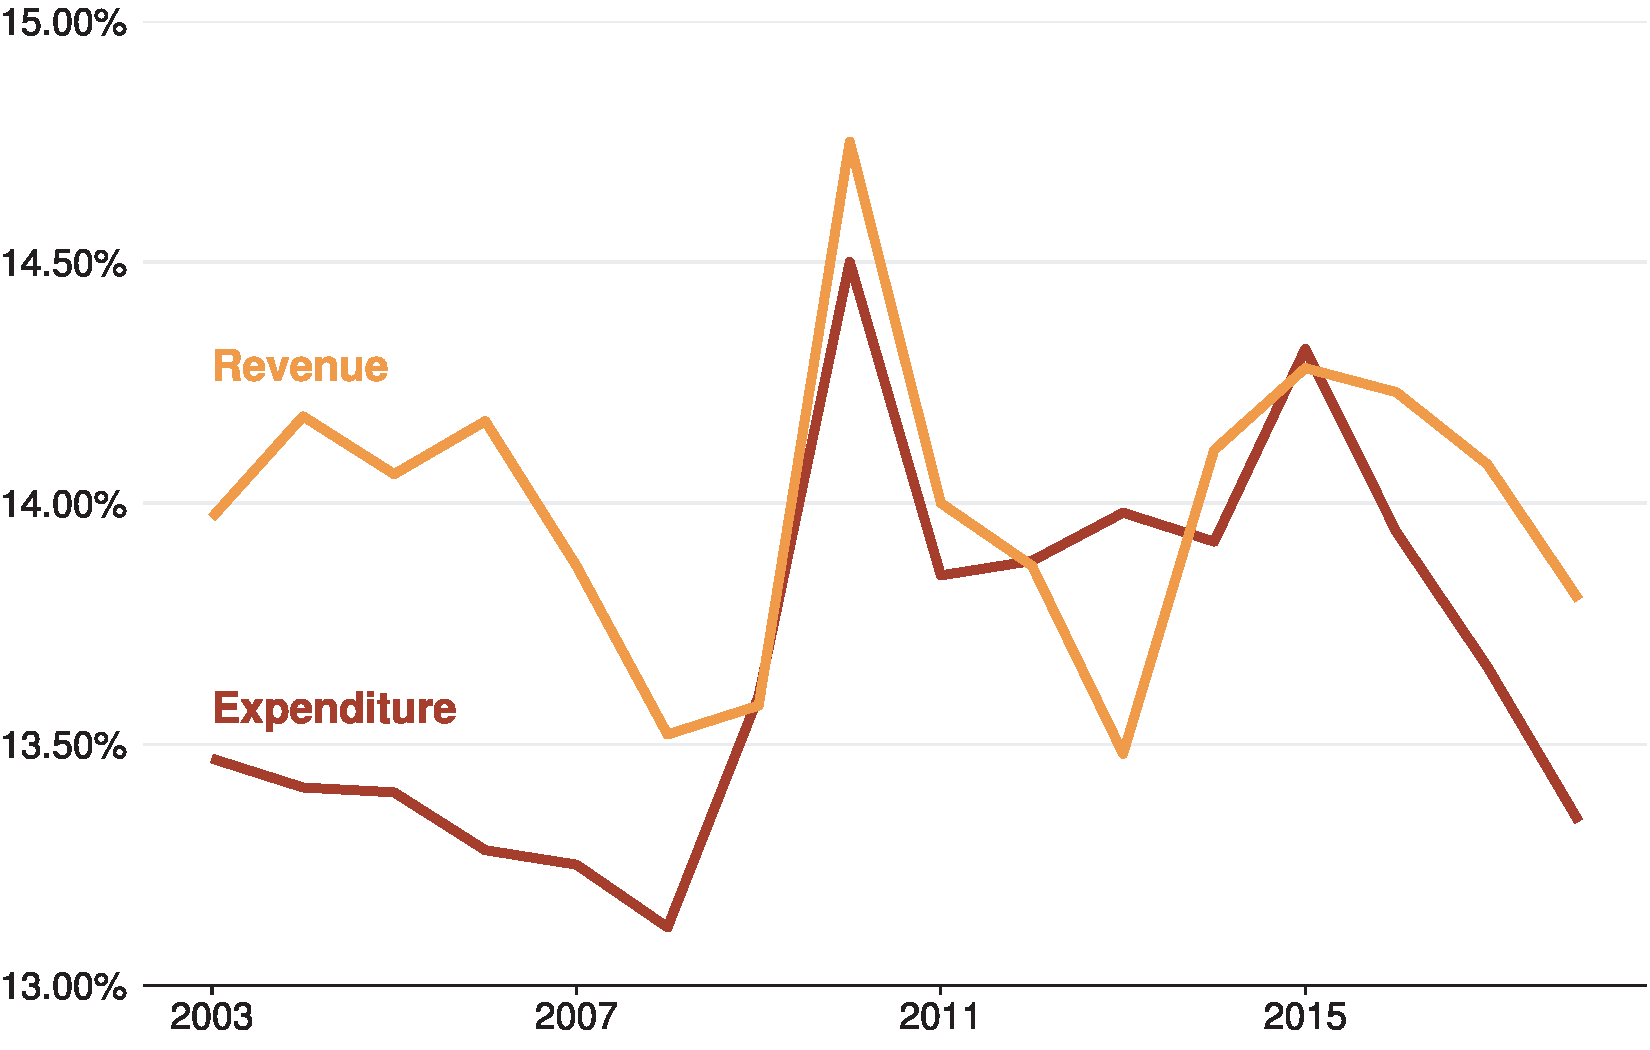
\includegraphics[width=\columnwidth]{Fiscal-challenges/figure/Figure11-1.pdf}
\fnotes{fig:FISCAL-11}{The 2014-15 Budget Papers for many state governments were released prior to the Commonwealth Government budget so forecasts do not include the full impact of reduced Commonwealth funding for health previously agreed under the National Health Reform Agreement. This equates to around \$1.2 billion in revenue (0.06\% of GDP) in 2017-18. }

\source{\textcites{Treasury2014-MYEFO-2014-15}[][Table~1]{ABS2014c}; Grattan analysis.}
\end{figure}

These aggregates obscure variations between states. Tasmania and South Australia ran operating deficits after property market turnover declined and stamp duty revenues fell in 2010-11. Their budget positions have since improved. In Queensland, deficits were larger when revenues were hit by the 2011 floods, but the return to surplus was faster. The NSW, Victoria and Western Australia Government operating budgets were largely balanced over the period. More recently, Western Australia went into deficit when royalty revenues from iron ore fell sharply. This was exacerbated by the fall in their share of GST revenues as the Grants Commission process redistributed record state mining royalty revenues from previous years which had already been spent by the WA Government.

Unlike the Commonwealth, the states also have significant capital spending that does not immediately affect net operating balances.\footnote{The depreciation on this capital spending affects net operating balances in subsequent budget years. Non-cash depreciation already built into state operating budgets will erode this debt if state capital spending falls, as their most recent budgets forecast.}  Capital spending increased substantially after 2005, and far exceeded the offsetting depreciation of previous capital spending. State governments funded this increased infrastructure spending largely through borrowing, and so net debt increased (\Vref{fig:FISCAL-12}). In the decade to 2013-14, higher interest and depreciation costs increased subsequent operating budget expenses from six to more than nine per cent of state revenues.\footcite[][41]{DaleyWoodWeidmannEtAl2014}

\begin{figure}[p]
\captionwithunits{State and territory net debt increased rapidly\label{fig:FISCAL-12}}%
{Total state and territory net operating balances and debt, (2014 dollars)}
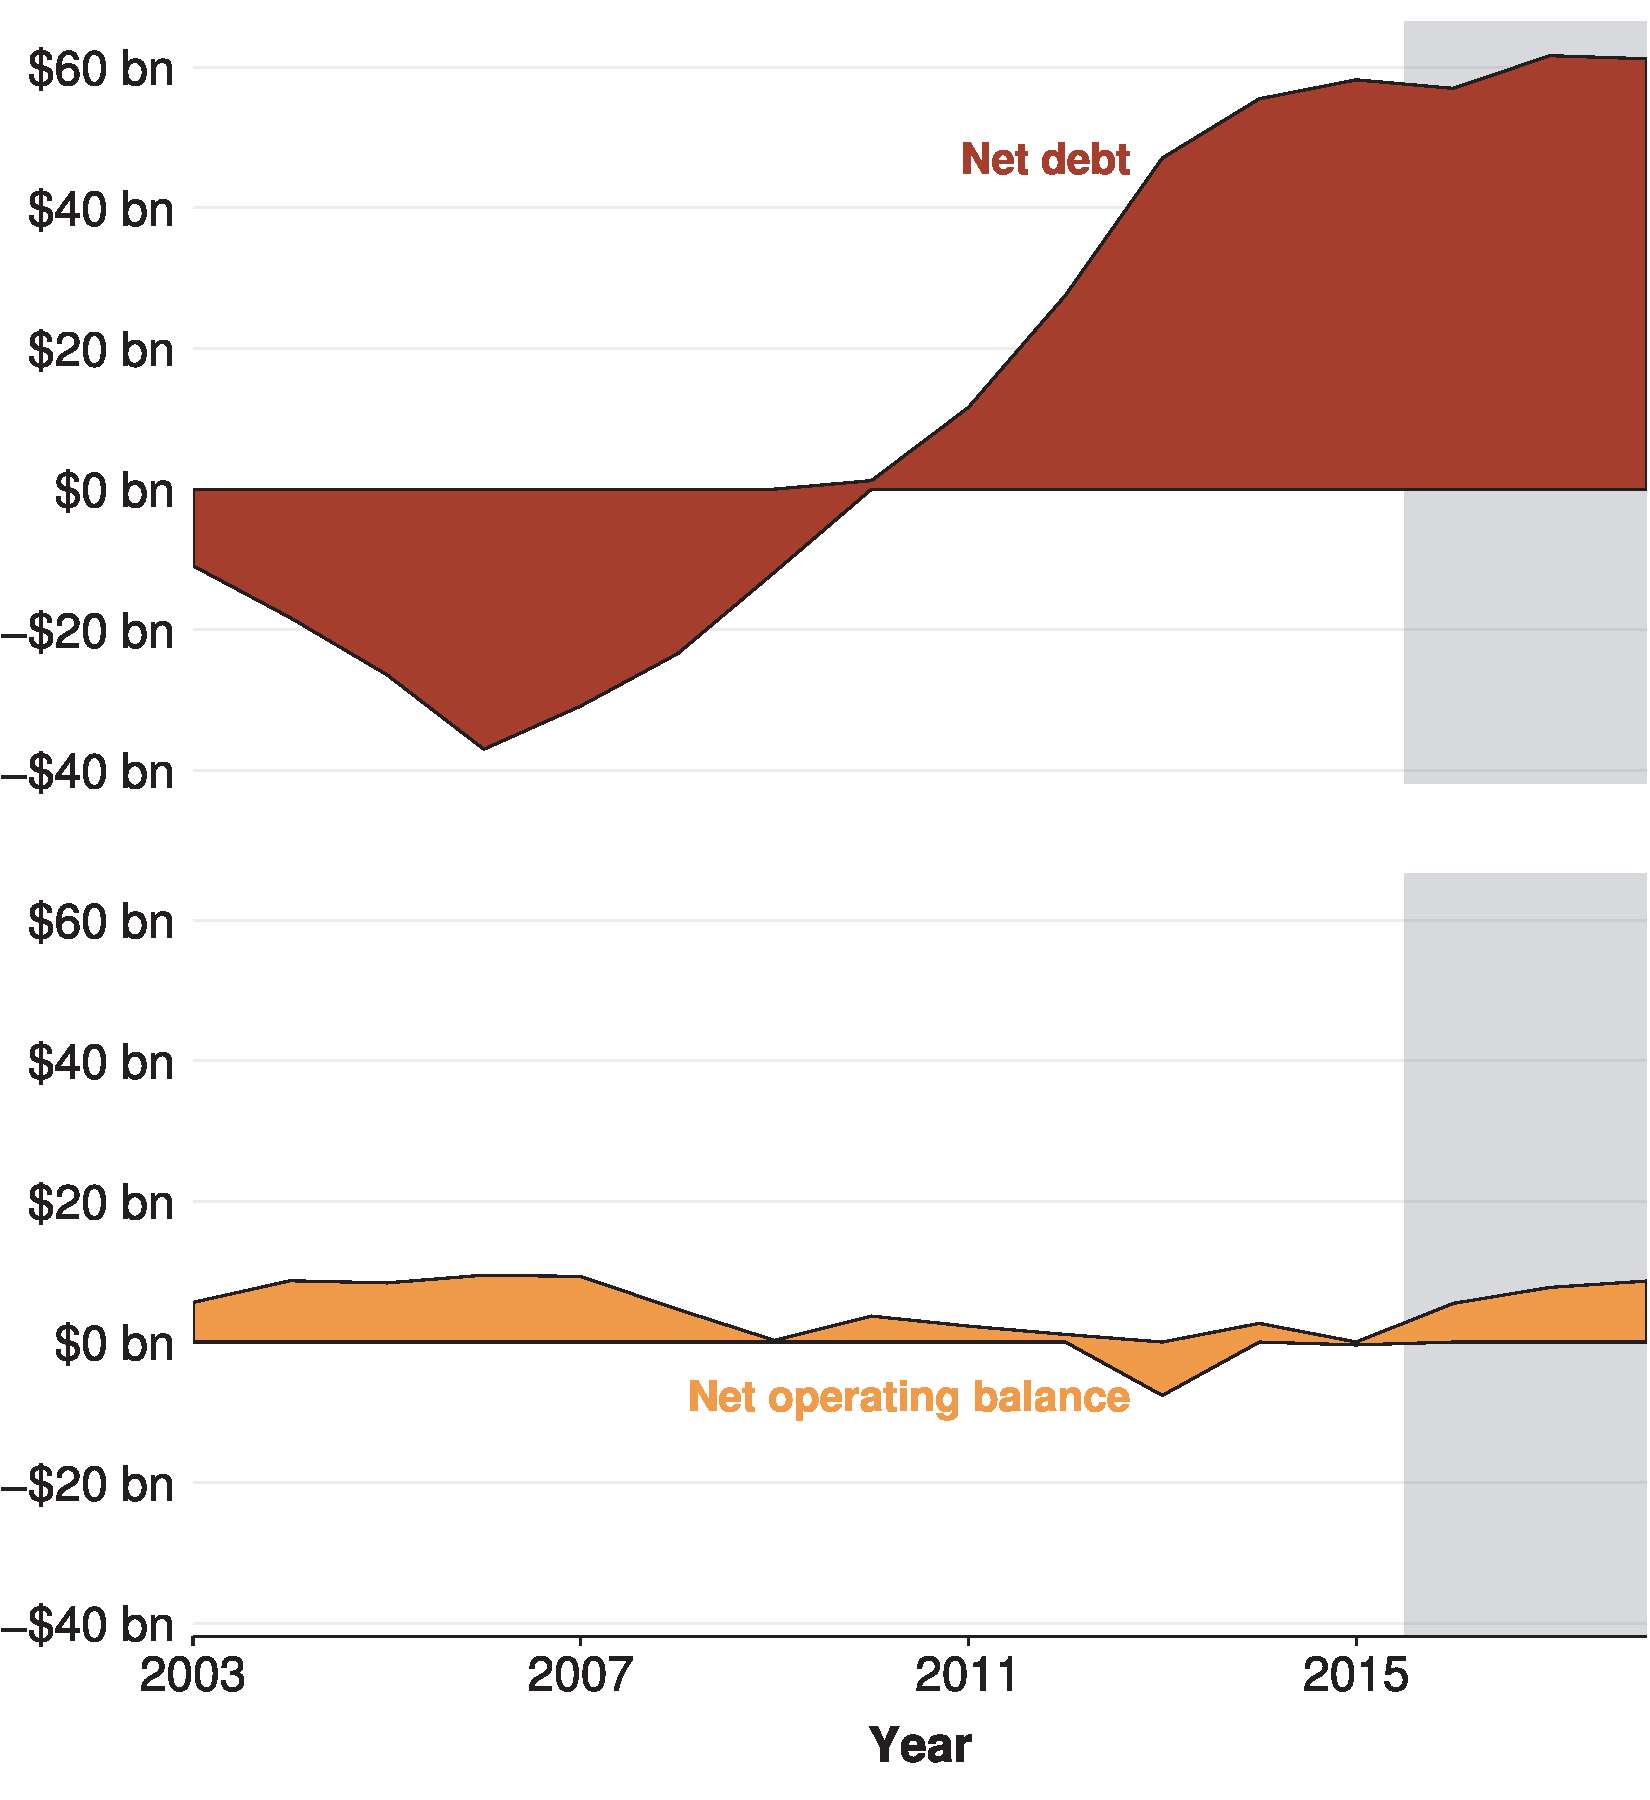
\includegraphics[width=\columnwidth]{Fiscal-challenges/figure/Figure12-1.pdf}
\fnotes{fig:FISCAL-12}{Debt forecasts in NSW, Queensland, South Australia and ACT were revised downwards between the 2013-14 Budget and the 2014-15 Budgets and Mid-Year forecasts. This accounts for the lower combined debt forecasts compared to those presented in our 2014 Budget Pressures report \textcite[][41]{DaleyMcGannonHunter2014}.The improvement in the forecast debt position was particularly significant in NSW because of the sale of Macquarie Generation in September 2014.}

\source{State government Budget Papers and Mid-Year forecasts.}
\end{figure} 

\FloatBarrier

\section{Future pressures on state government budgets\label{sec:FISCAL-4-1}}
All state governments will face more significant budget pressures beyond the forward estimates. Health and education spending are forecast to grow strongly over the next decade. At the same time, the Commonwealth has stated that from 2017-18 it will no longer contribute to growth in real spending per person in these areas. Health and education make up almost half of state government expenditure. If spending per person continues to grow faster than inflation, then it is unlikely that other areas can be cut enough to make up the gap. Instead, state governments will need additional revenues to keep their budgets balanced.

\section{More spending on hospital, schools, and infrastructure\label{sec:FISCAL-4-2}}
Growing healthcare costs are the most significant spending pressure on state governments. Spending on health, primarily hospitals, is about 25~per cent of state recurrent expenditure.\footcite[][4]{DaleyMcGannonHunter2014}

State government health spending grew considerably faster than the economy over the last two decades. Increased use of services rather than population ageing was the main cause of health spending growth (\Vref{fig:FISCAL-13}).\footcite[][26]{DaleyWoodWeidmannEtAl2014}  As the economy grew, governments spent more of their income providing more and better health treatments, including those using new technologies.\footcite{gruen2007conceptual}

\begin{figure}
\captionwithunits{All age groups contributed to increased health spending\label{fig:FISCAL-13}}%
{Increase in real government health spending, 1989 to 2010}
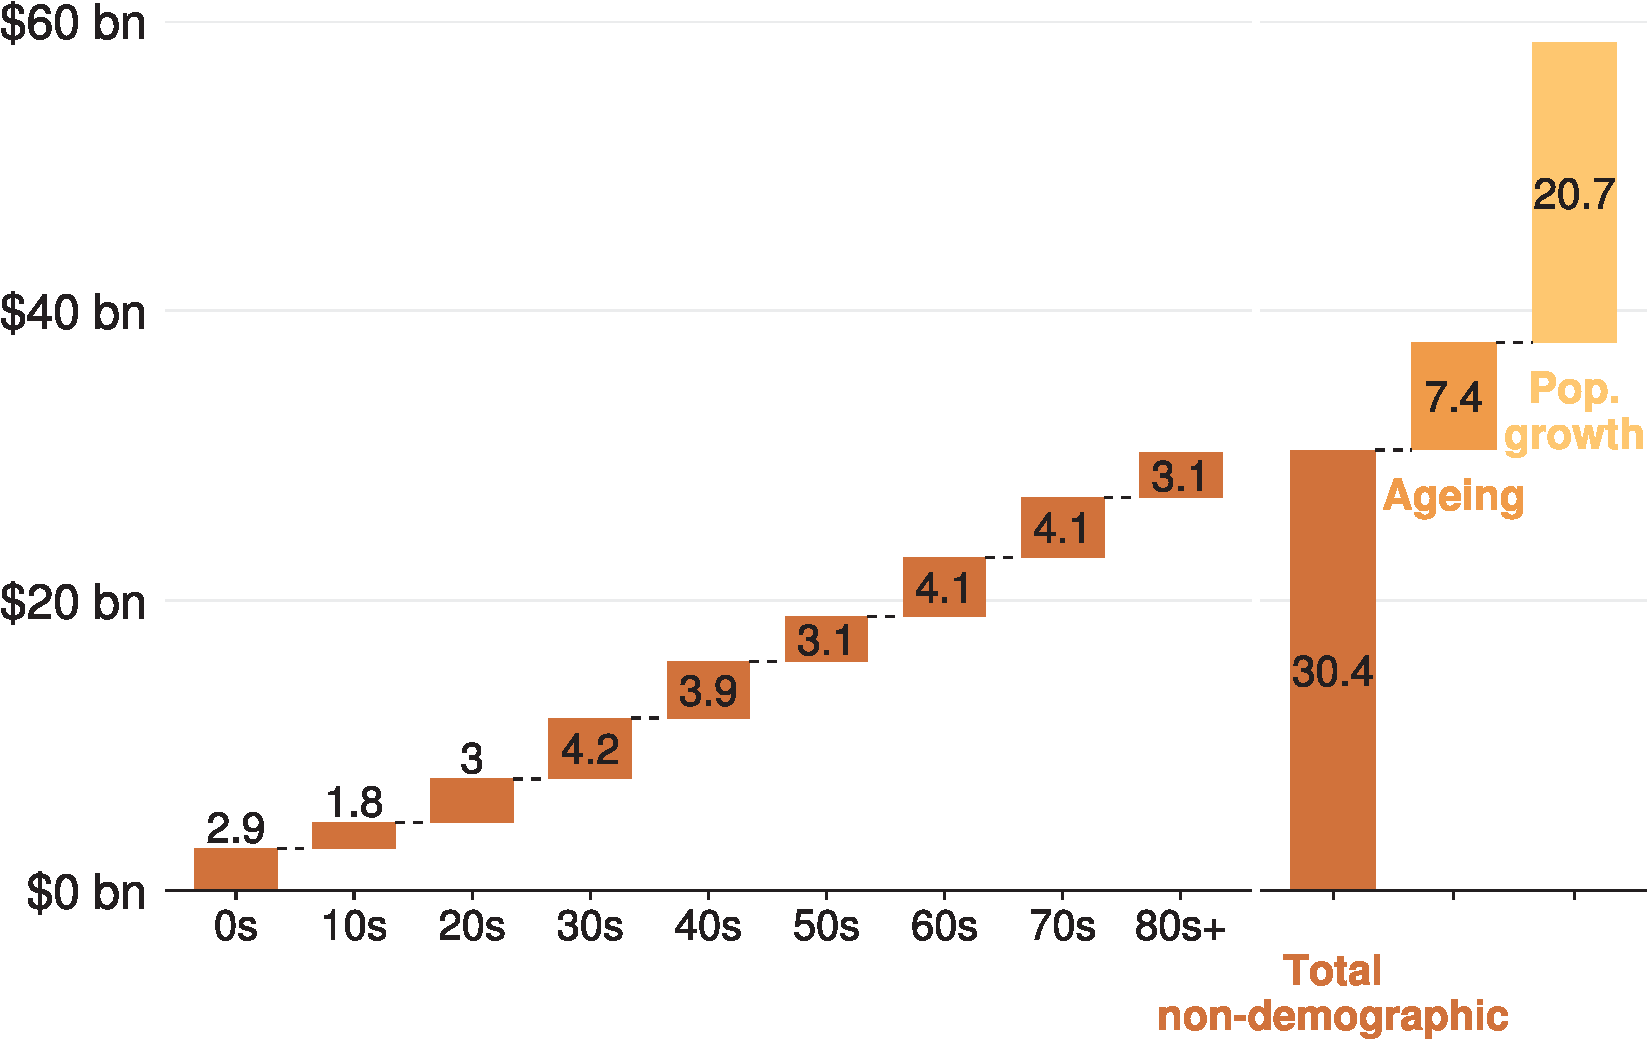
\includegraphics[width=\columnwidth]{Fiscal-challenges/figure/Figure13-1.pdf}
\fnotes{fig:FISCAL-13}{Less reliance ought to be placed on figures for 80+, as sample sizes are small and data categories change across surveys. Spending figures are adjusted to constant prices using the GDP implicit price deflator. Since health prices grew somewhat faster than average price levels, a small proportion of the increase across all categories will reflect this faster price growth.}

\source{\textcites{ABSVariousyearsc}[][Table~59]{ABS2014d}; Grattan analysis.}
\end{figure}

This strong non-demographic growth is forecast to continue.\footcite{ProductivityCommission2013AgeingAustralia}  Population ageing will also contribute more to spending growth as the large baby boomer cohort reaches the age brackets when health spending per person is much higher.\footcite[][26]{DaleyWoodWeidmannEtAl2014}  

State government spending on schools is also forecast to rise faster than GDP in years to come. The increase is partly a result of commitments to increase funding for schools with disadvantaged students between 2014 and 2019 under the National Education Reform Agreement.  

State governments spent more on infrastructure – particularly in transport – over the last decade (\Vref{fig:FISCAL-14}).\footnote{These estimates based on engineering work done are consistent with ABS statistics based on government budget papers \textcite[][41]{PBO2015a}.}  Much of it was effectively unfunded. Although state spending on infrastructure is now falling, there will be significant pressure to maintain or increase spending on infrastructure to cope with increasing population and concerns about congestion.\footcites[][112-128]{KellyDonegan2015}{InfrastructureAustralia2015-InfrastructureAudit}

\begin{figure}
\captionsetup{oneside, margin={0cm,-2cm}}
\captionwithunits{Government infrastructure spending rose from 2007, but is now falling\label{fig:FISCAL-14}}%
{Engineering construction work done for the public sector, \%\ of GDP}
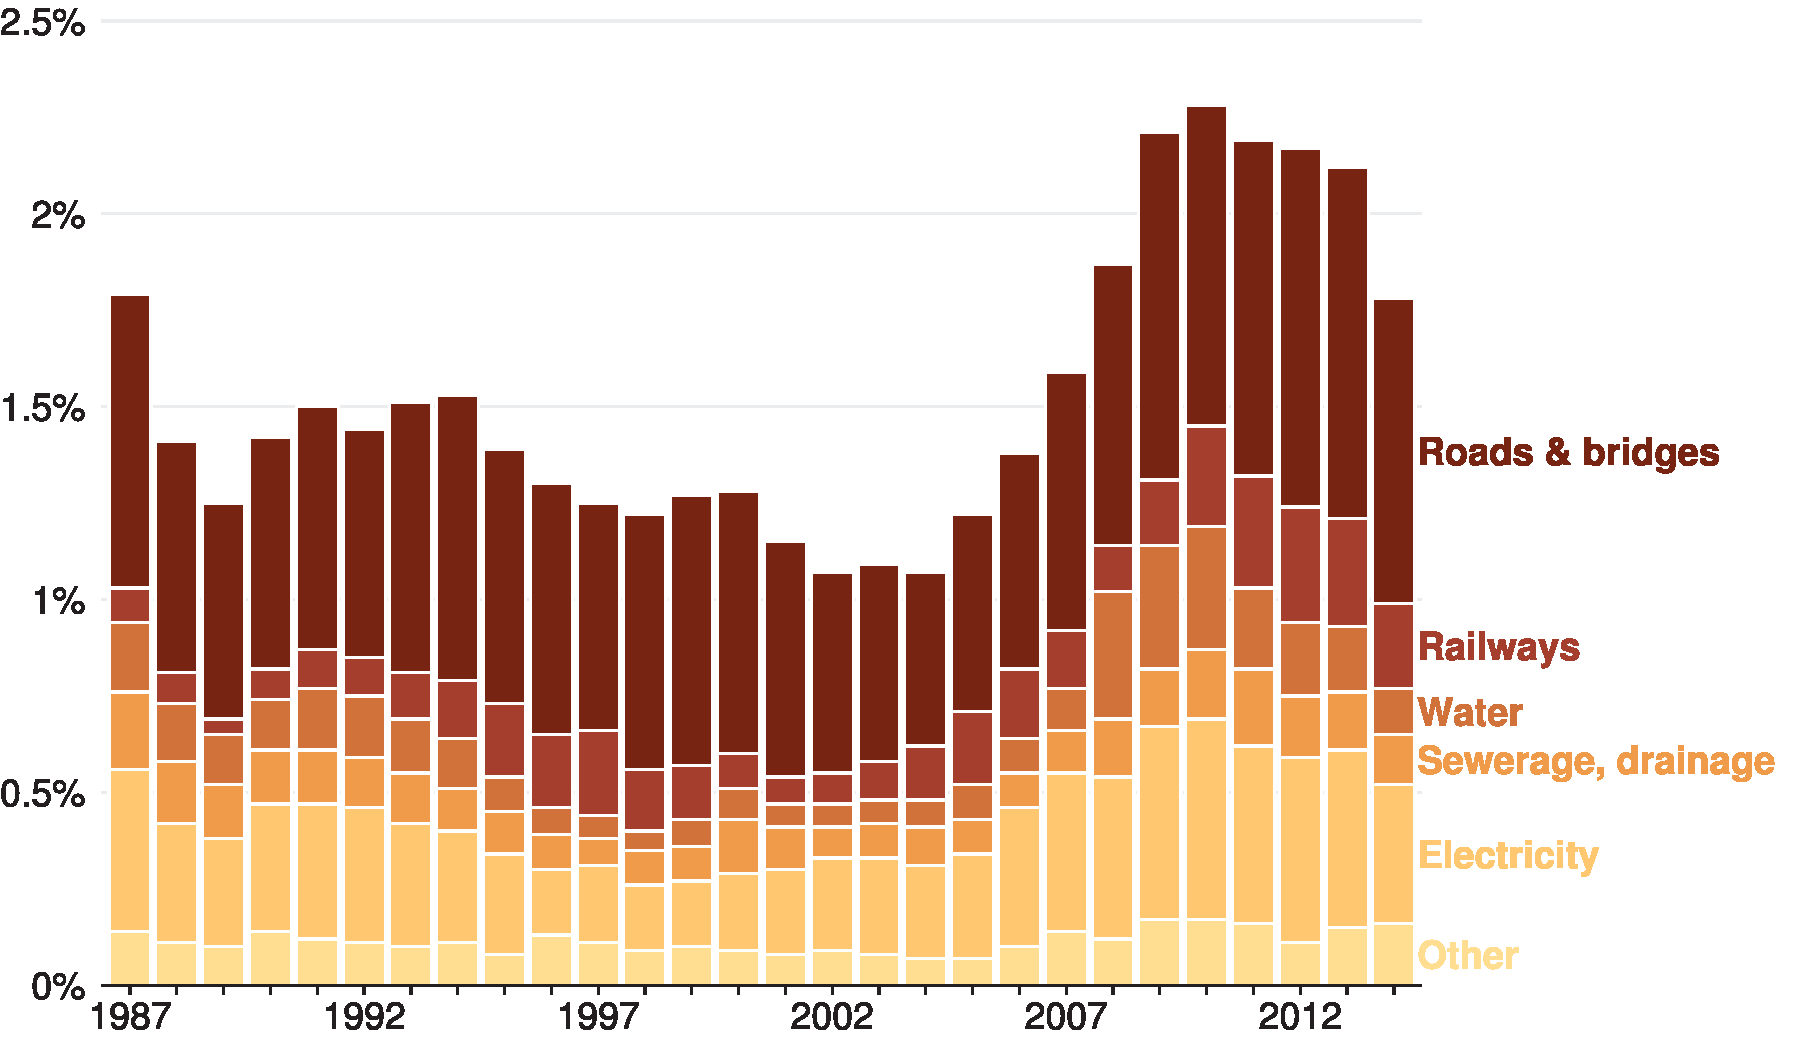
\includegraphics[width=1.1\columnwidth]{Fiscal-challenges/figure/Figure14-1.pdf}
\notes{By financial year. Excludes telecommunications, insignificant after Telstra sale.}

\source{\textcite{ABS2015b}}
\end{figure}

Higher infrastructure spending can be justified if it generates increases in the productive capacity of the economy sufficient to justify the cost. But Australian governments could do a lot better in their project choices. An overhaul of project selection processes – including greater reliance on independent and transparent cost-benefit analysis – would significantly improve the returns to this spending.\footcite{ProductivityCommission2013PublicInfrastructure} 

\section{The Commonwealth has substantially reduced planned funding for the states\label{sec:FISCAL-4-3}}
Under Commonwealth policy adopted in the May 2015 budget, state governments will have to fund all increases in real spending per person for hospital and schools.\footcite[][BP~No.~2, p.~126]{Treasury2014-Budget-Papers-2014-15}  The change abandoned previous Commonwealth undertakings, set out in the COAG National Education Reform Agreement and the National Health Reform Agreement, to contribute to real increases in spending per person.

The shift in spending responsibility back to the states is very significant. The Commonwealth estimates that by 2024-25 the changed policy will reduce its real spending by \$11 billion on hospitals and \$5~billion on schools.\footnote{Estimates in 2013-14 dollars. Schools estimate calculated from nominal value of transfer provided in \textcite[][Overview, p.~7]{Treasury2014-Budget-Papers-2014-15}. Health estimates based on \textcite{Hockey2015IGR}.}  By 2054-55, the reduction in real spending for hospitals could be as large as \$78 billion (\Vref{fig:FISCAL-15}).  

\section{Other State revenues are also under pressure\label{sec:FISCAL-4-4}}
State revenues may also come under renewed pressure. Relatively constant revenues over the last decade may have masked increased vulnerabilities in individual revenue sources.

In particular, untied revenues from the GST fell over the decade, from almost 4.0~per~cent to 3.2~per~cent of GDP in the decade to 2013-14. The main causes were people saving more and spending more on untaxed goods and services, particularly rent and mortgage payments.\footcite[][34]{DaleyWoodWeidmannEtAl2014}  Unless these trends reverse, GST is unlikely to increase as a percentage of GDP.

Conveyance stamp duties also fell. They averaged about 1.2~per~cent of GDP between 2002-03 and 2007-08, but only 0.9~per~cent of GDP since then.\footcite{PBO2015a} 

These falls over the decade were offset by rises in royalties and small increases in property and payroll taxes. Yet state royalties are now falling as price falls outweigh volume increases.\footnote{State royalties are typically value-based; they are not simply charges based on volume.}  All states effectively benefited from the rise in royalties, and will feel the pinch if they fall. Revenue redistribution determined by the Commonwealth Grants Commission and implemented through the carve up of the GST means that changes in one state’s royalties are effectively shared among all states.

\begin{figure}[hbp]
\captionwithunits{Commonwealth will provide much less funding to the states for health than previously agreed\label{fig:FISCAL-15}}%
{Forecast Commonwealth health funding withdrawn from states (2014 dollars)}
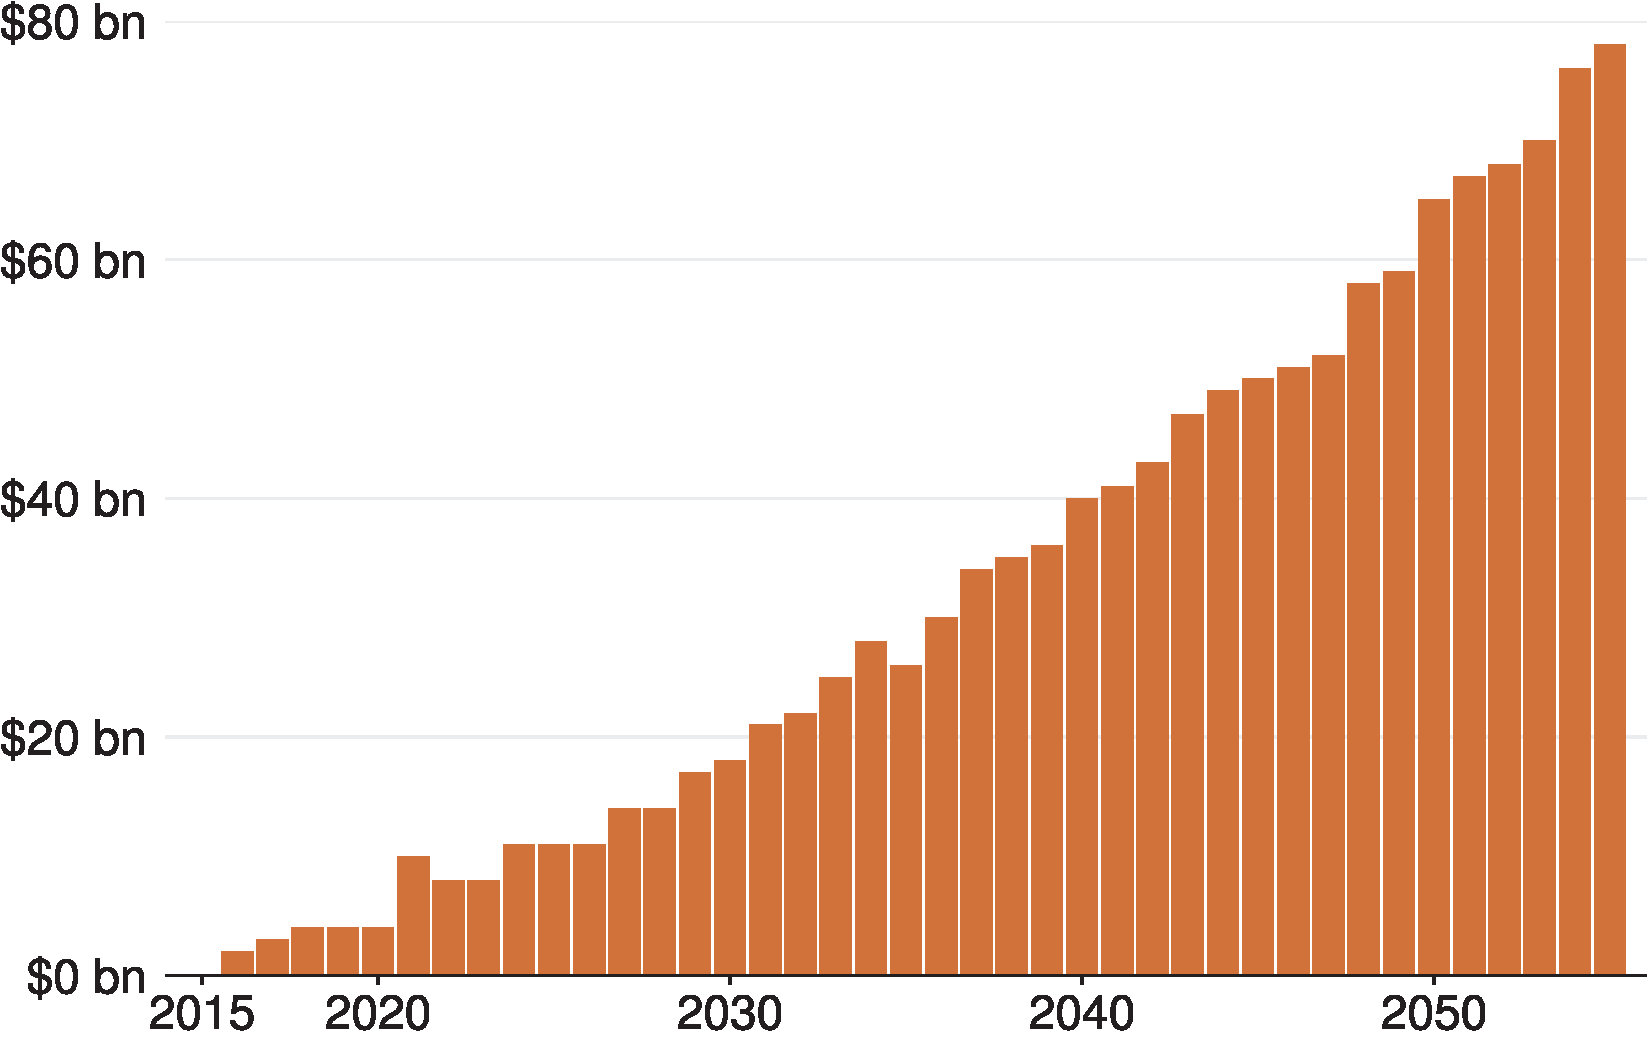
\includegraphics[width=\columnwidth]{Fiscal-challenges/figure/Figure15-1.pdf}
\notes{Estimates of health funding withdrawn from states based on the difference in Australian Government spending under the `proposed policy' and `previous policy' scenarios modelled in \textcite[][Tables~2.10 and C.2]{Hockey2015IGR}.}
\end{figure}

\chapter{What should governments do?}
Australian governments are running substantial budget deficits. Future pressures are likely to make the problems worse. A drift back to surplus is unlikely, and relies on best case assumptions that have often disappointed in the past. 

There have been a range of justifications for inaction. Governments have taken advantage of the wriggle room provided by the vagueness of where Australia is in the economic cycle. For several years they have played St Augustine: “let us be chaste and run a surplus – but not yet.” And while they have pointed to sluggish economic growth to justify deficits, they have glossed over the temporary boost to revenues from the mining boom. Finally, they have talked up their position by pointing to surpluses or near surpluses towards the end of each budget’s forward estimates. These mirages\DEVIATION{} have continued to recede to the horizon as optimistic projections have run aground on reality.

To bring their budgets back to balance, governments will need to undertake reforms on both the revenue and the spending side. But recently the Commonwealth Government’s energy has been focussed on cuts to spending. There have been large reductions in the budget for foreign aid%
\footnote{The 2014-15 Budget cut proposed spending for official development assistance (ODA) by \$7.6 billion over five years (\textcite[][121]{Treasury2014-Budget-Papers-2014-15}). Another \$3.7 billion in savings over four years was announced in MYEFO 2014-15 (\textcite[][47]{Treasury2014-MYEFO-2014-15}).} %  
and sizeable savings have also been proposed (and in some cases reversed) for higher education, primary care, and welfare through changes in eligibility thresholds and indexation arrangement for benefits.\footcites[][BP~No.~2, pp.~7,~133, 197--204, 210]{Treasury2014-Budget-Papers-2014-15}  The Commonwealth Government has deferred any significant changes in its revenue mix until after its \emph{Tax White Paper}.\footcite{Loughnane2013} 

Most state governments have also shown a lack of enthusiasm for new revenue measures.\footnote{Very few state governments have engaged in serious debate about tax reform in recent years. Indeed, the trend in election campaigns has been to rule out any changes to taxation. In the recent Victorian election campaign, the Labor Opposition committed to no new taxes or tax increases if they won power (\textcite{Savage2014}). The LNP made similar commitments in the Queensland Election campaign (\textcite{Eaton2015}). One exception is South Australia that has recently released a comprehensive discussion paper on State Tax Reform (\textcite{GovernmentSouthAustralia2015-State-Tax-Review-Discussion-Paper}).}  These governments, after benefiting from high mining royalty revenues, have offered no plan to fill the gap as these volatile revenues wane. 

But there are revenue measures that could make a meaningful contribution to budget repair with little collateral damage. In the following parts, we set out four policy proposals – reducing superannuation tax concessions, changes to capital gains tax and negative gearing, broadening the GST and the introduction of a broad-based property levy – that we think governments should adopt to improve their fiscal position.

These reforms will be politically difficult. To build the public case, governments should adopt budget projection methodologies that provide a more realistic picture of the pressures on Australia’s medium term budget outcomes. These will make it more obvious that we cannot rely on the hope that our luck will improve. Tougher decisions are needed. 

% \flushcolsend

\part{Property taxes}\label{part:PROP}
\makeatletter\@openrightfalse\makeatother
\cleardoubleevenstandardpage
\begin{overviewNoClearPage}[-25pt]
The previous part, \textit{Fiscal Challenges for Australia}, originally published in July 2015,\DEVIATION{} shows how Commonwealth and state government budgets are under pressure. The Commonwealth Government has run deficits for six years, largely because its spending on older households has increased rapidly. 

State government spending on health and education and other vital areas is also growing faster than GDP\@. State revenues are threatened by the Commonwealth’s decision in the 2014-15 Budget to ease some of its own budget pressures by substantially reducing promised funding to the states for hospitals and schools. Recent state government budgets provide no insight into how they will respond to the looming funding gap. 

This part shows how a broad-based property levy could help repair state government revenues without damaging the economy or the most vulnerable in our society.

Property taxes – which are levied on the value of property holdings – are the most efficient taxes available to the states. If they are designed well and applied broadly, property taxes do little to change incentives to work, save and invest. Unlike capital, property is immobile – it cannot shift offshore to avoid higher taxes. Concerns about the risks of multinational tax avoidance, the increasing mobility of capital around the world, and the increasing value of residential property relative to incomes, should make property taxes a priority in any tax reform.

The property tax base is large and growing fast. A low-rate, broad based property levy using the council rates base could raise about \textbf{\$7~billion} a year for state and territory governments through an annual levy of just \$2 for every \$1000 of unimproved land value, or \$1 for every \$1000 of capital improved property value. 

The costs to property owners would be manageable. A home-owner would pay a levy of \$772 a year on the median-priced Sydney home, valued at \$772,000, or \$560 a year on the median-priced Melbourne home valued at \$560,000. People with low incomes and no wealth would pay nothing. Low-income retirees with high value houses could defer paying the levy until their house is sold.

Higher property taxes could also be used to fund the reduction and eventual abolition of state stamp duties on property. Stamp duties are among the most inefficient and inequitable taxes available to states, and their revenues are inherently volatile. Although abolishing stamp duties is not the focus of this report, shifting from stamp duty to a broad-based property tax would provide a more stable tax base for states, spread the tax burden more fairly, and add up to \$9 billion annually to GDP. 

Calls to reform property taxes are not new. Property taxes are often unpopular precisely because they are highly visible and difficult to avoid. Yet they are also efficient and fair, and don’t distort behaviour. Greater use of property taxes would be the best way for state governments to meet the growing pressures on their budgets.
\end{overviewNoClearPage}
\makeatletter\@openrightfalse\makeatother
\chapter{State government budgets face growing pressures}\label{chapter:PROP-1}
The Commonwealth is not the only government under significant budgetary pressure. The previous part shows that all state governments face growing budget pressures beyond the four-year forward estimates. 

State government spending on health and education and other vital areas is growing faster than GDP\@. Most states significantly increased infrastructure spending over the last few years, and largely funded this through borrowing, so that future budgets must spend more to service the debt and depreciation. 

Other pressures are threatening state revenues. Relatively constant revenues over the last decade may have masked increased vulnerabilities in individual revenue sources. In particular, untied revenues from the GST fell over the decade.\FOOTNOTE{See \Vref{sec:FISCAL-4-4}.}  These falls were offset by rises in mining royalties and small increases in property and payroll taxes. Yet state royalties are now falling as commodity price falls outweigh volume increases.\footnote{State royalties are typically value-based; they are not simply charges based on volume.}  As a result of GST distributions, all states effectively benefited from the rise in royalties, and all will suffer if they fall. 

State revenues are also threatened because of planned reductions in grants from the Commonwealth for schools and hospitals.  The Commonwealth’s decision to no longer contribute to growth in real spending per person in these areas beyond 2017-18 presents the states with a potential \$16~billion revenue shortfall by 2024-25, and a big problem.\FOOTNOTE{See \Vref{sec:FISCAL-4-3}.}  If spending per person continues to grow faster than inflation, then it is unlikely that other areas can be cut enough to make up the difference. 

Recent budgets provide no insight into how state governments will respond to the looming funding gap. Most have shown a lack of enthusiasm for new revenue measures or substantive tax reforms.\footnote{While South Australia has announced the abolition of stamp duties on commercial property following the release of a comprehensive discussion paper on State Tax Reform (\textcite{DTF2015-State-Budget-Papers-201516}), it hopes to fund this largely through an increased share of GST revenues (\textcite{GovernmentSouthAustralia2015-State-Tax-Review-Discussion-Paper}).}  

Hoping for the best is not a budget management strategy: it simply shifts the costs and risk of budget repair onto future generations. More active policy measures to achieve budget repair are required. While containing spending will be important, both the politics of budget repair and the sheer size of the budget gap mean that governments are unlikely to be able to restore budgets to balance without also boosting revenues.

Sustainable budgets depend on tough choices, not hope. To ensure that future generations do not have to foot the bill for today’s inaction, these choices must be made.


\makeatletter\@openrightfalse\makeatother
\chapter{Property tax reform should be the states' priority}\label{chapter:PROP-2}
Greater use of property taxes is the best way for the states to meet their budget challenges. Property taxes – which are levied on the value of property holdings – are the most efficient taxes available to the states. If they are designed well and applied broadly, they do little to change incentives to work, save and invest.

The property tax base is large and growing fast. A low rate broad property levy using the council rates base could raise about \textbf{\$7~billion a year} for state and territory governments through an annual levy of just \$2 for every \$1000 in unimproved land value, or \$1 for every \$1000 in capital improved values. Although it would have marginally more impact on economic decisions, a levy on capital improved values would still have low economic costs, and may be simpler to implement since capital improved property values are easier to track.

A broad-based property levy might provide a path to longer-term reform of taxation on property, by funding the reduction and eventual abolition of state stamp duties for property. The Commonwealth Treasury nominates stamp duty as Australia’s least efficient tax.\footcite{Treasury2015BudgetPapers201516}  Stamp duties deter people from buying and selling property, and therefore can prevent them moving closer to jobs or upsizing and downsizing homes as their needs change. Stamp duties raised \$16 billion for the states in 2013-14.  Their costs to the economy and jobs are large.\footcite{ABS2015h}

The ACT is phasing out stamp duty over 20 years, and replacing the revenues with higher municipal rates.\footcites[][21]{ACT-Treasury2012-13-Budget-Papers}[][229]{ACT-Treasury2014-15-Budget-Papers}  South Australia plans to abolish stamp duties on commercial property, but has ruled out extending land taxes to owner-occupied housing. The government seems to be relying on higher GST revenues in order to abolish stamp duty, rather than relying more on efficient state taxes.\footcites{GovernmentSouthAustralia2015-Govt-response-to-State-Tax-Review}{DTF2015-State-Budget-Papers-201516} 

Once a broad-based property levy becomes large enough, it might also be possible to phase out land taxes as currently designed. The states raised \$6.4 billion from land taxes in 2013-14, but carve outs from the land tax base (via exemptions for owner-occupied housing), thresholds, and progressive rates make them much less efficient taxes than they should be. 

Property tax reform would also support reforms to the fiscal arrangements of the Australian federation. These reforms are under consideration through the Commonwealth’s 
\citetitle{Abbott2014-White-Paper-Reform-Federation}.
%White Paper on the Reform of the Federation process. 
A broad-based property levy would boost states’ revenues, giving greater control over their own destinies, with minimal drag on their economies. Other options to increase revenues include sharing in Commonwealth income tax receipts, or broadening or increasing the GST\@. Relative to these options, a broad-based property levy would do more to increase state government responsibility for funding their own spending. 

\makeatletter\@openrightfalse\makeatother
\chapter{Property taxes can generate substantial revenues}\label{chapter:PROP-3}
\section{Australian property taxes are relatively low}
Australian governments derive less revenue from property taxes as a share of GDP than they should. Australia’s property tax take is far below that of some comparable countries (\Vref{fig:PROP-1}).

\begin{figure}[!b]
\captionsetup{oneside, margin={0cm,-1cm}}
\captionwithunits{Some countries raise more tax from property than Australia does\label{fig:PROP-1}}%
{Tax revenues from property as a percentage of GDP, 2012}
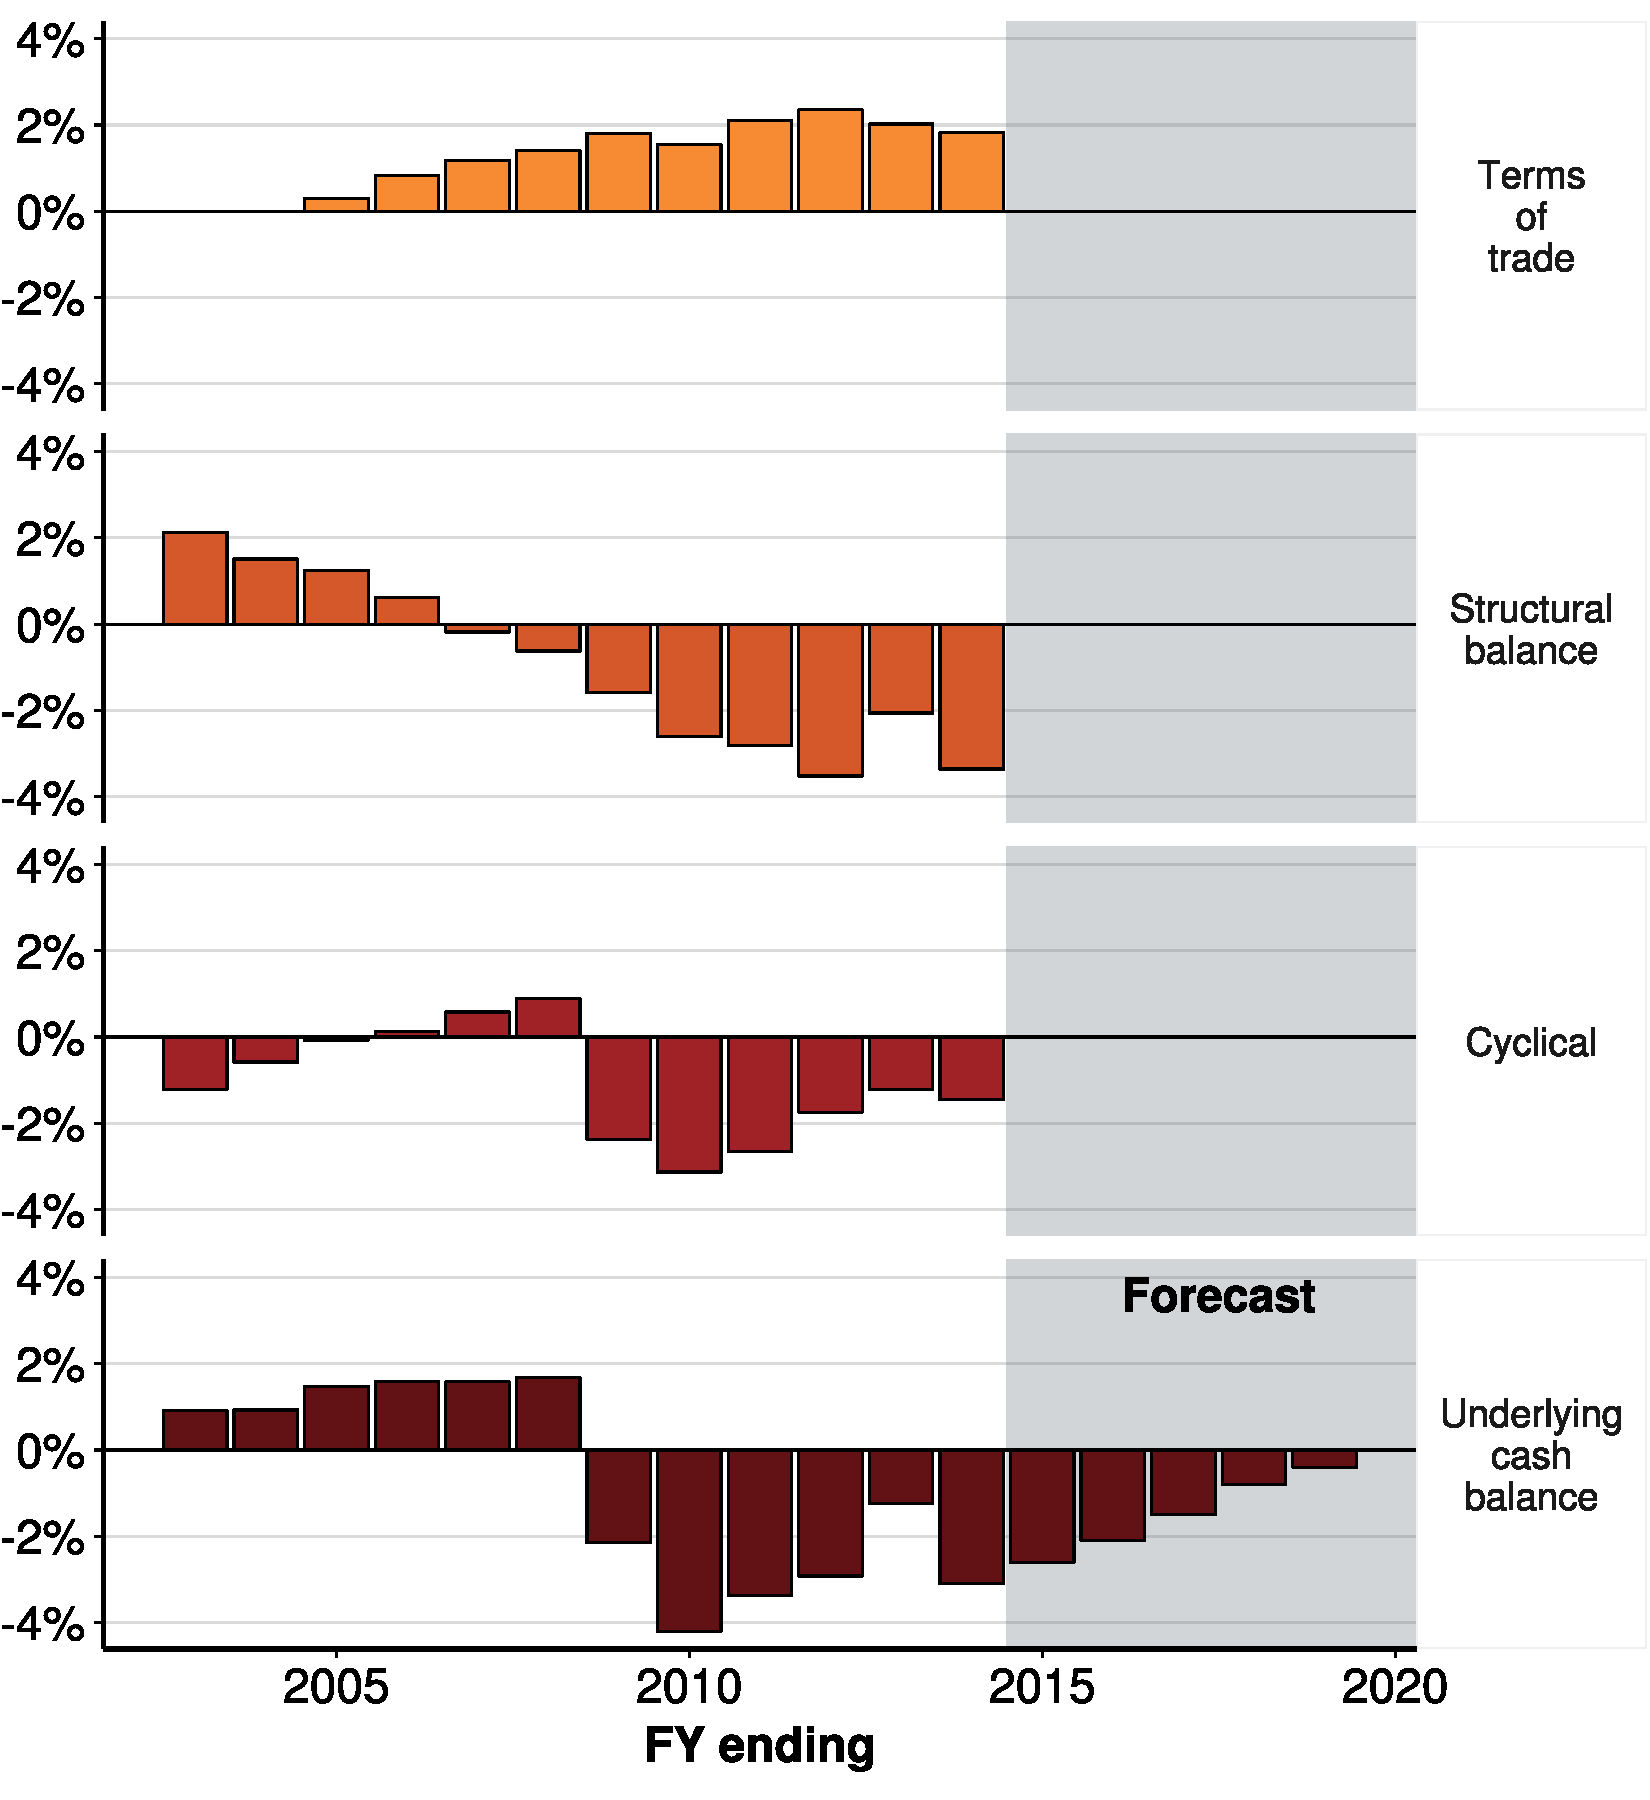
\includegraphics[width=\columnwidth]{Property-taxes/atlas/b5-figure/Figure1-1.pdf}
\fnotes{fig:PROP-1}{Immobile property includes both land and buildings; recurrent taxes on immovable property includes taxes levied regularly in respect to use or ownership of immovable property, and excludes transaction taxes on property such as stamp duty.}

\source{\textcite{OECD2015b}; Grattan analysis}
\end{figure}


\section{The property tax base is large and growing fast\label{sec:PROP-3-2}}
Property is potentially a very large tax base, worth \$8.3~trillion in June~2014. Australian land in aggregate is valued at \$4.3~trillion, and buildings and other improvements to land are worth \$4 trillion, with residential land and improvements worth about two-thirds of the total (\Cref{fig:PROP-2}). 

\begin{figure}
\captionwithunits{Australian property values grew quickly this past decade\label{fig:PROP-2}}%
{Real market value of Australian property in trillions (2014 dollars)}%
\includegraphics[width=1.2\columnwidth]{Property-taxes/atlas/b5-figure/Figure2-verso-1.pdf}
%\notes{‘Residential improvements’ consists of the value of the stock of dwelling construction, ‘Non-residential improvements’ consists of non-dwelling construction; historical figures are inflated by the Consumer Price Index to $2014. }
\source{\textcites{ABS2014e}{ABS2014h}; Grattan analysis.}
\end{figure}

Land values tend to rise at least as fast as GDP\@. Over the past 25 years land values almost tripled, growing much faster than GDP, faster than other state taxes, and faster than the GST since its introduction in 2000 (\Cref{fig:PROP-3}).\FOOTNOTE{For more detailed analysis of historical trends in individual state tax revenue growth and revenue volatility, see \Vref{appendix:PROP}.}  

\afterpage{%
\begin{figure}[!t]
\captionwithunits{Property taxes are one of the few `growth taxes'\label{fig:PROP-3}}%
{Percentage change in tax revenue for each 10~per~cent increase in national GDP, 1990-91 to 2013-14}
\makebox[\textwidth]{\includegraphics[width=1.2\columnwidth]{Property-taxes/atlas/b5-figure/Figure3-recto-1.pdf}}
\notes{‘Property levy’ shows the revenues that would have been raised with a broad-based property levy of 0.2~per~cent applied to unimproved land values had it been in place since \mbox{1990-91}; GST is for the period since its introduction in 2000-01 to 2013-14.}

\source{\textcite{ABSmultipleyears}; Grattan analysis.}
\end{figure}}


Over the longer term, property values are likely to keep rising, even if the pace of growth is slower than over the past two decades. Some of the growth over the last two decades resulted from the long-term decline in interest rates. In future, property values, and therefore revenues from property taxes, may grow more slowly.  In the long run, property prices are likely to at least keep pace with incomes, and may well rise faster, depending on population growth, household size and whether supply of new properties keeps pace with the growth in demand.\footcite[][6--7]{RBA2014SubmissionAffordableHousingInquiry}  

Revenues from property taxes tend to be less volatile than stamp duties on property sales (\Cref{fig:PROP-4}). State Treasurers dislike volatility because it makes budgeting more complex. Volatility in property tax revenues can be reduced by levying taxes on the average of recent property valuations. 

\begin{figure}
\captionwithunits{A broad based property tax would generate more stable revenues than other property taxes\label{fig:PROP-4}}%
{Standard deviation between annual revenue growth and long run average growth in Australia, (1990-91 to 2013-14), per cent}
\makebox[\textwidth]{\includegraphics[width=1.2\columnwidth]{Property-taxes/atlas/b5-figure/Figure4-verso-1.pdf}}
\fnotes{fig:PROP-4}{‘Property levy’ shows the revenues that would have been raised with a broad-based property levy of 0.2~per~cent applied to unimproved land values had it been in place since \mbox{1990-91}; GST is for the period 2000-01 to 2013-14 only, but displays similar volatility compared to state taxes assessed over this shorter period.}

\source{\textcite{ABSmultipleyears}; Grattan analysis.}
\end{figure}
%\FloatBarrier
\section{Potential revenue from a broad-based property levy\label{sec:PROP-3-3}}
A levy applied to the existing council rates base would generate substantial extra revenues for states. A relatively modest property levy, charged at a rate of \$2 for every \$1000 of unimproved land value, could raise about \$7 billion a year from 2015-16 (\Vref{fig:PROP-5}). A similar amount would be raised by a property levy charged at \$1 for every \$1000 of capital improved property value.\footnote{Capital improvements on land are investments made which increase the value of the property, particularly buildings, as well as drainage and other works. In this report, the term ‘improved value’ is used to refer to any land value definition that includes the value of improvements when assessing the value of a property.}   In comparison, state land taxes raised \$6.4 billion in 2013-14.\footcite{ABS2015h} 

\begin{figure}
\captionwithunits{A property-based levy could generate significant revenues from a modest rate\label{fig:PROP-5}}%
{Forecast annual levy revenue and 2013-14 actual collections, billions}
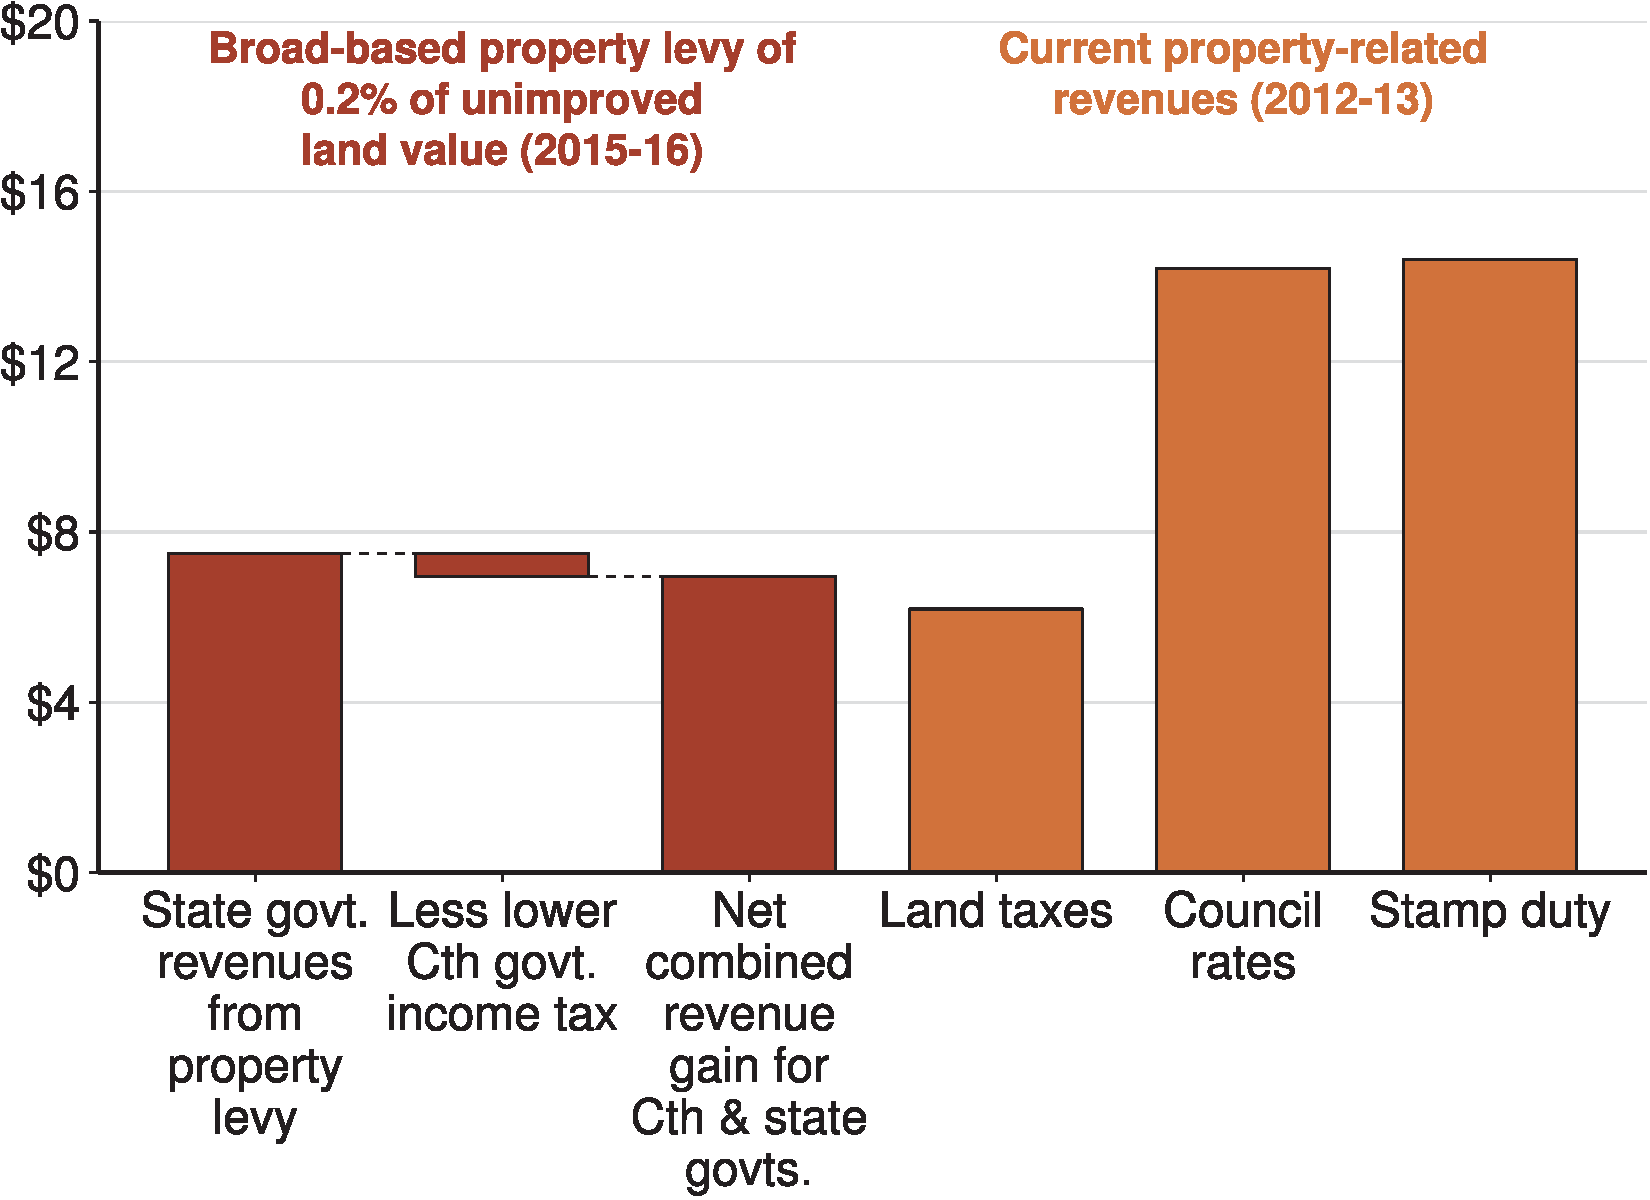
\includegraphics[width=\columnwidth]{Property-taxes/atlas/figure/Figure5-1.pdf}
\notes{Property levy revenue forecasts are for 2015-16, whereas land tax, council rates, and stamp duty revenues reflect 2013-14 collections. ABS land values for each state in the national accounts may differ, albeit not materially, from state Valuer-General figures due to different approaches, especially for residential land: see \textcite[][419]{ABS2014f}.}

\source{\textcites{ABS2014e}{ABS2014k}; \textcite{ATO2014Taxstats1112}.}
\end{figure} 

However, the property levy would reduce Commonwealth revenue by about \$0.5 billion, since property investors and firms would deduct the levy as an expense against their incomes.%
\footnote{\gao\ \textcites{ABS2013t}{ATOmultipleyears}{ABS2014k}.}

\section{\label{sec:PROP-3-4}GST redistribution due to a property levy would not excessively reduce any state’s revenue}
The Commonwealth Grants Commission (CGC) distributes GST revenues among the states to achieve what is known as \defi{horizontal fiscal equalisation}. The goal is to enable each state to deliver the same level of government services and infrastructure to its residents as other states.\footcite[][1]{CGC2015}  The CGC assesses the funds that each state would need to spend to provide the average level of services and the revenue each state would collect if it applied the average tax settings of all states. Each state then receives GST revenues to fill the gap, after accounting for other transfers it receives from the Commonwealth. 

When state governments lift their spending, it usually alters the redistribution of GST revenues. Increases in state government spending, however funded, tend to shift GST revenues towards those states and territories, such as Queensland, SA, Tasmania and the NT, where it costs more to deliver services because populations are more remote or tend to use more public services.\footnote{For example, hospital services are used more intensively by some age groups and by indigenous people.}  As a result, when total spending increases across all states, net donors such as New South Wales and Victoria tend to receive a smaller share of GST revenues, while the share of the smaller states and territories grows. The precise GST impacts depend upon how states allocate their additional spending.

GST distributions would be altered if states raised revenues through a property levy. If all States implement a property levy, then NSW, Victoria, and WA would in effect give up some of their revenues through GST redistribution, while other states and territories would receive additional GST revenues. This redistribution reflects how property levies would raise more per person in NSW, Victoria and WA, as the value of property in these states is higher. 

However, for a given scale of expenditure (and therefore revenue), a property levy would result in relatively less extreme GST redistribution than other state taxes, as \Vref{fig:PROP-6} shows. A property levy would distribute less GST money away from NSW than an increase in stamp duties would. Victoria would give up about the same percentage of new revenue, whether it raised the revenue through a property levy or through land taxes. Relative to increases in either land or payroll tax, a property levy would distribute much less GST money away from WA. 

\begin{figure}
\captionwithunits{\label{fig:PROP-6}A property levy generates less extreme GST redistribution than other major state taxes}%
{GST redistribution as a percentage of revenue raised, 2015-16}
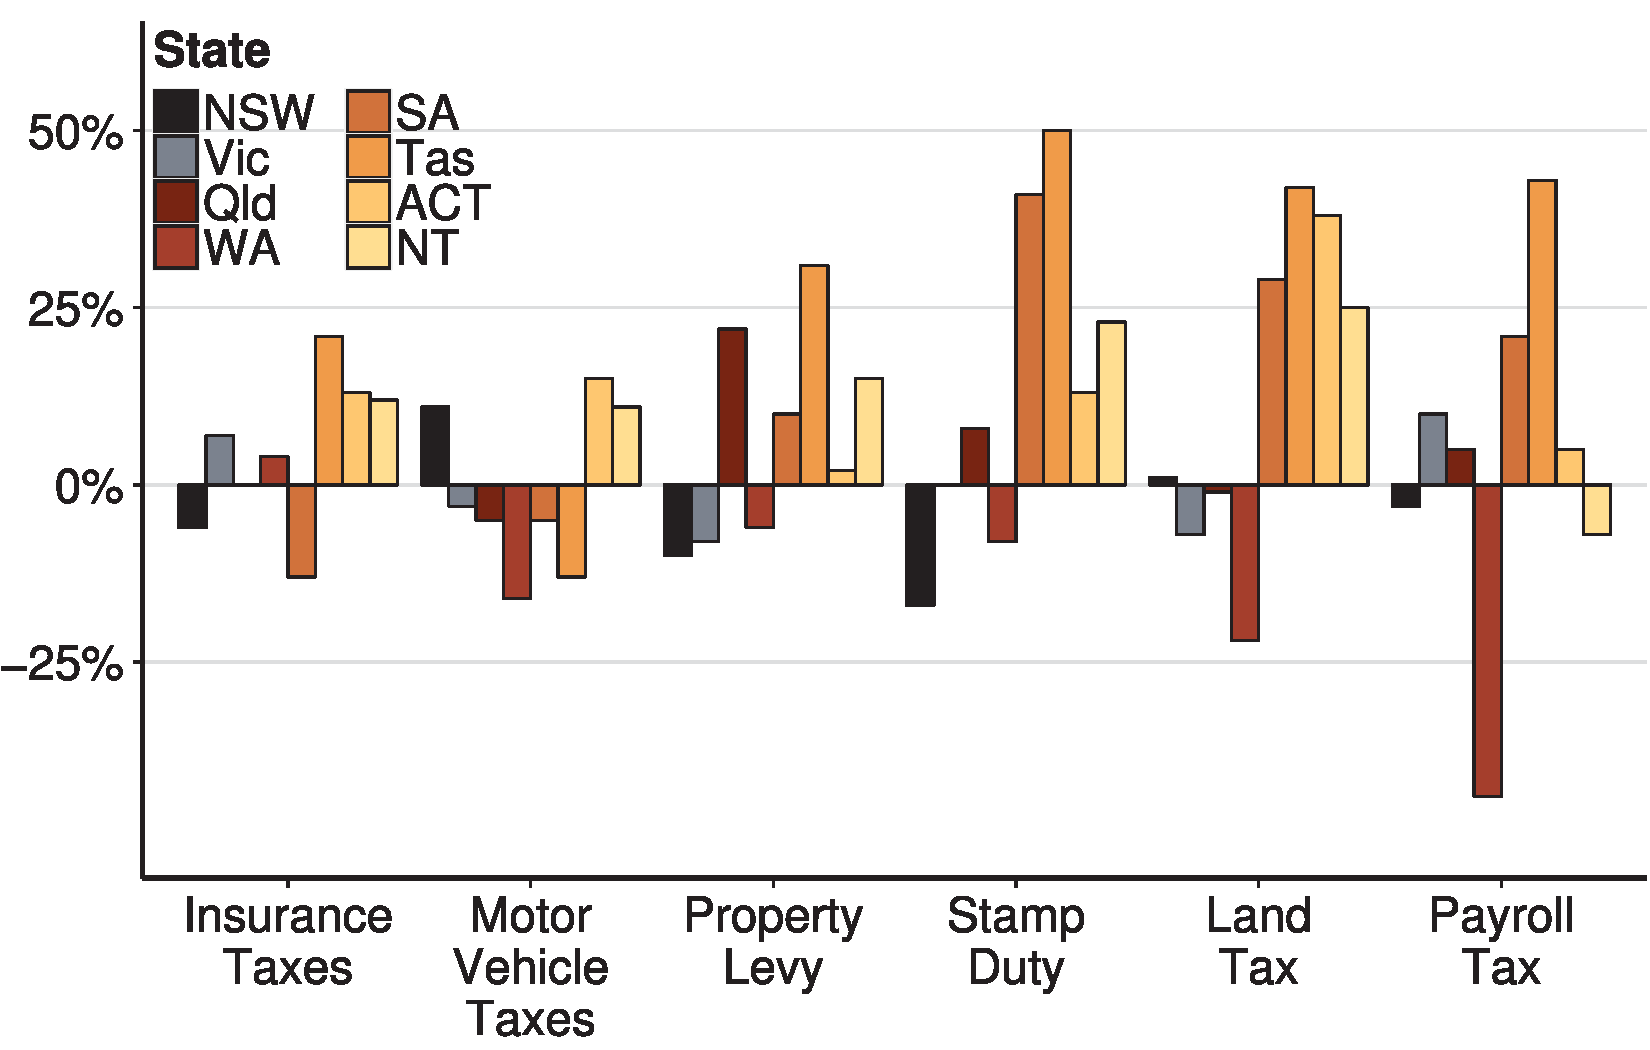
\includegraphics[width=1.0\columnwidth]{Property-taxes/atlas/figure/Figure6-1.pdf}
\notes{Assumes all states introduce the property levy; excludes any expenditure side impacts on GST revenues from states spending any extra revenues raised.}

\source{\textcite{CGC2015}; Grattan analysis.}
\end{figure}

For all states, the GST amounts redistributed would be small relative to the amount collected by a property levy. \Vref{fig:PROP-7} shows the combined effect on GST redistributions of increased spending (assuming current spending patterns), funded by a property levy imposed by all states. NSW and Victoria, with low service delivery costs and high property values, could lose at most 15~per~cent of the revenues they raise via the levy to other states. These extra revenues would mostly flow to Queensland, Tasmania, and the NT\@.

\begin{figure}
\captionwithunits{\label{fig:PROP-7}A property levy would raise slightly more per person in NSW and Victoria, but CGC redistribution would lead to similar outcomes in all States}%
{Simulated per capita annual property levy revenue, GST redistribution and net revenue impact, 2015-16}%
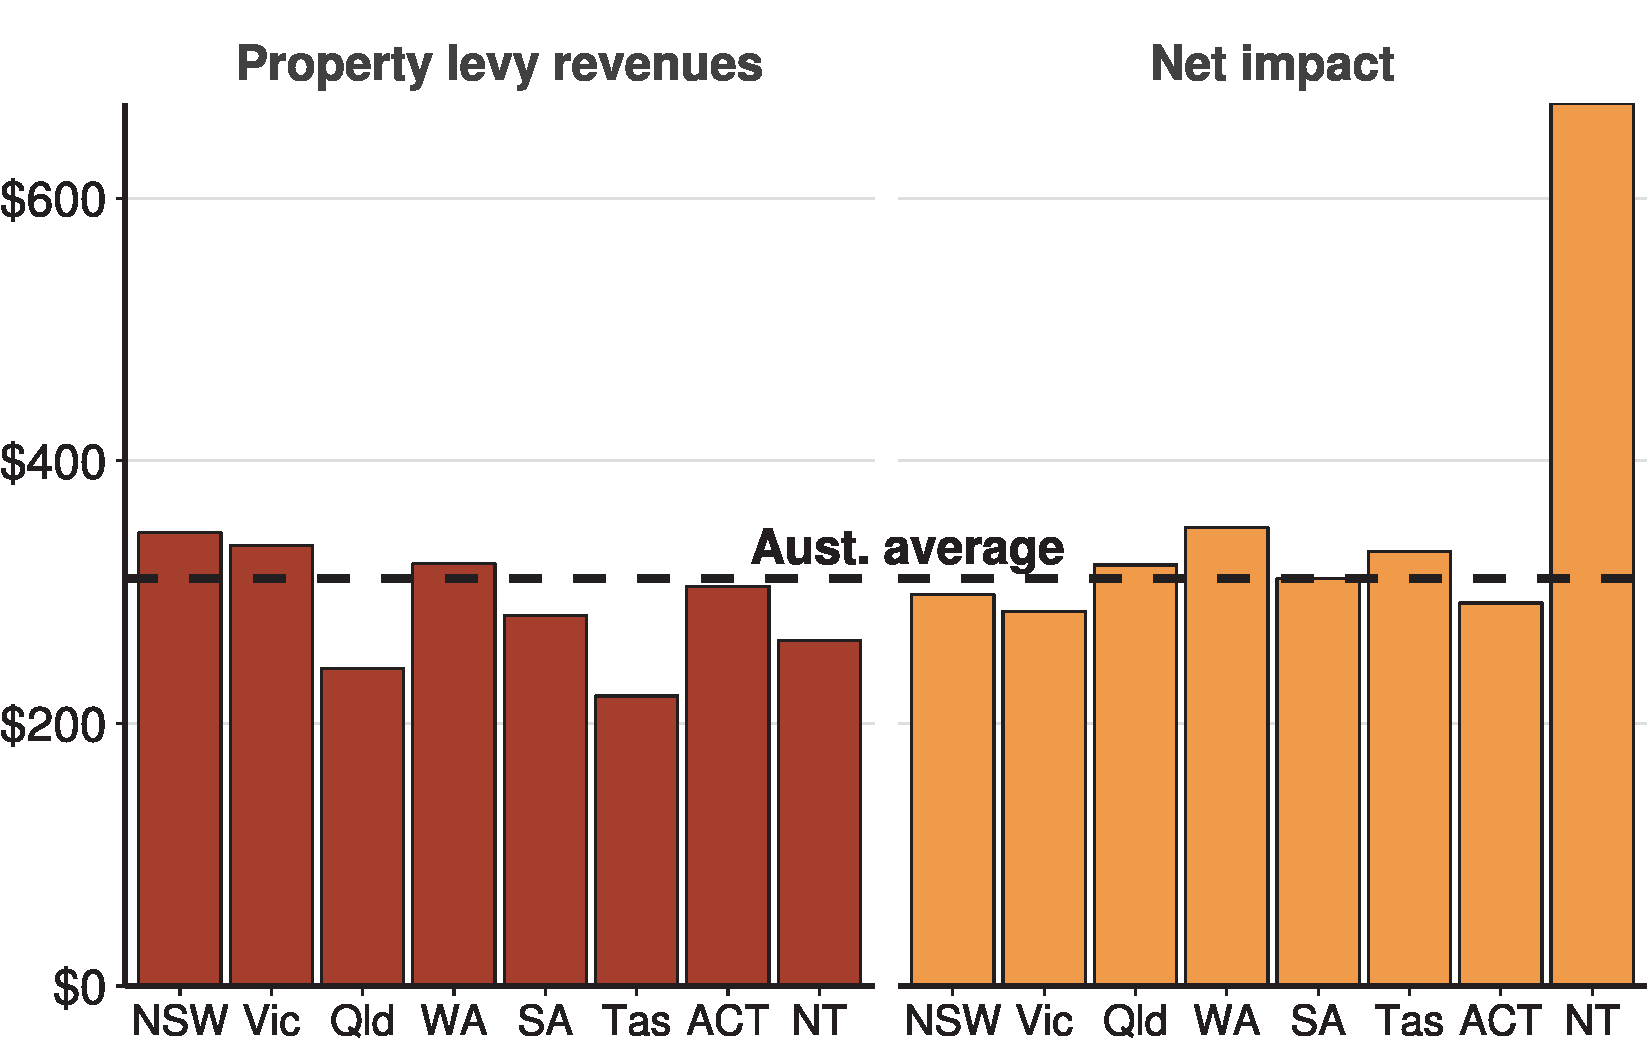
\includegraphics[width=\columnwidth]{Property-taxes/atlas/figure/Figure7-1.pdf}
\notes{Assumes a levy of 0.2\% applied uniformly to unimproved land values in each state and territory; levy is fully captured by the CGC’s methodology, and applied in 2015-16; states spend the revenues proportionate to their current expenditures; CGC assesses property levy revenues separately from state land taxes (if property levy revenues are incorporated into existing land tax assessment, this could have flow on impacts by altering the assessed land tax base).}

\source{\textcites{ABS2014}{ABS2014e}{CGC2015-Volume2}; Grattan analysis.}
\end{figure}

Because of the CGC’s methodology, GST impacts would be much smaller if only one state or a subset of states introduced the levy. For example, if NSW alone funded higher spending via the levy, it would forego about 5~per~cent of the revenues it raised. If the property levy revenues were used to fund the abolition of state stamp duties in a revenue neutral way, the GST impacts would be even smaller. NSW would replace one tax where it can raise more revenue per head (stamp duty) with another (property levy), while there would be no redistribution that reflected higher spending.  

State tax policy changes normally have a delayed effect on GST distributions. The 2015-16 GST distributions, for example, are based on data from the 2011-12, 2012-13 and 2013-14 financial years. A state property levy introduced in 2015-16 would not begin to affect GST distributions until 2017-18, and the full impact would only be incorporated in 2019-2020. 

However, if all states introduce the levy, the CGC may instead treat the new levy as if it had been in place for all of the three years of historical data used by the CGC\@. The CGC used this approach in 2006 when the states agreed to abolish certain state taxes.\footcite[][23]{CGC2015-Volume2}  

%\begin{bigboxC*}
\cleardoubleevenstandardpage
\begin{lultrabox}{Taxes and economic growth}{box:PROP-1}%
All taxes reduce growth because they distort decision making by households and firms.

Taxes influence household decisions about how much to save and spend, how many hours to work and what to invest in. Similarly, taxes affect the decisions of companies about how much and what to produce, how much labour and capital to employ and where to locate.

Welfare is reduced when people and firms make decisions different to the ones they would have made if taxes were not in place. This is measurable as a loss in economic output.  Taxes also generate an administrative burden and encourage people to expend effort trying to avoid them. The diversion of resources to these unproductive activities reduces economic growth. 

But some taxes drag on growth more than others. As a general rule, taxes on more mobile assets such as foreign financial capital are more likely to change behaviour and therefore harm growth compared to the taxation of less mobile assets such as land. Taxes on transactions, such as stamp duties, are particularly inefficient taxes. They distort the decision to buy and sell assets and so distort the optimal allocation of resources. 

Economic models have been used to estimate the loss of efficiency from a range of taxes. \Vref{fig:PROP-8} shows the estimated loss of economic activity, or marginal excess burden, from each dollar increase in each tax.

There are potentially sizeable gains to productivity and economic growth if governments shift some of the tax burden towards more efficient taxes.

\begin{figure}[H]
\captionwithunits{Some taxes drag less on economic growth than others\label{fig:PROP-8-left}}%
{Loss of economic activity}
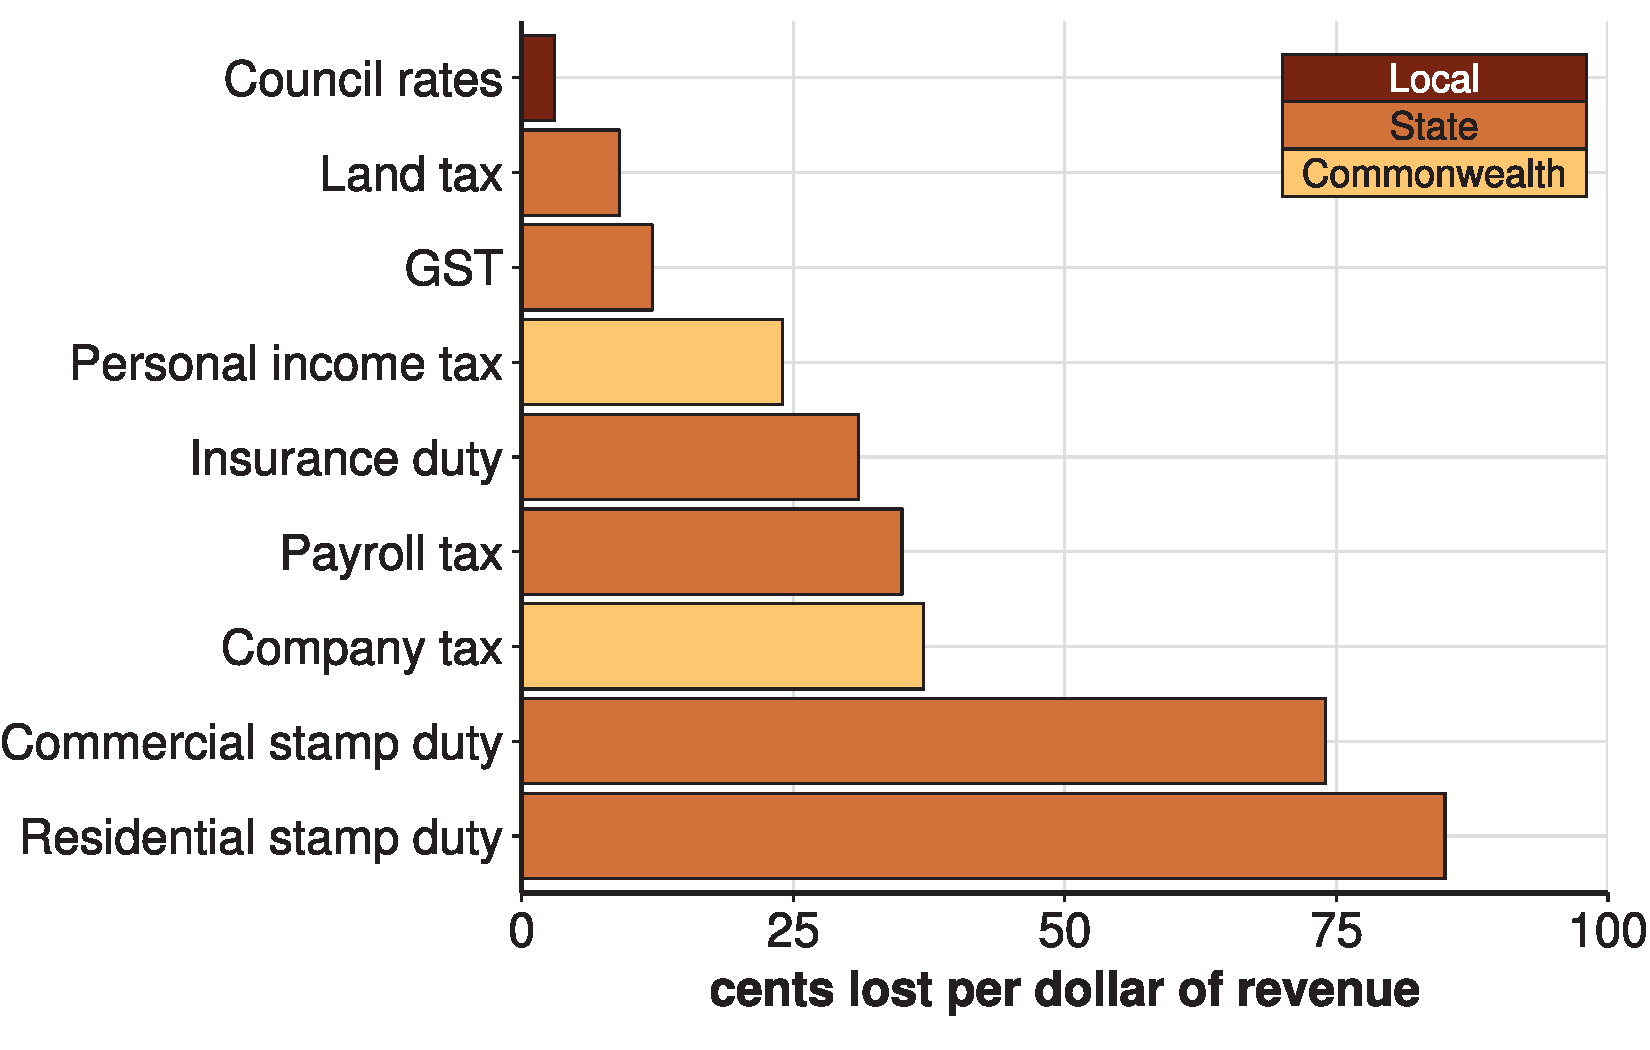
\includegraphics[width=\linewidth]{Property-taxes/atlas/b5-figure/Figure8-1.pdf}

\notes{All marginal excess burden estimates are from \textcite{KPMGEconotech2011-GST} other than council rates that come from the KPMG modelling for \textcite{HenryTaxReview2010}. These estimates are broadly consistent with Treasury estimates which evaluated a smaller range of taxes \textcite{CaoHoskingKouparitsasEtAl2015}. This more recent work suggests that the economic burden of broad-based land taxes may be even lower, with a marginal excess burden of $-\!\text{10}$\,c, since the revenue from foreign owners of land would exceed the economic costs imposed on Australian residents.}
\end{figure}
\end{lultrabox}
\begin{rultrabox}{Taxes and economic growth}{box:PROP-1-right}%
All taxes reduce growth because they distort decision making by households and firms.

Taxes influence household decisions about how much to save and spend, how many hours to work and what to invest in. Similarly, taxes affect the decisions of companies about how much and what to produce, how much labour and capital to employ and where to locate.

Welfare is reduced when people and firms make decisions different to the ones they would have made if taxes were not in place. This is measurable as a loss in economic output.  Taxes also generate an administrative burden and encourage people to expend effort trying to avoid them. The diversion of resources to these unproductive activities reduces economic growth. 

But some taxes drag on growth more than others. As a general rule, taxes on more mobile assets such as foreign financial capital are more likely to change behaviour and therefore harm growth compared to the taxation of less mobile assets such as land. Taxes on transactions, such as stamp duties, are particularly inefficient taxes. They distort the decision to buy and sell assets and so distort the optimal allocation of resources. 

Economic models have been used to estimate the loss of efficiency from a range of taxes. \Vref{fig:PROP-8} shows the estimated loss of economic activity, or marginal excess burden, from each dollar increase in each tax.

There are potentially sizeable gains to productivity and economic growth if governments shift some of the tax burden towards more efficient taxes.

\begin{figure}[H]
\captionwithunits{Some taxes drag less on economic growth than others\label{fig:PROP-8}}%
{Loss of economic activity}
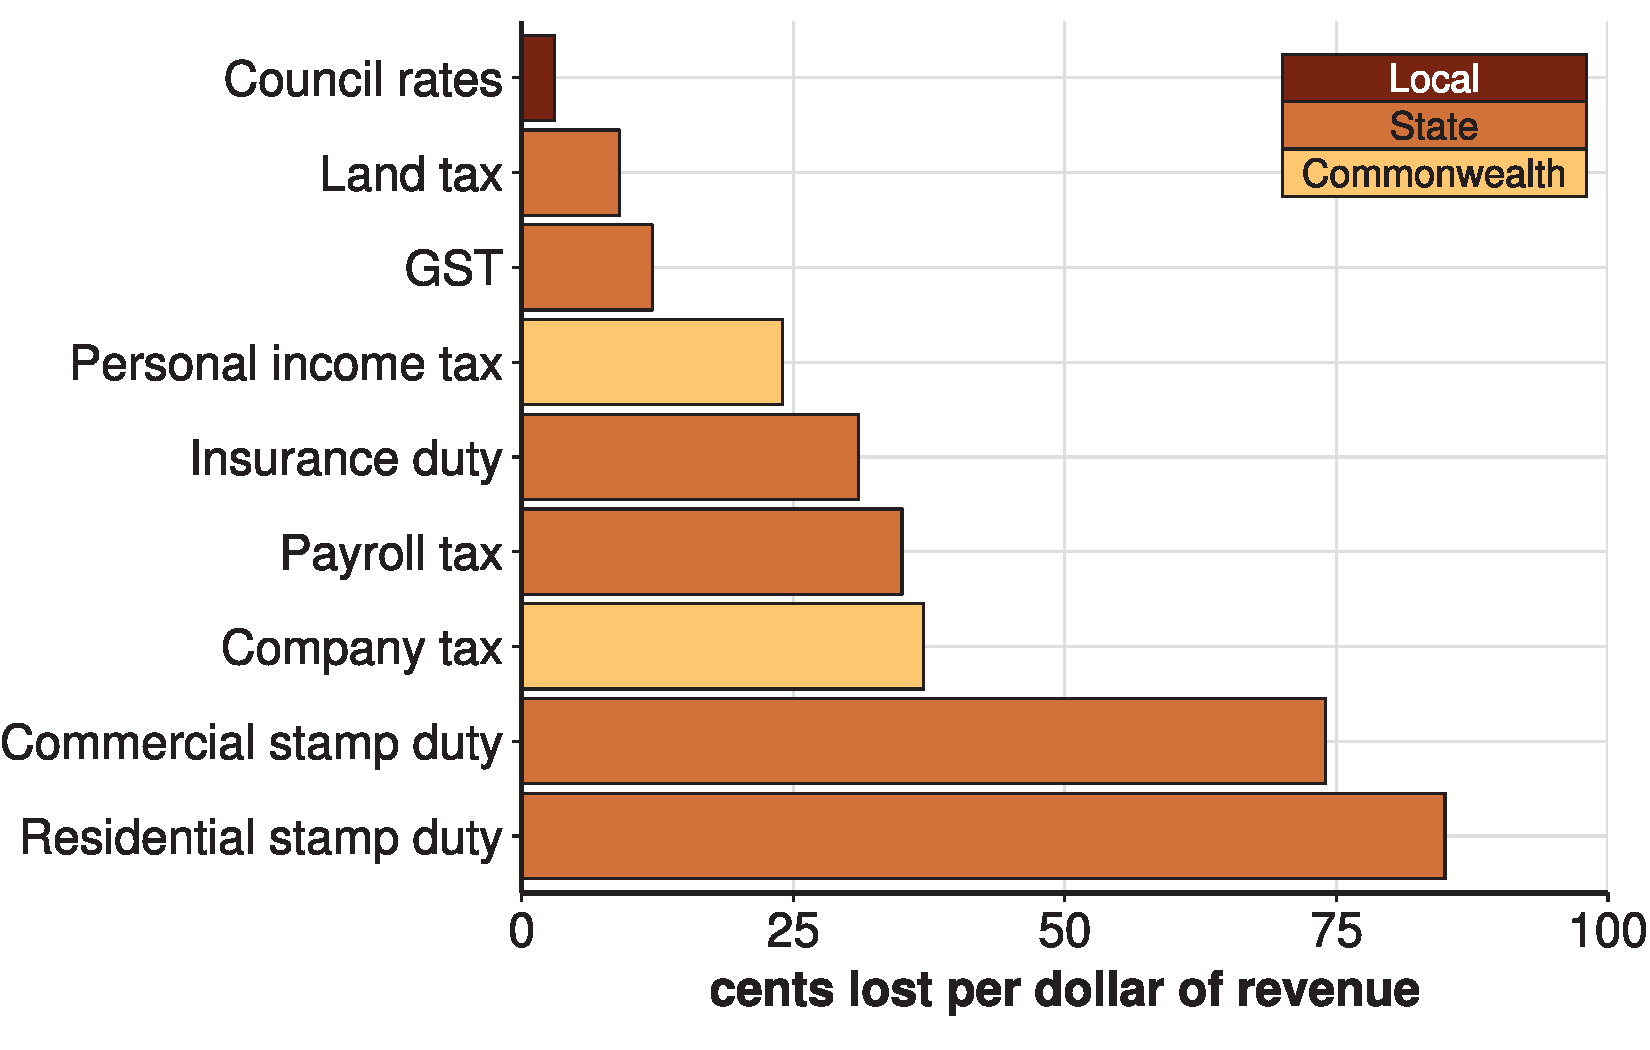
\includegraphics[width=\linewidth]{Property-taxes/atlas/b5-figure/Figure8-1.pdf}

\notes{All marginal excess burden estimates are from \textcite{KPMGEconotech2011-GST} other than council rates that come from the KPMG modelling for \textcite{HenryTaxReview2010}. These estimates are broadly consistent with Treasury estimates which evaluated a smaller range of taxes \textcite{CaoHoskingKouparitsasEtAl2015}. This more recent work suggests that the economic burden of broad-based land taxes may be even lower, with a marginal excess burden of $-\!\text{10}$\,c, since the revenue from foreign owners of land would exceed the economic costs imposed on Australian residents.}
\end{figure}
\end{rultrabox}


\makeatletter\@openrighttrue\makeatother
\chapter{Property taxes are relatively efficient}
Property taxes – which are levied on the value of property holdings – are the most efficient taxes available to the states. Governments that want to increase the amount of revenue they raise will harm growth less with property taxes than with most other taxes. Unlike capital, property is immobile – it cannot shift offshore to avoid higher taxes. The risks of multinational tax avoidance, the increasing mobility of capital, and the increasing value of residential property relative to incomes, should make property taxes a priority in any tax reform. 


%
\section{Broad-based land taxes are the most efficient taxes}
All taxes drag on economic growth. But some taxes do so less than others (\Vref{box:PROP-1}). Broad land taxes are the most economically efficient taxes because they do not discourage working or investing. Unlike capital or labour, the supply of land is fixed. Someone must use the land: it cannot be moved away. 

Land taxes do not distort decisions about land use, provided they apply in a way that the landowner can’t avoid.\footcite[][247]{HenryTaxReview2010}  For example, a constant rate land tax applied to the unimproved value of all land prevents landowners from reducing their liability to such a tax by changing how they use their land. An empty block of land would pay the same tax even after it was developed. 

Broad-based land taxes are much more efficient than stamp duties (\Vref{box:PROP-1}). Given estimates of the inefficiency costs of stamp duties, abolishing stamp duties in all states and replacing them with a broad-based land tax could add \$9 billion a year to GDP.\footnote{\gao\ \textcites{KPMGEconotech2011-GST}{ABS2015h}.}

Land is typically valued in its unimproved state.\footnote{In this working paper, the term \defi{unimproved value} is used to capture a range of land value definitions, such as unimproved value, and site value, among others. Although there are differences in the definitions, they all capture the value of land separate from the value of major capital improvements, such as buildings. For example, see \textcite[][153]{HefferanBoyd2010}.}  The unimproved value of a parcel of land does not include the value of improvements, such as the construction of buildings on it. Instead, it depends on the most valuable use of the land that would generate the highest return – as residential housing, farmland, an office tower, an industrial site, and so on – subject to the land uses permitted under planning laws.\footnote{Land use restrictions tend to reduce land values where they prevent land being used for its’ first and best use. For example, \textcite{KulishRichardsGillitzer2011} find that residential building height restrictions result in lower land prices closer to the CBD where the height restriction is binding \textcite[][11]{KulishRichardsGillitzer2011}. However land use restrictions also tend to increase land values for land approved for certain uses by increasing the scarcity of that type of land. See \textcite{Brueckner2007} for a theoretical overview of the impact of land usage policies on land prices.}

Economic theory predicts that a tax on unimproved values – applied equally to all land – would result in land prices being lower than otherwise. Yet rents should remain constant as the land tax doesn’t affect how land is used (see \Cref{sec:PROP-7-1}).\footnote{Land taxes are capitalised into land values (\textcite[][247--248]{HenryTaxReview2010}).}   

Land taxes can also capture some of the value created by public investment such as transport infrastructure. These gains are today taxed very lightly. Owner occupied housing is exempt from the two taxes that would capture some of the value of these gains: capital gains tax and land tax. 

Property prices in major Australian cities have risen faster in suburbs closer to the CBD than in those located further out, which mainly reflects increases in the price of land, not what has been built on it.\footcite[][22]{KulishRichardsGillitzer2011}  Faster growth in land values in inner-city locations in Australian cities reflect, in part, the value of public transport, government-funded schools, parks and other public amenities, as well as proximity to employment opportunities.\footcite[][87]{KellyDonegan2015}

\section{Property taxes at low rates are a little less efficient than taxes on land, but are still attractive\label{sec:PROP-4-2}}
Although they are less efficient than land taxes, property taxes -- which include the value of capital improvements such as buildings -- are still very efficient taxes. An OECD report found that reducing income taxes by 1~per~cent of GDP, and increasing taxes on immobile property (both land and buildings) by the same rate would improve long run GDP per head by 2.5 percentage points.\footcite[][58]{JohanssonHeadyArnoldEtAl2008}

Property taxes are a little less efficient than land taxes because property taxes also tax the returns on capital invested to improve the property. This results in fewer improvements being made to land, such as fewer buildings, than would otherwise be the case. In the longer term, a portion of the property tax will be passed on to property users through higher rents for rental housing or for firms leasing premises, for example. The effect will flow on to other prices.

\section{\label{sec:PROP-4-3}Economic costs are particularly small with low tax rates}
Under the low property tax rate we propose, any economic costs are likely to be very small. The economic costs of a tax tend to be much lower for low tax rates.\footcite[][18]{KPMGEconotech2011-GST}  On plausible assumptions, a property tax of 0.1~per~cent of property value would tax the return on capital improvements at about 0.8~per~cent.\footnote{Assuming an average nominal pre-tax rate of return on capital of 12~per~cent. The tax rate on capital improvements would rise to 1.4~per~cent for an investment with a pre-tax rate of return on capital of only 7~per~cent.}  To put this in context, a landlord doing capital improvements of \$100,000 would need to collect a mere \$8 extra a month in rent to recoup the costs of the tax.\footnote{This figure is independent of the rental return rate adopted.}

Unlike many other forms of capital investment, which can move to avoid higher taxes, most existing capital improvements to land, such as buildings, cannot be moved. Therefore taxing improvements on land would be unlikely to affect the existing stock of capital improvements. Along with the low tax rate we propose, this means that the effect of a property tax on new capital invested would be modest, as \Vref{box:PROP-2} illustrates.  

\setlength{\currentparskip}{\parskip}
\afterpage{%
\begin{lultrabox}{A modest property tax has a similar impact on property \newline development returns as a land tax}{box:PROP-2}
To understand how a property tax would affect returns on property development compared to a land tax, we consider a hypothetical investment.

We compare a property tax of 0.1~per~cent on improved value with a land tax of 0.2~per~cent on unimproved value. These taxes would raise about the same revenue each year. 

We consider an investor who buys land intending to develop it by investing in new capital improvements. We calculate the rate of return on the total investment given various levels of new capital improvement. \Cref{fig:PROP-9} on the facing page \DEVIATION{To ensure boxheight identical} shows that returns are very similar under the alternative regimes, even in cases where improvements account for most of the property value after redevelopment. 

The differences only become material at much higher rates of tax. For example, comparing a property tax rate of 1~per~cent to a land tax rate of 2~per~cent (both of which would raise about \$70~billion), the annual rate of return on new improvements worth twice the value of the land would be 0.3~percentage points lower. The difference in the rates of return would be greater – about 0.8~percentage points – for capital investment typical for apartments, where the building cost can be 10~times the land value.

\begin{figure}[H]
\captionwithunits{A low rate tax on improvements has little impact on returns on the total investment\label{fig:PROP-9-left}}%
{Annual rates of return after taxes on property for redeveloped property}
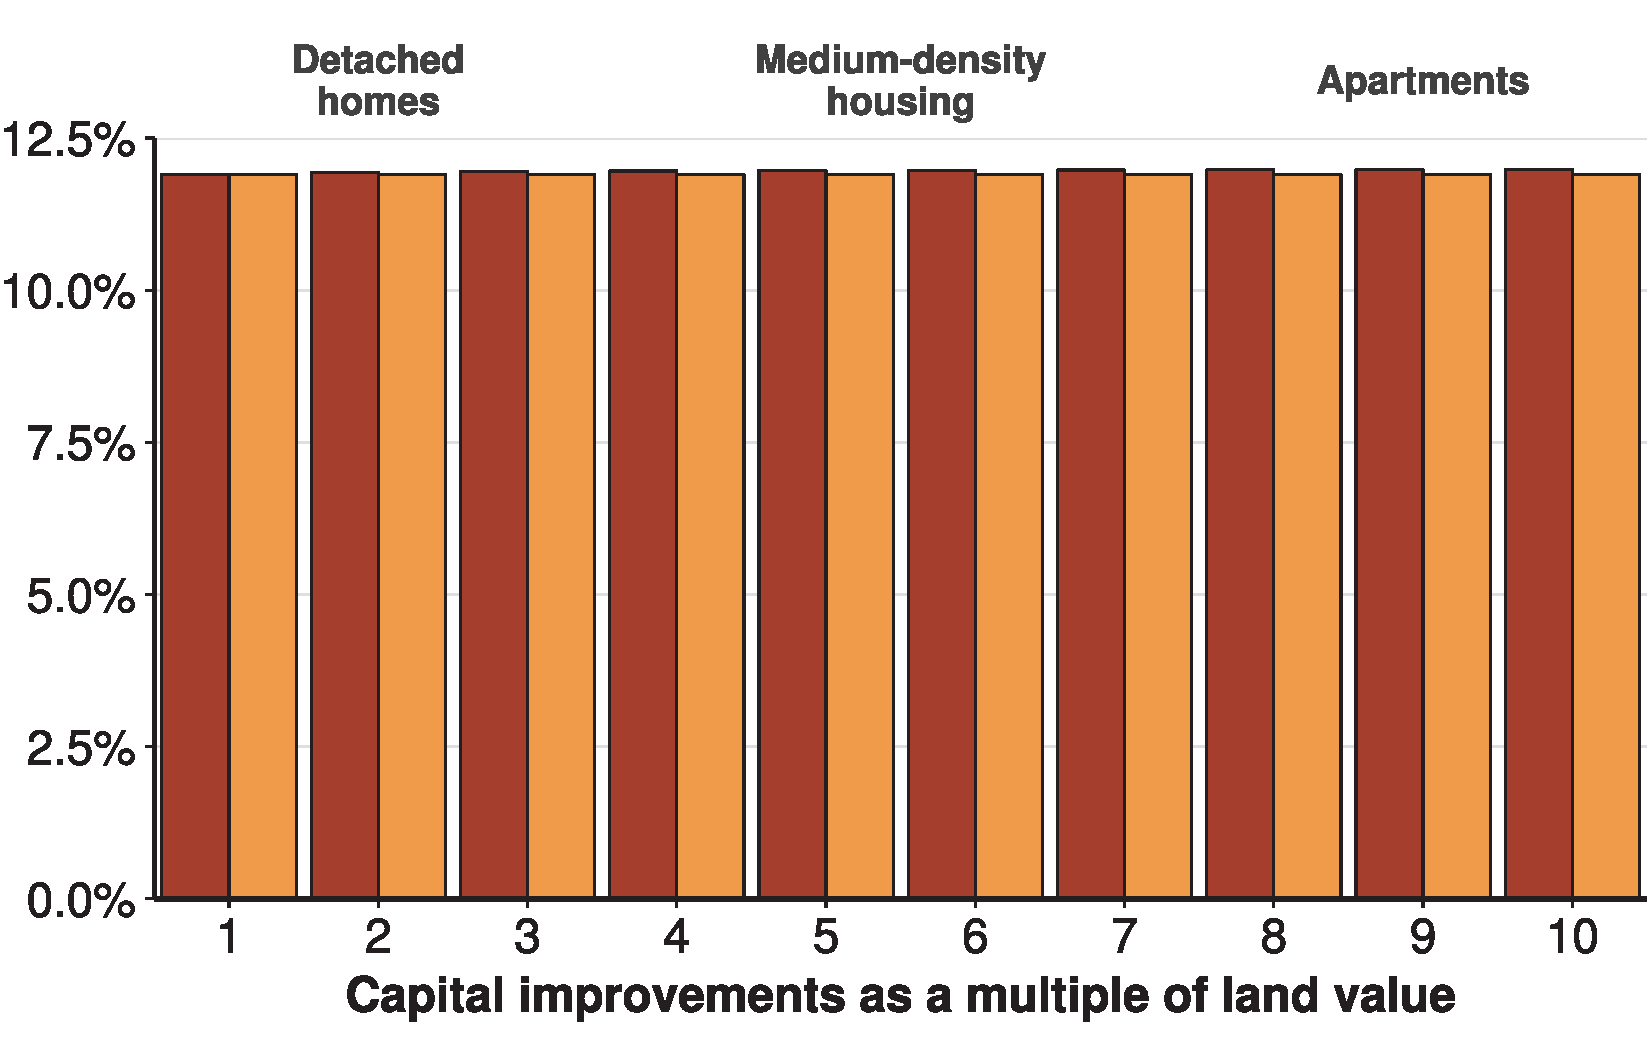
\includegraphics[width=\linewidth]{Property-taxes/atlas/figure/Figure9-1.pdf}
\notes{Based on a property tax rate of 0.1~per~cent, and a land tax rate of 0.2~per~cent. Assumes a pre-tax rate of return on the total investment of 12~per~cent.}

\source{Grattan analysis.}
\end{figure}%
\end{lultrabox}
\begin{rultrabox}{A modest property tax has a similar impact on property \newline development returns as a land tax}{box:PROP-2-right}
To understand how a property tax would affect returns on property development compared to a land tax, we consider a hypothetical investment.

We compare a property tax of 0.1~per~cent on improved value with a land tax of 0.2~per~cent on unimproved value. These taxes would raise about the same revenue each year. 

We consider an investor who buys land intending to develop it by investing in new capital improvements. We calculate the rate of return on the total investment given various levels of new capital improvement. \Cref{fig:PROP-9} on the facing page shows that returns are very similar under the alternative regimes, even in cases where improvements account for most of the property value after redevelopment. 

The differences only become material at much higher rates of tax. For example, comparing a property tax rate of 1~per~cent to a land tax rate of 2~per~cent (both of which would raise about \$70~billion), the annual rate of return on new improvements worth twice the value of the land would be 0.3~percentage points lower. The difference in the rates of return would be greater – about 0.8~percentage points – for capital investment typical for apartments, where the building cost can be 10~times the land value.

\begin{figure}[H]
\captionwithunits{A low rate tax on improvements has little impact on returns on the total investment\label{fig:PROP-9}}%
{Annual rates of return after taxes on property for redeveloped property}
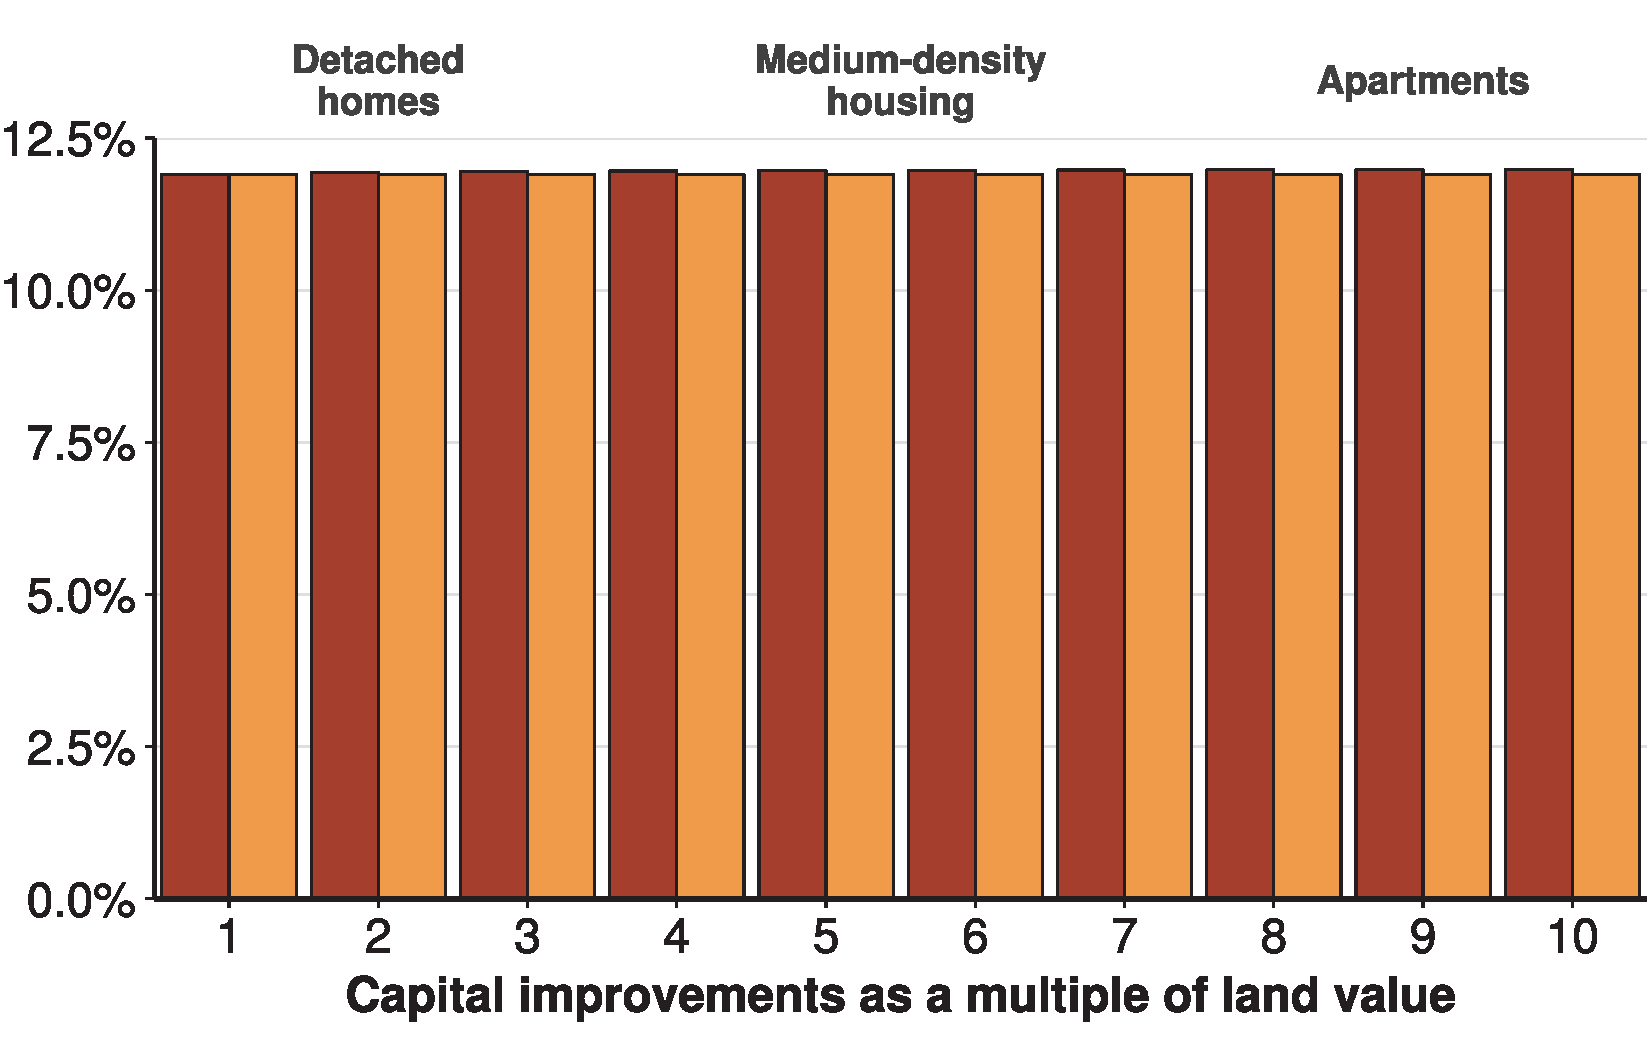
\includegraphics[width=\linewidth]{Property-taxes/atlas/figure/Figure9-1.pdf}
\notes{Based on a property tax rate of 0.1~per~cent, and a land tax rate of 0.2~per~cent. Assumes a pre-tax rate of return on the total investment of 12~per~cent.}

\source{Grattan analysis.}
\end{figure}%
\end{rultrabox}
}

While there are no estimates from Australia, several overseas studies have found that property taxes have relatively low economic costs. A survey of US property taxes found that every dollar collected reduced economic output by just 6 to 16 cents. On these estimates, property taxes are efficient relative to other state taxes such as payroll tax and stamp duty, as \Vref{fig:PROP-8} shows. Since taxes tend to be more efficient when levied at low rates, even these estimates overstate the economic costs of a proposed property tax of 0.1~per~cent of property value – a tax rate 16 times smaller than those investigated in the US studies.\footnote{The weighted average of U.S. state property taxes in the year 2000 investigated by these studies is equivalent to an annual tax rate of 1.56~per~cent of property values.}  

\chapter{Legislative basis for property tax reform\label{chapter:PROP-5}}
Additional property taxes should build upon existing tax bases. State and local governments already levy two types of property taxes: land tax and council rates. 

All states and territories except the Northern Territory levy land taxes. They base the taxes on the value of the land without capital improvements such as buildings.  Land taxes exempt owner-occupied housing and most agricultural land – more than half of all land by value (\Vref{fig:PROP-2}). 

The other property tax base is the municipal rates levied by local councils, usually based on improved values. Because very few properties are exempt from this tax it is a much better base from which to charge a property levy.\footnote{Land taxes also usually exempt much Commonwealth and State-owned land, and land used by public hospitals, libraries, cemeteries, charities, religious organisations, universities, schools and foreign embassies. See \textcite[][105]{productivity2008assessing}.}  Some States have already levied emergency services levies on this municipal rate base.

\section{State land taxes are a compromised tax base}
Existing state land taxes generate much less revenue than a broader-based land tax would. States raised \$6.4 billion from land taxes in 2013-14.\footcite{ABS2015h}  Exempting the family home from land tax excludes about 75~per~cent of the value of residential land, and state government budgets forgo about \$5 billion in revenue.\footnote{\textcites[][261]{HenryTaxReview2010}[][24]{KellyMaresHarrisonEtAl2013}. Even though owner-occupied housing accounts for 75~per~cent of all residential land, imposing land tax on it would only raise \$5 billion as it would be taxed at comparatively low rates under the highly progressive rates of land tax currently in force.}  Exemptions for agricultural land remove almost a further 10~per~cent of land by value from the land tax base (\Cref{fig:PROP-2}).\footcite[][260]{HenryTaxReview2010}

States also apply substantial tax-free thresholds based on total landholdings before any tax is levied. These thresholds range from \$25,000 in Tasmania to \$600,000 in Queensland and further reduce state revenues from land taxes.\footcite[][31--33]{Treasury2014-Interstate-Comparison-Taxes1415}   

\phantomsection
Land taxes are also levied on a progressive scale\label{paragraph:PROP-land-taxes-levied-on-progressive-scale} so that people with larger land holdings pay a higher rate of land tax per dollar value of land owned. Progressive rates reduce the efficiency of the ideal land taxes that were discussed in Section 4. They discourage larger landholdings and partly explain why small investors dominate Australia’s rental housing market, with relatively few landlords owning a large number of properties.\footcites{Berry2000}{WoodOngStewart2010}[][261]{HenryTaxReview2010}

For example, a small investor with a single investment property in Sydney built on land valued at \$750,000 pays land tax of \$5,508 in 2014. By comparison, a large investor owning ten such properties pays \$133,432 in land tax, or \$13,343~per~property.\footcite[][31--33]{Treasury2014-Interstate-Comparison-Taxes1415} 

Land tax exemptions also make the system more difficult to administer and for landowners to comply with.\footcite[][261]{HenryTaxReview2010}  Tax-free thresholds and progressive rate structures provide landowners with incentives to break up their land holdings and adopt complex ownership structures in order to reduce their land tax payments. Time and resources spent by firms to manage more complex structures are a burden on productivity.\footcite[][157]{GabbitasEldridge1998}  Tax authorities use grouping provisions to overcome incentives to fragment land holdings, but impose additional costs in administering them. 

Exempting owner-occupied housing is also very regressive. The exemption for the family home benefits households in the top income quintile by almost \$2000, but benefits households in the bottom income quintile by just \$400.\footcite[][27]{KellyMaresHarrisonEtAl2013}   

State land taxes could be an efficient tax base provided that exemptions, thresholds and progressive tax rates were abolished. Yet extending the existing land tax base to cover owner-occupied residential property and agricultural land would be politically difficult, and is likely to be portrayed as favouring businesses at the expense of consumers.

Similarly, removing tax free thresholds and shifting to a single flat land tax rate assessed at the property level would result in much lower tax liabilities for large landholders. Again, such a reform could well be portrayed as unfair: favouring a small number of wealthy landlords while increasing land tax liabilities for smaller landholders. 

\begin{table}
\captionwithunits{Approaches to valuing properties for council rates vary\label{tbl:PROP-1}}%
{Property value bases that can be used to set council rates in each state}
\begin{tabularx}{\columnwidth}{>{\bfseries}lX}
%
\toprule
\textbf{State} & \textbf{Basis for council rates} \\%[0.5\baselineskip]
\midrule
\textbf{NSW} & Unimproved  \\[0.5\baselineskip]
\textbf{QLD} & Unimproved  \\[0.5\baselineskip]
\textbf{VIC} & Either unimproved or capital improved  \\[0.5\baselineskip]
\textbf{WA} & Capital improved  \\[0.5\baselineskip]
\textbf{SA} & Either unimproved or capital improved \\[0.5\baselineskip]
\textbf{TAS} & Either unimproved or capital improved  \\[0.5\baselineskip]
\textbf{NT} & Unimproved  \\[0.5\baselineskip]
\textbf{ACT} & Unimproved  \\%[0.5\baselineskip]
\bottomrule
\end{tabularx}
\notes{‘Unimproved’ refers to a set of land valuations that capture the value of the land only. ‘Capital improved’ refers to valuations that capture the value of the land and significant capital improvements made to that land, such as buildings.}

\source{\mbox{\textcites{productivity2008assessing}{mangioni2014re}{Treasury2014-Interstate-Comparison-Taxes1415}}.}
\end{table}

Municipal rates regimes vary across councils. Councils may levy a fixed charge, a variable rate based on property values, or a combination of the two. In some states, councils determine the tax base for rates by choosing between measures of unimproved or capital improved property values (\Cref{tbl:PROP-1}).\footcite[][198]{productivity2008assessing}  Despite these differences, a state government levy added to council rates would be relatively simple to administer. In practice a government could set a state-wide rate, with the council rate as an additional charge that varies by council.

There are no constitutional barriers to states adopting the council rates base to raise revenues. Although councils set and often collect rates, they are ultimately levied under the authority of state government legislation. 

\begin{table}
\captionwithunits{Property-based emergency services levies are a template for property tax reform\label{tbl:PROP-2}}%
{Structure for state property-based emergency services levies}
\begin{tabularx}{\columnwidth}{lXXXXr}
\toprule
& \multicolumn{2}{c}{\begin{tabular}{c} \textbf{Property} \\ \textbf{value used} \end{tabular}} & \multicolumn{2}{c}{\textbf{Levy structure}} &  \\ 
\cmidrule(lr){2-3}\cmidrule(lr){4-5} 
\textbf{State}  & \begin{tabular}{@{}>{\centering}p{\linewidth}@{}} \textbf{Land} \\ \textbf{only} \end{tabular} & \begin{tabular}{@{}>{\centering}p{\linewidth}@{}}  \textbf{Land \&} \\ \textbf{building} \end{tabular} & %
	\begin{tabular}{@{}>{\centering}p{\linewidth}@{}}  \textbf{Fixed} \\ \textbf{charge} \end{tabular} & \begin{tabular}{@{}>{\centering}p{\linewidth}@{}}  \textbf{Variable} \\ \textbf{rate} \end{tabular}  & \begin{tabular}{@{}r@{}} \textbf{Collection} \\ \textbf{authority} \end{tabular}\\
\midrule
Vic & \cellNo & \cellYes & \cellYes & \cellYes & Councils \\
WA rural & \cellYes & \cellNo & \cellYes & \cellYes & Councils \\
WA metro & \cellNo & \cellYes & \cellYes & \cellYes & Councils \\
SA & \cellNo & \cellYes & \cellYes & \cellYes & State govt.\\
ACT & \cellYes & \cellNo & \cellNo & \cellYes & State govt. \\
\bottomrule
\end{tabularx}
\notes{The ACT funds fire services via a levy based on unimproved property values for commercial property only, with a fixed charge for residential and rural land. The ACT also uses the average of unimproved land values over the past 3 years; WA sets minimum charges for the total levy collected on each property, which act as a de facto fixed charge for some ratepayers.}

\source{\textcites{Victoria2014}{Revenue2015}{ACT2004}{WesternAustralia2015}}
\end{table}

Governments in Victoria, South Australia, Western Australia and the ACT already use the council rates base for state-wide property-based levies to fund fire and emergency services. These levies provide a template for reform. They are charged as a share of land or property values. The levy rates are set at the state level. In Victoria and Western Australia (but not South Australia), notices of liability are issued as part of council rates notices, and levies are collected by councils and passed on to state governments (\Vref{tbl:PROP-2}). Over time a large state property levy might lead to centralised collection of both property levy and council rates through state revenue offices.

\section{\label{sec:PROP-5-2}Council rates are a better taxation base than state land taxes}
Local councils levy rates on the value of unimproved land, and in some states, on capital improved values. Rates are applied to all properties within a council area with few exemptions. There are no exemptions for owner-occupied housing or agricultural land and constant rates apply from the first dollar of property value with no minimum threshold. The largest exemption from council rates is for some non-profit, non-government organisations such as charities, schools and public hospitals.\footnote{For example, the City of Gosnells estimated the value of the rates revenue foregone by WA councils from exemptions to charities in WA at \$6.5 million, or 0.7~per~cent of total state-wide council rates revenue for 2005-06. See \textcite[][107]{productivity2008assessing}.}

Council rates are levied at the same rate per dollar of land value of a property, regardless of the overall size of ratepayers’ total property holdings, and so do not discriminate against large property investors.\footnote{In Victoria, for example, most councils determine rates on the basis of the assessed capital value of the property. See \textcite[][154]{HefferanBoyd2010}.}  

\chapter{Key design choices for a property levy}
A modest levy on property values could generate significant revenues for states and territories, with less drag on economic activity than other available state taxes.

\section{A flat rate levy on property values, with no fixed charge, is the simplest approach\label{sec:PROP-6-1}}
The levy could be designed in a number of ways. A flat tax rate on property values would be the simplest. The levy would consist of a flat rate charged per dollar of property value, with no fixed charge per property. It would apply equally to all land, regardless of land use, and from the first dollar of property value with no minimum threshold. It would be assessed separately on each property owned, as currently occurs with council rates, using existing Valuer-General valuations. 

A flat rate with no fixed charge would be more equitable than council rates and the existing state emergency services levies which both include a fixed or minimum charge. These reflect the fee-for-service implicit in charges for council services and emergency services. Yet these levies are inherently regressive as they fall more heavily on the less well off.\footnote{\textcite[][139]{productivity2008assessing}  notes that ‘other things equal, imposing a minimum (or fixed) charge makes rates regressive (or less progressive) than otherwise’.}  A state property levy aimed at raising general revenue should have no fixed charge.

Recent Commonwealth and state tax reviews have considered levying land tax with higher tax rates for land with a higher value per square metre.\footcites[][265]{HenryTaxReview2010}[][41]{GovernmentSouthAustralia2015-State-Tax-Review-Discussion-Paper}  Yet the problems with progressive rates probably outweigh the benefits.

On the plus side, a progressive rate structure captures more of the spill-over benefits of public investments in infrastructure, such as transport infrastructure, parks, schools, and libraries that increase nearby property values. Higher taxes on vacant property in expensive inner-city locations might also speed development as higher property taxes increase holding costs.\footcite{WoodOngCigdemEtAl2012}  A progressive tax rate would also be popular with politically powerful farming lobbies, since most farmland would be taxed at a low rate.

The progressive rate also reflects – albeit very approximately – the progressive nature of state stamp duties. If a property levy aims not only to raise additional revenue but to replace existing stamp duties, a progressive rate on the levy might provide less of a bonus to the owners of highly priced properties that currently incur high stamp duties when purchased.

However, a progressive rate property levy would still lead to different tax treatments for properties that at present incur the same stamp duty. For example, with tax calculated on the price of land per square metre, the owners of small inner city apartments would pay much more than they do under the replaced stamp duties. The owners of similarly priced outer suburban houses would pay much less. 

To the extent that a property levy is a tax on wealth, a levy charged at a progressive rate would treat people with similar wealth differently. 

An increasing marginal tax rate based on the value of land per square metre would make a property levy more complex to administer. It would require more accurate and reliable land valuations since higher levy rates would compound any errors in the land valuation process. 

A progressive tax rate should only be applied to unimproved land values, as otherwise it would significantly discourage investing in improvements. However, a progressive rate compounds the administrative complexities of taxing unimproved values: unimproved values are hardest to determine accurately where land values are highest, and hence the consequences of disputed valuations are worth more.

\section{\label{sec:PROP-6-2}A levy rebate would reduce the burden on low wealth property holders, but would significantly reduce revenue}
Providing an exemption, or rebate, for the first portion of property tax liability would make the levy more progressive with respect to household wealth.\footnote{For example, see \textcite[][8]{SlackBird2014}.}  Households with lower wealth tend to own lower value homes, so the rebate would reduce the average property tax rate applied to low wealth property owners.  

However, such a rebate could easily halve the revenue raised from the levy. A \$500 rebate on a property levy applied to unimproved land values would mean that no landowner would pay the property levy on landholdings worth less than \$250,000. Such a rebate would exclude about half of all residential properties in NSW, even if property owners could only claim the rebate in respect of one property.\footnote{Based on a property levy 0.2~per~cent of unimproved land value, and median residential land values supplied by NSW Treasury.}

A rebate would also provide incentives for landowners to fragment holdings across different legal entities in order to make use of multiple rebates, as currently occurs with state land taxes.

\section{\label{sec:PROP-6-3}The levy should be applied to land values, but a levy on capital improved property values is a good alternative}
The property levy could be applied to only the unimproved value of land, or to the combined value of land and buildings. Although a tax on unimproved value is theoretically better, it increases implementation problems, and the practical impacts on investment of a levy on capital improved values would be small. 

A levy on unimproved land values is preferable because it does not discourage investing in improvements. While many councils levy rates on capital improved values, state Valuer-Generals maintain comprehensive registers of unimproved land values to determine state land tax liabilities.\footnote{Councils in all states except WA currently have the option to levy rates based on land values (\Vref{tbl:PROP-1}).}  A levy on unimproved land values could be applied universally, with the levy listed as a separate item on ratepayers’ council rates notices.

A levy on unimproved values would also make it easier to use increased levies to replace stamp duties over time. Replacing stamp duties would require higher rates of tax – potentially about 0.4~per~cent of unimproved values. 

While it is less economically efficient, a levy based on property values is easier to administer and would be a good alternative. A tax on improved values would still be much more efficient than a stamp duty, and most other state taxes. Capital improved property values are easier to determine since market sales and rental data are more readily available. Effective property taxes require up-to-date, transparent and accurate property valuations. The recent shift towards capital improved values for council rates in some states reflects difficulties in determining the true unimproved value of land, especially in dense urban areas where there are few, if any, market sales of unimproved land.\footcites[][24]{Ombudsman2005}[][153]{HefferanBoyd2010}

\section{\label{sec:PROP-6-4}An annual charge is simpler than a capitalised charge collected on sale}
Some have suggested capitalising the property tax for all landowners, and collecting the capitalised charge (potentially including accrued interest) only when the property is sold.  This would mimic the political advantages of current stamp duties: they are paid less often, and only when the vendor is cashed up from a recent sale. Because the amount payable depends on how long the vendor has owned the property, a capitalised charge would reduce the problems of the current stamp duty regime, which discourages more frequent property turnover.

Yet this design has a number of problems. Above all, it would be complex to explain, and therefore unattractive to politicians. 

A capitalised charge would also lead to significant increases in state gross debt as governments would collect promises of future payment rather than cash, unless interest was charged. 

The approach also presents problems similar to those that arise with capital gains tax. Unless there is an interest charge on accrued tax then the property holder receives an interest free loan until the property is sold. The investor has large incentives not to sell, which locks people into holding properties – the precise problem that makes stamp duties so inefficient. 


\section{Levy deferral for pensioners: managing the impact for income-poor, asset-rich owner-occupiers\label{sec:PROP-6-5}}
However, capitalising the charge may be a good option to manage the impact on the relatively small number of income-poor, asset-rich owner-occupiers.

A property levy would pose difficulties for people who are asset-rich but income-poor, especially retirees who have limited incomes but own their own home. Retirees who want to stay in their homes should be able to do so. Many are emotionally attached to them. They provide continued access to social networks, and leaving them often carries large financial and emotional costs. 

One option is to provide concessions to property owners with low incomes. State governments typically provide rebates on council rates to pensioners and other concession cardholders.\footnote{In most cases, states provide a fixed rebate on council rates, and reimburse councils for the foregone rates revenues. Many councils also offer an additional fixed rebate on municipal rates for pensioners and concession card holders. In most cases, property-owning pensioners still have some residual rates liability after these concessions are applied.}  Similar concessions also apply in those states that charge property-based fire services levies. 

However, exempting or providing concessions to asset-rich but cash-poor landowners would be unfair to younger taxpayers. It also ignores the substantial resources of some retirees. Concessions based on pension eligibility are already poorly targeted: many wealthier Australians receive the Age Pension. Of mature age households with a million dollars of net assets, about 80~per~cent receive welfare benefits.\footcite[][37]{DaleyMcGannonSavageEtAl2013BalancingBudgets}  

A fairer approach would be for state governments to allow these asset-rich, income-poor households to defer paying the levy until they sell their property. Deferral arrangements are already available for seniors paying council rates in South Australia, Western Australia and the ACT (\Vref{box:PROP-3}).\footcite{Brownfield2014} 

The amount could accrue as a debt against the property, with an appropriate caveat registered at the Land Title Office. Interest should be charged on the balance to reflect the cost of deferral. A safety net might be provided by a stipulation that the debt cannot account for more than 20~per~cent of the value of the property, and would be non-recourse.\footnote{Under a non-recourse loan, the creditor cannot claim any other assets of the borrower if the borrower defaults and the collateral is insufficient to repay the debt.}  This would protect ratepayers from longevity risks – where individuals live longer than expected and the debt comes to exceed the value of the property as interest charges continue to compound over time. 

In reality, very few retirees would use this safety net. At the tax rates proposed, 30 years of deferred levy and the accumulated interest would still only be 5~per~cent of the property value.\footnote{A 0.1~per~cent levy on property value, with payment deferred for 30 years would result in a deferred charge equivalent to 4~per~cent of the property value, including deferred interest. This assumes a 7~per~cent nominal interest rate and 3~per~cent annual growth in nominal house prices. With a 10~per~cent nominal interest rate, the deferred charge would be equivalent to 7~per~cent of the property value.}  

Yet the safety net could become more important if the levy rate were raised in future -- to fund the abolition of stamp duty, for example. 

Levy deferral schemes should be statewide since state governments would ultimately receive the revenues. A statewide scheme could also incorporate existing council rate deferral schemes and be extended to state-based emergency services levies.\footnote{State governments typically reimburse councils for the rate revenue foregone under council rate deferral programs.} 


\begin{smallbox}[p]{The Postponement of Rates Scheme (SA)}{box:PROP-3}
The Postponement of Rates Scheme, operated by South Australian councils, allows retirees to postpone payment of council rates. Similar schemes operate in Western Australia and the ACT\@. The scheme is designed to help elderly ratepayers to finance their rates payments by unlocking the value of home equity. Such households may own their own homes and are therefore asset-rich, but on low incomes.

Eligible ratepayers can postpone a portion of the rates applied to their principal place of residence. Any rates after the first \$500 each year can be postponed. The scheme is only available to ratepayers that own their property alone, or with their spouse.

Ratepayers incur interest on the outstanding debt, which compounds monthly. The interest rate is set at the average borrowing costs for councils in that year, which was 6~per~cent in 2013-14. Ratepayers receive an update on their postponed rates debt, and any accrued interest, as part of their rates notices each year. The accrued debt is payable when the property is sold or transferred to someone else and no surviving spouse remains living in the house. 

To be eligible, a ratepayer must be over 60 years of age and work less than 20 hours a week in paid employment. Ratepayers must also have at least 50~per~cent equity in their property after accounting for any outstanding mortgage debt if the mortgage was registered before 25 January 2007. 
\end{smallbox} 

\chapter{The levy would not impose unreasonable burdens\label{chapter:PROP-7}}
\section{The levy would reduce property values, but would have little impact on rents\label{sec:PROP-7-1}}
An increase in property taxes usually reduces property values, all else being equal, with little impact on rents. Potential buyers of property will reduce how much they are willing to pay by the future cost of property tax payments.\footnote{There is considerable literature documenting the capitalisation of property taxes into land values. For example see \textcites{Oates1969}{oates2009simple}. \textcite[][22]{WoodOngCigdemEtAl2012} adopt a similar approach to estimate the impact of the Henry Review recommendations on land values in Victoria.}  Therefore the tax liability is capitalised into the property value. For example, a 0.2~per~cent levy on unimproved land values would be expected to reduce land values by between 3 and 6~per~cent.\footnote{The impact of the tax on land values depends upon the discount rate adopted.  For example, a property levy would lower land values by 6~per~cent with a discount rate of 2~per~cent, but by only 3~per~cent if a 6~per~cent discount rate is adopted. This analysis assumes a levy of 0.2~per~cent on land values only.}

A levy on unimproved land values would have no impact on rents. If a landowner tried to pass on the tax by charging higher rents, some people would decide not to rent, thereby lowering rental demand and causing rents to fall back again.

A levy on capital improved property values might lead to small rent rises, since it would discourage some investment in new improvements and therefore affect the supply of housing. Over time, landlords are likely to pass on to renters some of the additional costs that the levy imposes on improvements. Yet as \Vref{fig:PROP-9} shows, the impact on rents is likely to be small as the levy would have only a very small impact on the returns that accrue from investing in new improvements. For example, if a landlord sought to pass through the full cost of the levy after investing \$500,000 in developing improved land priced at \$500,000, it would increase the annual rent by 1~per~cent, or \$10 a week.\footnote{Rents would rise by 1.3~per~cent for a real rental yield (excluding any capital gains) of 4~per~cent. For a rental yield of 7~per~cent, the percentage increase in rents drops to 0.7~per~cent. Both examples reflect a property levy of 0.1~per~cent of capital improved property values.}  In reality the impact would be smaller as only a small share of the levy would be passed through because new improvements are a small share of the total housing stock.

\section{Costs for property owners would be manageable}
A homeowner would pay a levy of \$772 a year on the median Sydney house valued at \$772,000, or \$560 a year on the median Melbourne home valued at \$560,000. The average levy burdens on households in other major Australian cities would be lower (since property prices are lower), and lower still in regional areas (\Vref{tbl:PROP-3}).

\begin{table}[h]
\captionwithunits{Costs for property owners would be manageable\label{tbl:PROP-3}}%
{Property levy payable on the average home by capital city, (2015-16 dollars)}
% Table generated by Excel2LaTeX from sheet 'Sheet1'
\begin{tabularx}{\columnwidth}{lRR}
\toprule
\textbf{City} & {\textbf{Median dwelling price}} & \textbf{Property levy per year} \\
\midrule
\textbf{Sydney} & {\$772,200} & \$772 \\
\textbf{Melbourne} & {\$560,000} & \$560 \\
\textbf{Brisbane} & {\$455,000} & \$455 \\
\textbf{Perth} & {\$510,000} & \$510 \\
\textbf{Adelaide} & {\$405,000} & \$405 \\
\textbf{Hobart} & {\$315,500} & \$316 \\
\textbf{Darwin} & {\$515,000} & \$515 \\
\textbf{Canberra} & {\$535,000} & \$535 \\
\bottomrule
\end{tabularx}
\notes{Based on a 0.1~per~cent levy on capital improved property values, applied to the median prices of homes in major Australian cities, as at June 30, 2015.}

\source{\textcite{RPCoreLogic2015-Capital-city-dwelling-values-rise}; Grattan analysis.}
\end{table}

The average burden of the levy on each property owner would be
smaller than existing council rates for most owners (\Vref{fig:PROP-10}).\footnote{This analysis assumes a levy of 0.2~per~cent on land values only. The results
would be broadly similar for a levy on capital improved property values of around
0.1~per~cent.}
Property holders with higher incomes would pay more in absolute
terms than those with lower incomes. Those with higher incomes
tend to own more valuable homes, and are more likely to own an
investment property.

\begin{figure}
% \captionsetup{margin={0cm,-\extraWd}}
\captionwithunits{\label{fig:PROP-10}The property levy would be less than council rates for most property owners}%
{Expected property taxes payable by income decile (2011-12 dollars)}
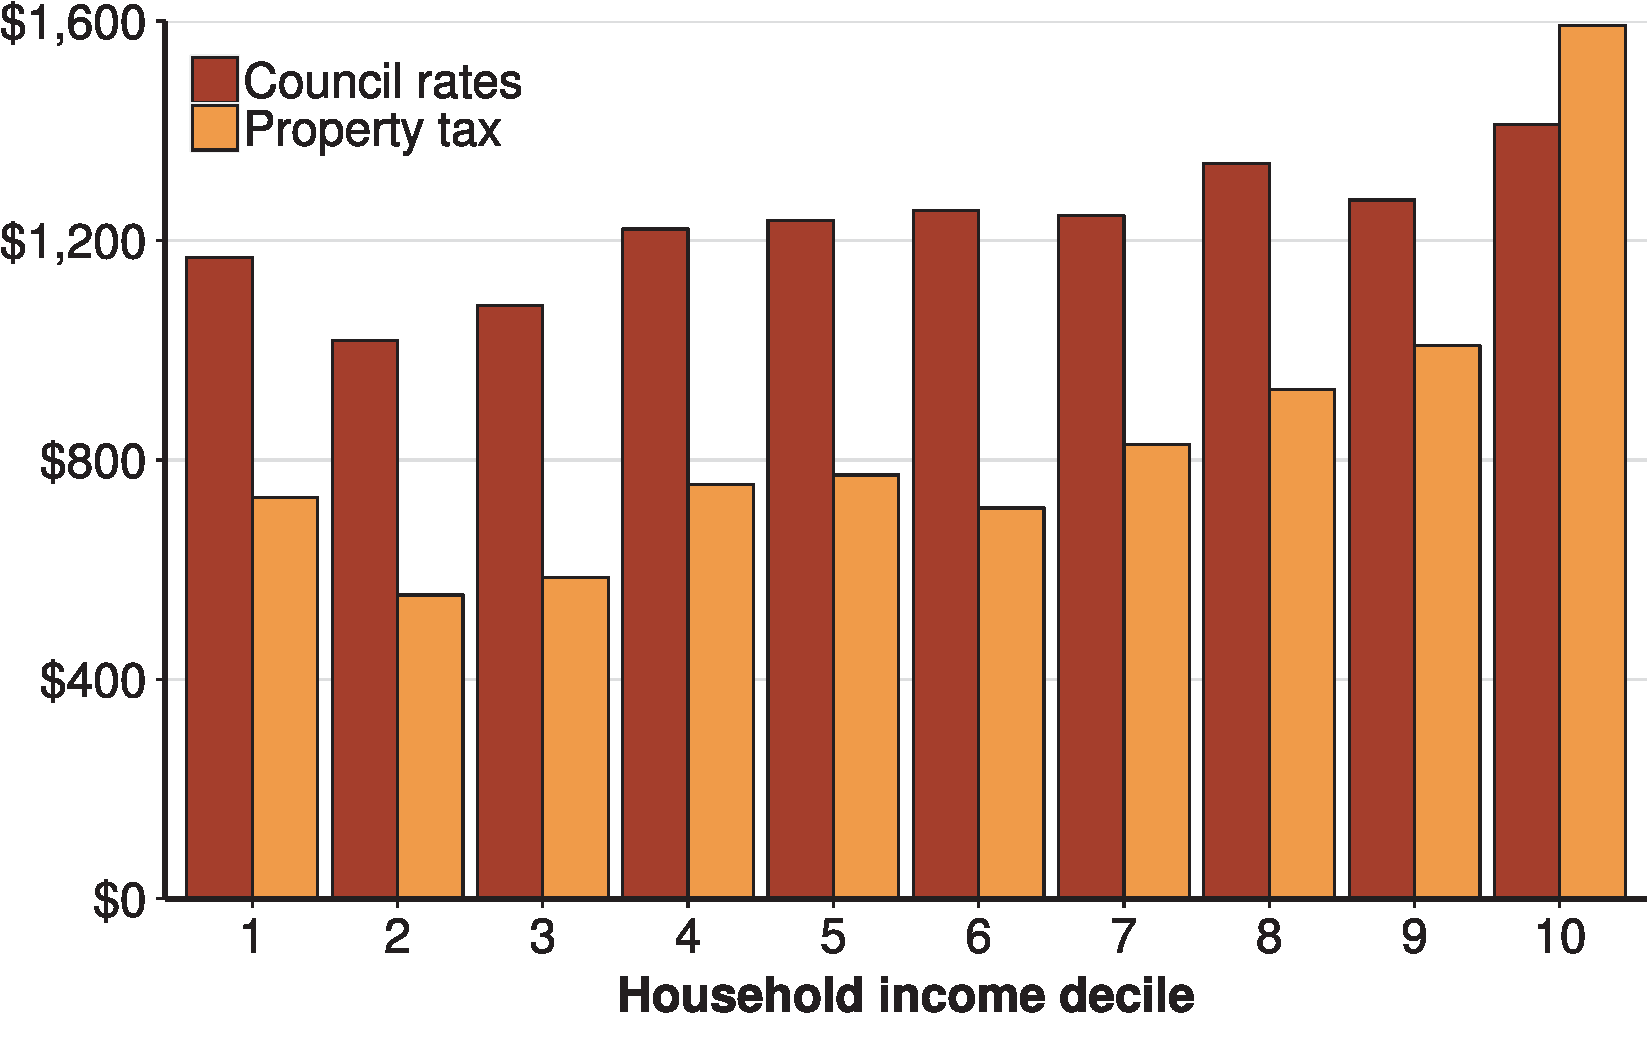
\includegraphics[width=\columnwidth]{Property-taxes/atlas/figure/Figure10-1.pdf}
\fnotes{fig:PROP-10}{Simulated impact of applying a 0.2~per~cent levy to unimproved land values; average rates and levy costs are calculated based only on those households within the disposable income decile that would pay the levy; households reporting negative household disposable income and negative net wealth are excluded from the analysis; council rates include all charges, net of rebates, but exclude water charges; deciles are grouped by equivalised disposable (\ie~post tax) income of each household.}

\source{\textcite{ABS2013t}; Grattan analysis.}
\end{figure}

\subsection{Impact on those worst off}
The impact of revenue measures on the poorest households is a particular concern.\footcite[][21]{DaleyMcGannonSavageEtAl2013BalancingBudgets}  While measures of inequality traditionally focus on income, material wellbeing depends upon both income and accumulated wealth. Assessing taxpayers’ capacity to pay should consider the ability of households to draw on their net wealth, or generate income from their assets.\footcite[][180]{OECD2013d}  This approach is especially important when considering wealth taxes such as a property levy. Consequently, the distribution of both wealth and income are relevant in assessing the impact of a property levy. A particular concern is the impact on households that are in the bottom 20~per~cent of the income distribution and have low net worth.\footnote{The ABS adopts the concept of household net worth, rather than household wealth, in the Survey of Income and Housing. See \textcite[][19]{ABS2014l} for a detailed discussion on this issue.} 

A property-based levy would fall largely on households with higher net worth, reflecting their greater property holdings (\Vref{fig:PROP-11}). Households that are both income and asset poor would, on average, pay almost no levy. By contrast, households ranked among the top 20~per~cent by net worth – of at least \$640,000 – would pay an average of \$1933 annually.\footnote{The equivalent net worth figure for a two adult household in the top income net worth quintile would be \$960,000. For a two adult family with two children aged under 15, this rises to \$1.34 million. Grattan analysis of \textcites{ABS2013t}{ABS2014e}.}  About a quarter of all revenues raised by the levy would come from the 7.5~per~cent of households that are in \emph{both} the top disposable income quintile and top net worth quintile. 

Within each wealth quintile, households with higher disposable incomes would pay a higher property levy. Yet given the nature of a property levy, liability depends more on wealth than income. Some households in the bottom 20~per~cent of the income distribution but with significant net assets would pay a significant levy. For example, low-income households in the top 20~per~cent of households by wealth would pay about \$1250 a year.\footnote{\gao\ \textcites{ABS2013t}{ABS2014e}.}  This category includes a significant number of retirees.\footnote{For earlier commentary on this issue see \textcites[][11]{HardingWarren1999}[][156--158]{productivity2008assessing}.}  The proposed levy deferral schemes would support such asset-rich, income-poor households by allowing them to use their property assets to finance the levy.

The impact of the levy on households with low net worth would be minimal (\Vref{fig:PROP-12}). For households in the lowest net worth decile, the average levy is equivalent to 0.03~per~cent of their net worth, or just 30 cents for every \$1000 of net worth.  



Households in the fourth and fifth net worth deciles would pay the highest percentage share of their household net worth through the levy. There are two reasons why.

First, many of these middle-wealth households may be young homeowners who have recently purchased residential property. They are likely to have relatively high levels of \emph{gross} property assets, on which the levy is calculated. Since these assets are financed largely by debt, these households would have comparatively low \emph{net} worth, but large levy liabilities. 

Second, while property holdings increase with household net worth, property tends to account for a lower share of net worth among the wealthy. Instead wealthier households tend to hold a greater share of their net worth in financial assets, such as equities, bonds and superannuation funds. Since the levy does not apply to these assets, these wealthy households on average would incur lower levy charges as a share of their net worth. 

Nevertheless, high net worth households may pay more than our analysis indicates. Well-off households are more likely to hold their residential property assets in trusts, or other legal entities. These would pay the levy, but cannot be captured by statistical analysis at the household level. 

\begin{figure}
\caption{A property-based levy is well-targeted\label{fig:PROP-11}}%
%{Average levy and total levy paid within each income and net worth quintile}
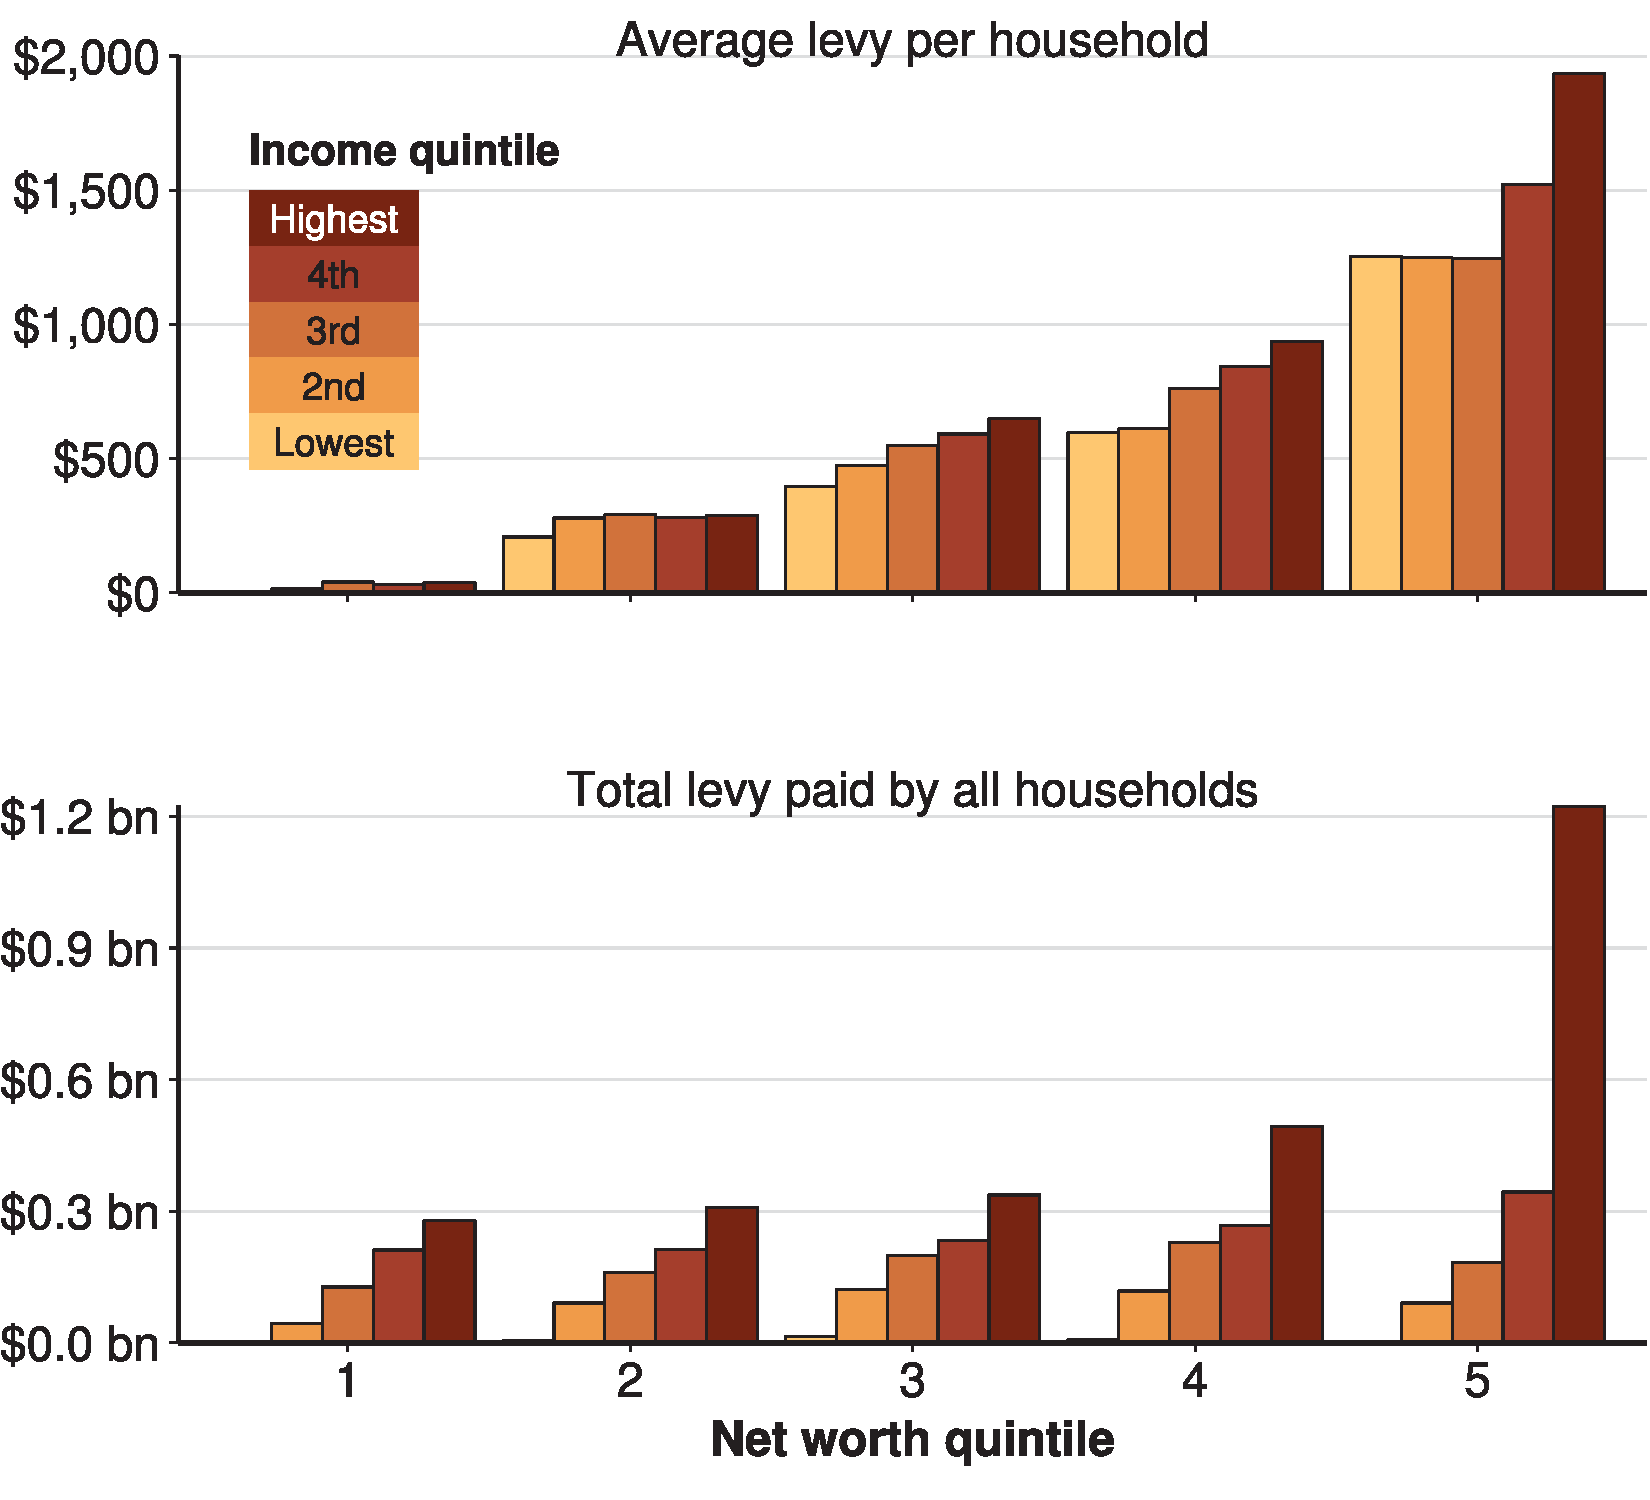
\includegraphics[width=\columnwidth]{Property-taxes/atlas/figure/Figure11-1.pdf}
\notes{2011-12 dollars; Simulated impact of applying a 0.2~per~cent levy to land values only; Households that have reported negative household disposable income and negative net wealth have been excluded from the analysis; quintiles are grouped by equivalised disposable (\ie~post tax) income and net worth of each household.}

\source{\textcite{ABS2013t}; Grattan analysis.}
\end{figure}

\begin{figure}
\caption{The burden would be lowest for low wealth households\label{fig:PROP-12}}%
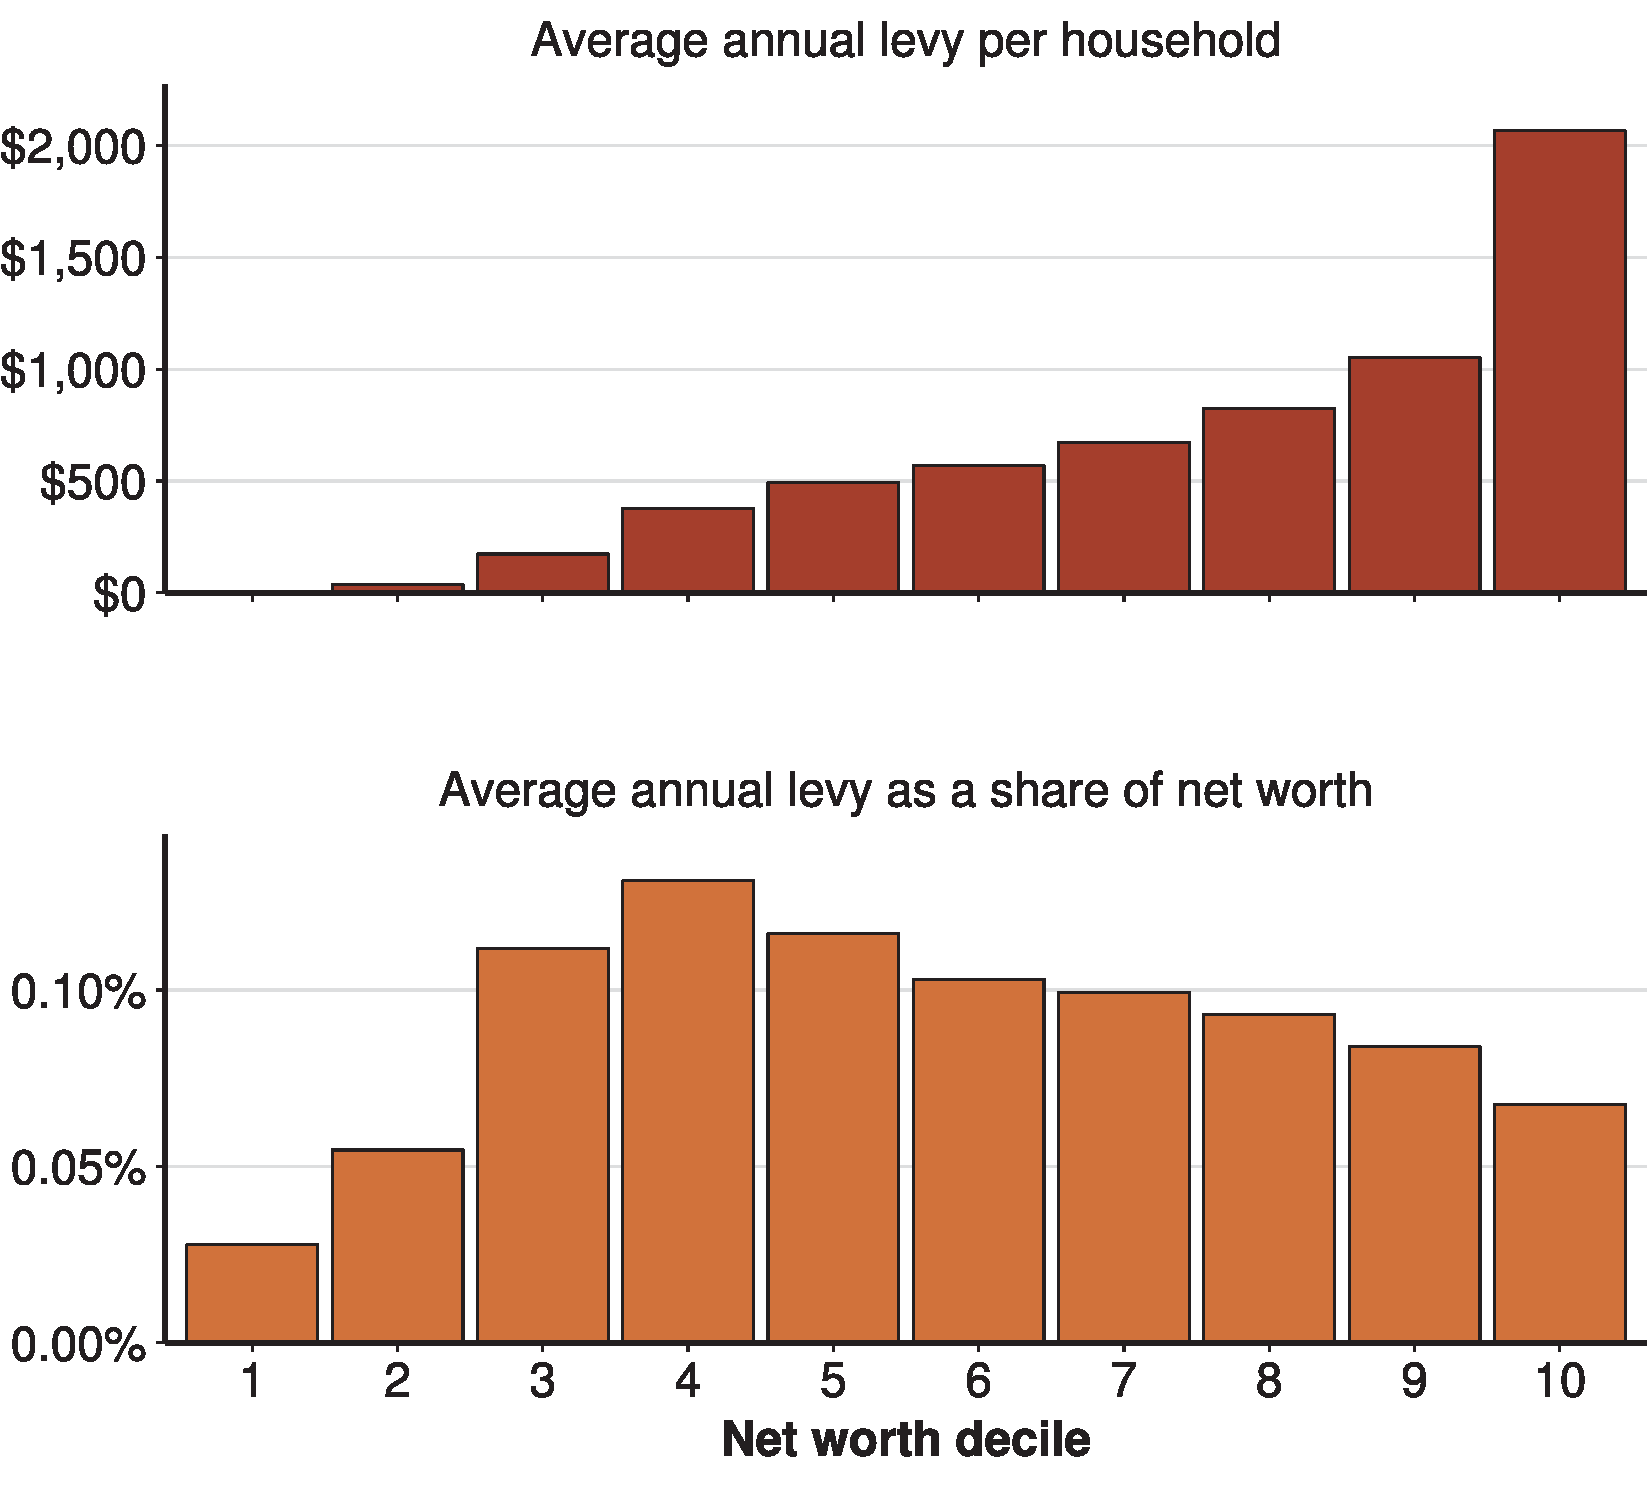
\includegraphics[width=\columnwidth]{Property-taxes/atlas/figure/Figure12-1.pdf}
%{\color{white}%
%\captionsetup{font={\color{white}}}
%\notes{2011-12 dollars; Simulated impact of applying a 0.2~per~cent levy to land values only; Households that have reported negative household disposable income and negative net wealth have been excluded from the analysis; quintiles are grouped by equivalised disposable (\ie~post tax) income and net worth of each household.}

%\source{\textcite{ABS2013t}; Grattan analysis.}%
%}
\end{figure}

\begin{subappendices}
\chapter{State tax revenue growth and revenue volatility\label{appendix:PROP}}
\Cref{sec:PROP-3-2} analyses trends in growth in revenues from major state taxes, and the volatility of those revenues for the period 1990-91 to 2013-14, for all states combined. The aggregate trends over this 25 year period were:

\begin{itemize}
\item	State property taxes such as land tax and stamp duty grew faster than other state taxes;
\item	State property taxes revenues were more volatile than other state taxes;
\item	Our proposed broad-based property levy would have been less volatile than other property taxes, especially stamp duty.
\end{itemize}

However, trends in state tax revenues varied across states, and across different time periods. State-specific economic developments affected the growth in state tax bases, and the volatility of state tax revenue streams. Meanwhile explicit tax policy changes by state governments also affected revenues.

This appendix breaks down in more detail the trends in revenue growth and revenue volatility among major state taxes for the five largest states: New South Wales, Victoria, Queensland, Western Australia and South Australia. Trends in revenue growth and revenue volatility for each of these states are presented over three time periods: 1990-91 to 2013-14, 1990-91 to 1999-2000, and 2000-01 to 2013-14. Trends in revenue growth and volatility for all states combined are also presented for two sub-periods: 1990-91 to 1999-2000; and 2000-2001 to 2013-14.

The trends in revenue growth and revenue volatility in individual states are generally consistent with the national averages. Compared to other property taxes, a broad based property levy would have produced faster growing, more stable revenues for most states, across most time periods.

However, there are some exceptions.  

Over the period 2000-01 to 2013-14, stamp duty revenues grew slower than Gross State Product (GSP) in New South Wales, Queensland and Western Australia (\Vref{fig:PROP-17}). Weaker than average property markets in this period caused a significant fall in stamp duty revenue for these states over these periods, particularly during the Global Financial Crisis. 

In New South Wales, the property market was particularly weak between 2002-03 and  2008-09, with a fall in the number of property transfers leading to lower revenues from stamp duties on conveyances.\footcite[][18]{CGC2009a}  The median price of houses transacted in Sydney grew by only 21.4~per~cent over this period, while the total number of property transfers fell by more than 30~per~cent.\footcite{ABS2015ResidentialPropertyIndex}  

In Queensland, the state government lifted the exemption threshold on stamp duty for first-home buyers from \$320,000 to \$500,000 in 2008-09, eroding the tax base.\footcite{TreasuryTradeQld2012}  The Queensland property market also declined after the GFC. The median price of houses transacted in Brisbane fell by an average of 5~per~cent between 2008 and 2012, whereas GSP increased by 23~per~cent over the same period.  

Queensland revenues from a broad-based property levy would have grown slower than GSP over the period 1990 to 1999. In this period, total land value increased by only 60~per~cent, compared to the approximately 300~per cent increase in total land value over the period 2000 to 2013.\footnote{\gao\ \textcite{ABS2014e}.}

In Western Australia, stamp duties fell from 15.4~per~cent of state revenues in 2005-06 to 10.6~per~cent in 2008-09, due to a similar decline in the property market.\footcite[][13]{CGC2010b}   The median price of houses transacted in Perth fell by 10~per~cent between 2008 and 2012, whereas GSP rose by 56~per~cent over the same period. Moreover, the Western Australian State Government doubled the exemption threshold on stamp duties for first-home buyers in 2007-08, lifting the threshold for residential properties to \$500,000.  In 2008-09, stamp duties for residential properties were also lowered, with a 15~per~cent cut to stamp duty on a median price house. \footcite{Treasury2007a}   This further eroded the tax base, where residential land value accounted for over 75~per~cent of total land value in Western Australia.\footcite{Treasury2008a}

\cleardoubleevenstandardpage
\newcommand{\propPhantomNotes}{
{\color{white}
\notes{‘Property levy’ shows the revenues that would have been raised with a broad-based property levy of 0.2~per~cent applied to unimproved land values had it been in place over the period.}

\source{\textcites{ABSmultipleyears}{ABS2014e}; Grattan analysis.}}
}

\begin{figure}
\captionwithunits{Revenue from property taxes grew slower than many other taxes between 1990 and 2000}%
{Percentage change in tax revenue for a 10~per~cent increase in Gross State Product, 1990-91 to 1999-2000}%
\includegraphics[width=\columnwidth,page=18]{Property-taxes/atlas/PPTXProperty.pdf}
\notes{‘Property levy’ shows the revenues that would have been raised with a broad-based property levy of 0.2~per~cent applied to unimproved land values had it been in place over the period.}

\source{\textcites{ABSmultipleyears}{ABS2014e}; Grattan analysis.}
\end{figure}

\begin{figure}
\captionwithunits{Revenue from property taxes grew faster than many other taxes since 2000}%
{Percentage change in tax revenue for a 10~per~cent increase in Gross State Product, 2000-01 to 2013-14}%
\includegraphics[width=\columnwidth,page=19]{Property-taxes/atlas/PPTXProperty.pdf}
\propPhantomNotes
\end{figure}

\begin{figure}
\captionwithunits{\label{fig:PROP-17}A broad-based property levy would have been less volatile than other property taxes, and many other taxes between 1990 and 2000}%
{Standard deviation between annual revenue growth and long run average growth, 1990-91 to 1999-2000}
\includegraphics[width=\columnwidth,page=20]{Property-taxes/atlas/PPTXProperty.pdf}
\propPhantomNotes
\end{figure}

\begin{figure}
\captionwithunits{A broad-based property levy would have been less volatile than other property taxes, except in WA, since 2000}%
{Standard deviation between annual revenue growth and long run average growth, 1990-91 to 1999-2000}
\includegraphics[width=\columnwidth,page=21]{Property-taxes/atlas/PPTXProperty.pdf}
\propPhantomNotes
\end{figure}

\begin{figure}
\captionwithunits{Unlike most other taxes, a broad-based property levy would have grown faster than GDP between 1990 and 2000, and between 2000 and 2014}%
{Percentage change in tax revenue for a 10~per~cent increase in national GDP, all states}
\includegraphics[width=\columnwidth,page=22]{Property-taxes/atlas/PPTXProperty.pdf}
\propPhantomNotes
\end{figure}

\begin{figure}
\captionwithunits{A broad-based property levy would have been less volatile than other property taxes between 1990 and 2000, and between 2000 and 2014}%
{Standard deviation between annual revenue growth and long run average growth, all states}
\includegraphics[width=\columnwidth,page=23]{Property-taxes/atlas/PPTXProperty.pdf}
\propPhantomNotes
\end{figure}


\end{subappendices}

\part{Super tax targeting}\label{part:SUPER}
\subimport*{Super-tax-targeting/}{b5-Diana-portrait-Super-tax-targeting-as-chapter}

\part{A GST reform package}\label{part:GST}
\subimport*{GST-reform-package/}{b5-Diana-portrait-GST-reform-package-as-chapter}

\part{Negative gearing and the capital gains tax discount}
\subimport*{Hot-property-CG-and-NG/}{b5-Dianna-CGT_and_neg_gearing_final-as-chapter.tex}




\nocite{R-ggrepel,R-testthat,R-taxstats,R-magrittr,R-tidyr,R-devtools,R-expm,R-Matrix,R-Hmisc,R-Formula,R-survival,R-lattice,R-foreign,R-survey,R-zoo,R-httr,R-rsdmx,R-readr,R-openxlsx,R-readxl,R-xtable,R-grattan,R-directlabels,R-scales,R-ggplot2,R-gridExtra,R-dplyr,R-data.table,R-devEMF,R-knitr}

\backmatter
\addpart*{Endnotes and references}\addcontentsline{toc}{part}{Endnotes and references}
\addchap{Lists of tables and figures}
\clearpage
\small
\listoffigures
\printfigurenotes
\cleardoublepage
\listoftables
\printtablenotes
\cleardoublepage

\printendnotes[custom]
\addchap{Bibliography}
\printbibliography[title={Bibliography},heading=none]
\end{document}
